\chapter{Temporality Adaptation}
\label{chp:temporality}

\section{Introduction}
Language changes and varies over time,
which can cause a degradation of performance in
natural language processing (NLP) models over time.
For example, document classifiers are typically trained on historical data and tested on future data, where the performance tends to be worse.
Recent research has shown that document classifiers can become more stable over time when trained in ways that specifically account for temporal variations~\cite{he2018time}.
We refer to this task of accounting for such variations during training as {\em temporality adaptation}.
This chapter is based on materials from~\cite{huang2018examining, huang2019neural}.\footnote{The datasets along with the code are available on: \\\url{https://github.com/xiaoleihuang/Neural_Temporality_Adaptation}, \\\url{https://github.com/xiaoleihuang/Domain_Adaptation_ACL2018}.}

This chapter has three main parts.
It starts with introducing six English and Chinese datasets from both social media and newspaper sources, spanning varying lengths in time (from several decades to only a few years) in Section~\ref{chap3:sec:data}. 
Each dataset is split into a small set of time intervals, and we define each time interval as a domain. 
The section analyzes language shifts from three aspects: word, topic and context. 
Moreover, the section investigates how language shifts impact the performance of document classifiers.
The Section~\ref{chap3:sec:fa} and \ref{chap3:sec:dwe} propose two temporality adaptation methods via feature augmentation and diachronic word embedding (DWE).

The first method uses \textit{feature augmentation} to integrate the temporal factor into document classifiers.
The approach considers both long-term variations in text over the years and seasonal variations that change throughout a year but repeat across years.
The proposed method extends the existing domain adaptation method~\cite{daume2007frustratingly} and augments document representations by using both time domain-dependent and domain-independent features to train classifiers.
While the training process uses both domain-dependent and -independent features, the testing phase only uses domain-independent feature sets.
The goal is to learn and train domain-independent document features and classifiers.
The experiments show that out-of-the-box domain adaptation techniques can make $n$-gram classifiers more robust to temporal shifts.

The second approach explores temporality adaptation from the {\em diachronic} word embeddings~\cite{kutuzov2018diachronic} perspective and further integrates the dynamic word embeddings into a time-driven neural classifier.
The proposed diachronic word embedding learns dynamic word representations from the subword level, where the embedding model represents a word by its subword components. 
Evaluation on a standard news corpus proves the effectiveness of our proposed DWE model. 
To adapt temporality into document classifiers, we propose a time-driven neural classifier that encodes documents in the view of diachronic word embeddings.
Experiments on several time-varying classification datasets demonstrate that diachronic word embedding can generally improve model performance and the proposed time-driven classifier consistently outperforms strong baselines. 

% Main contributions
Detailed contributions of this chapter as follows:

\begin{enumerate}
    \item We conducted a detailed analysis to understand the relation between language shifts and important features for document classification. We examine language shifts from the word, context, topic and semantic aspects.
    \item We applied a simple domain adaptation method via feature augmentation on both yearly and monthly varying corpora.
    \item We proposed a subword-level method for constructing diachronic words embeddings, which we show to be competitive with prior approaches. 
    \item Our results show that neural classifiers that use diachronic word embeddings can perform better on future data. 
\end{enumerate}


\section{Related Work}
\label{chap3:sec:survey}

Language evolves with the increasing available online data over time. 
With recent progress in deep neural representation learning, emerging work has been probing into the language shifting issue from the view of diachronic or dynamic word embedding perspective~\cite{tang2018state, kutuzov2018diachronic}.
These studies have shown that shifts in the language across time cause changes in word contexts and consequently, changes in the learned representations. 

Existing research~\cite{kim2014temporal, hamilton2016diachronic, yao2018dynamic, kutuzov2018diachronic} learns diachronic word embeddings from the word level, which creates a word representation in each period separately for the same word.
To encode the temporal factor into embedding models, existing methods develop three main directions, incremental training~\cite{kim2014temporal}, linear alignment~\cite{kulkarni2015statistically, hamilton2016diachronic} and vector representation~\cite{rosenfeld2018deep, huang2019neural}.
We illustrate the process of building a regular DWE in Section~\ref{chap2:sec:dwe}.
However, such a method has three issues: first, building a separate embedding model for each time interval has a high time-complexity cost, memory and space; second, the colloquium and misspelling words in social media data degrade the effectiveness of word-level embeddings; third, the fixed size of the model vocabulary across periods may not be robust enough for future incoming new words.
In this chapter, we treat the time as a subword component and vectorize the component into a fixed length of numerical representation.


Time is implicitly embedded in the document classification process: 
classifiers are often built to be applied to future data that doesn't yet exist,
and performance on held-out data is measured to estimate performance on future data whose distribution may have changed.
Methods exist to adjust for changes in the data distribution ({\em covariate shift}) \cite{shimodaira2000improving, bickel2009discriminative},
but time is not typically incorporated into such methods explicitly.
One line of work that explicitly studies the relationship between time and the distribution of data is work on classifying time in which a document was written ({\em document dating}) \cite{kanhabua2008improving, chambers2012labeling, kotsakos2014burstines}.
However, this task is directed differently from our work: predicting timestamps given documents, rather than predicting information about documents given timestamps.
Recent work~\cite{desai2019adaptive} used the student and teacher framework to constrained feature variations across domains for classifying whether documents are political, however, the main experimental settings in the work are different from ours, which the training set does not have periods and do not explicitly augment document representations on the time. 
The work mainly focused on different source domains (New York Times vs. others) instead of the temporal domain which is our main focus in this thesis.
While research has applied diachronic word embeddings to semantic change detection and validation~\cite{mihalcea2012word, kim2014temporal, kulkarni2015statistically, hamilton2016diachronic, dubossarsky2017outta, yao2018dynamic, rudolph2018dynamic, rosenfeld2018deep, hu2019diachronic}, semantic relation analysis~\cite{liao2016analysing, szymanski2017temporal, rosin2017learning} and recent work in the named entity recognition~\cite{rijhwani2020temporally}, these types of embeddings have not been studied particularly for the document classification task, which is our focus in this chapter.


\section{Time-Varying Corpora}
\label{chap3:sec:data}

The way people use words to express opinions has been constantly changing over time~\cite{mihalcea2012word, kulkarni2015statistically, hamilton2016diachronic}. In this section, we introduce our corpora in English and Chinese including both news articles and social media data. We conduct exploratory analyses on how language shifts over time with respect to the task of classification. The exploration of language shifts investigates several perspectives: word usage variation, context shift and topic change. We then examine how language variations impact the document classification task.

\subsection{Data}
We retrieved available data sources from previous publications~\cite{zhang2014explicit, he2016ups, huang2018examining}. Specifically, we use four different sources in English---Amazon (music reviews), Yelp (restaurant and hotel reviews), Twitter (vaccine tweets), economic newspaper articles~\cite{figure_eight_2015} and political sentences\footnote{The American party platforms of Republicans and Democrats from 1948 to 2016, available every four years. Retrieved from \url{https://www.comparativeagendas.net/datasets_codebooks}.} and one source in Chinese, Dianping~\cite{meituan-dianping_2019}.
\textit{Dianping} is a Chinese platform for reviewing locally found consumer products and retail services, akin to Yelp.
The \textit{Twitter} data is annotated with binary labels indicating whether a user received an influenza vaccination (i.e., a flu shot)~\cite{huang2017examining}.
The \textit{Economy} data is annotated with binary labels indicating if each article relates to the US economy. 
For the review data (\textit{Amazon, Dianping} and \textit{Yelp}), we encode the review scores according to the experimental settings in Section~\ref{chap3:sec:fa} and Section~\ref{chap3:sec:dwe}. 
We discarded reviews that had fewer than 10 tokens or a helpfulness/usefulness score of zero. 

Our experiments require documents to be grouped into time intervals.
Documents that fall outside of these time intervals were removed. 
We group the corpora into the following two types of temporal intervals:

\begin{itemize}
    \item {\bf Seasonal:} Time intervals within a year (e.g., January through March) that may be repeated across years.
    \item {\bf Non-seasonal:} Non-repeating time intervals spanning one or more years (e.g., 1997-1999).
\end{itemize}

Table~\ref{chap3:tab:data} shows the intervals for each corpus. 
We encode each temporal domain into the discrete time labels, $1, 2, ..., T$. Each corpus then can be represented as $C = [C_1, C_2, ..., C_T]$, where each $C_t$ for $t\in T$ is one temporal slice of the document collection.

\begin{table*}
\centering
\resizebox{\textwidth}{!}{
\begin{tabular}{|l|l|l|l|}
\hline
\bf Dataset & \bf Time intervals (non-seasonal) & \bf Time intervals (seasonal) & \bf Size \\
\hline
Amazon & 1997-99, 2000-02, 2003-05, 2006-08, 2009-11, 2012-14 & Jan-Mar, Apr-Jun, Jul-Sep, Oct-Dec & 653K \\
Dianping & 2009, 2010, 2011, 2012 & n/a & 671K  \\
Economy & 1950-70, 1971-85, 1986-2000, 2001-14 & Jan-Mar, Apr-Jun, Jul-Sep, Oct-Dec & 6.29K  \\
Politics & 1948-56, 1960-68, 1972-80, 1984-92, 1996-2004, 2008-16 & n/a & 35.8K  \\
Twitter & 2013, 2014, 2015, 2016 & Jan-Mar, Apr-Jun, Jul-Sep, Oct-Dec & 9.83K  \\
Yelp-hotel & 2005-08, 2009-11, 2012-14, 2015-17 & Jan-Mar, Apr-Jun, Jul-Sep, Oct-Dec & 78.6K \\
Yelp-rest & 2005-08, 2009-11, 2012-14, 2015-17 & Jan-Mar, Apr-Jun, Jul-Sep, Oct-Dec & 1.16M  \\
\hline
\end{tabular}
}
\caption{Descriptions of corpora spanning multiple time intervals. Size is the number of documents. We use Yelp-hotel and -rest to denote the review data for hotel and restaurant categories. The $n/a$ denotes no periods for the corresponding dataset.}
\label{chap3:tab:data}
\end{table*}


\subsection{Analysis 1: Word Usage Shift}
\label{chap3:subsec:wusage}

\begin{figure}[tb!]
\centering
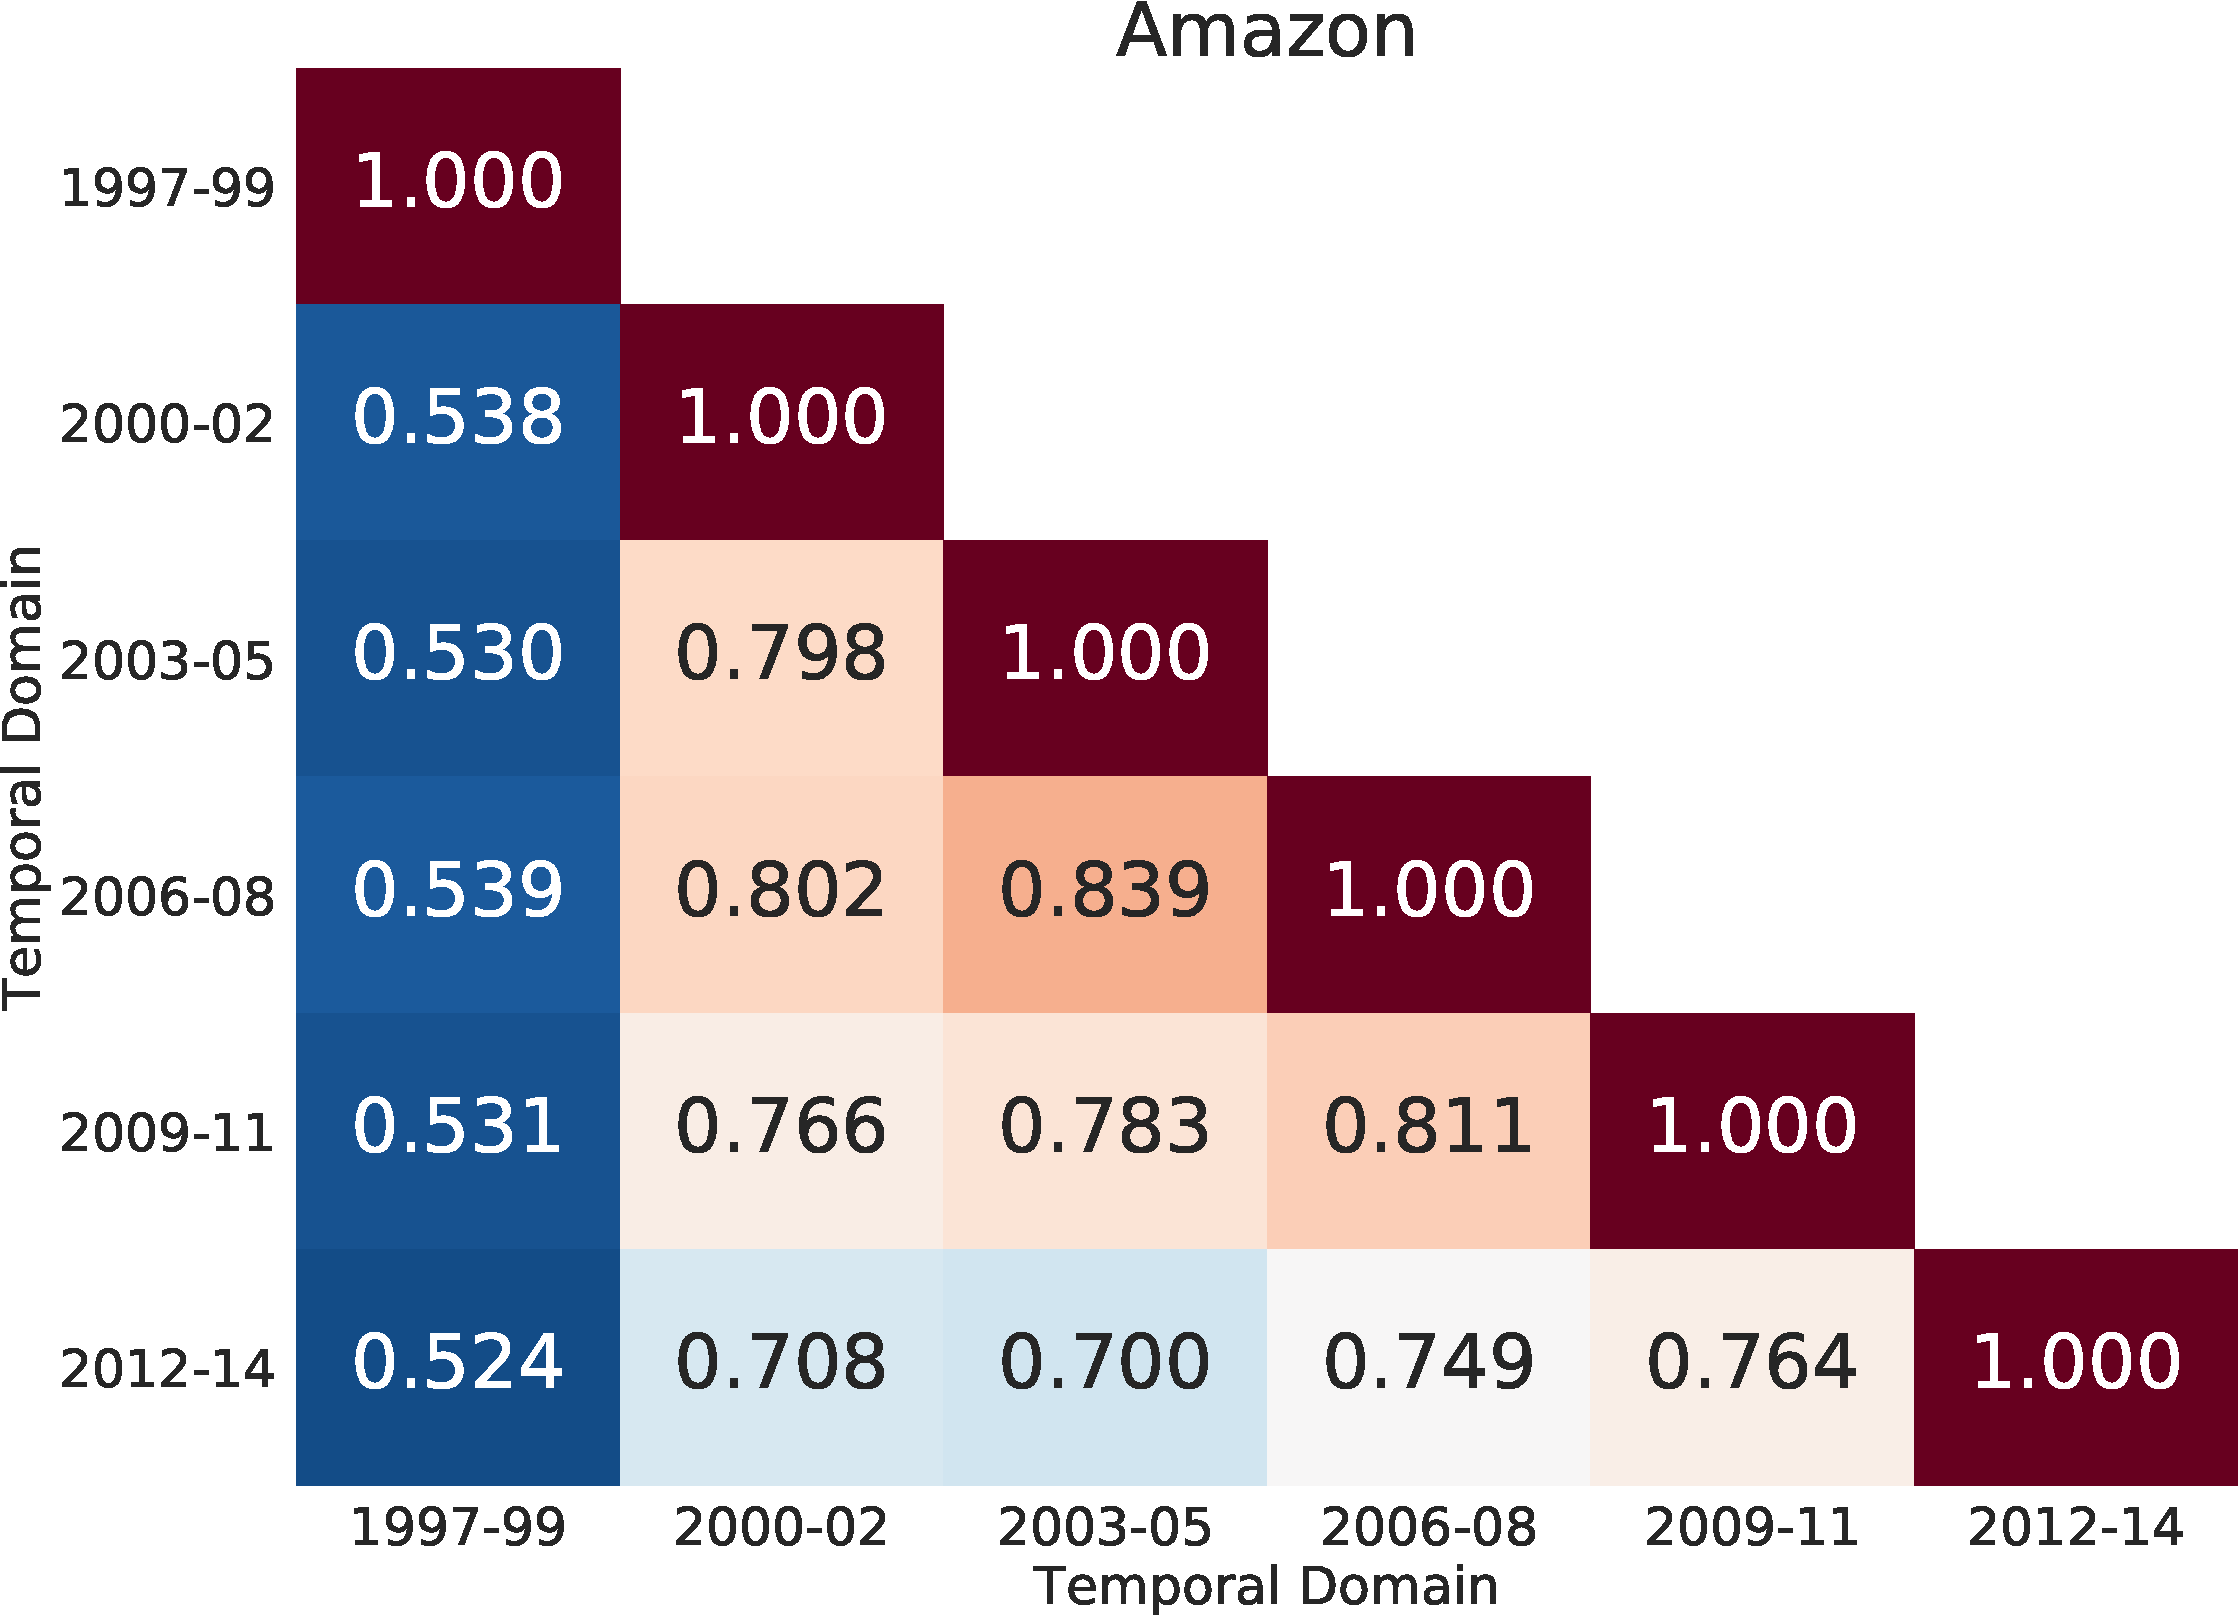
\includegraphics[width=0.32\textwidth]{images/chapter3/lang_use/amazon.pdf}
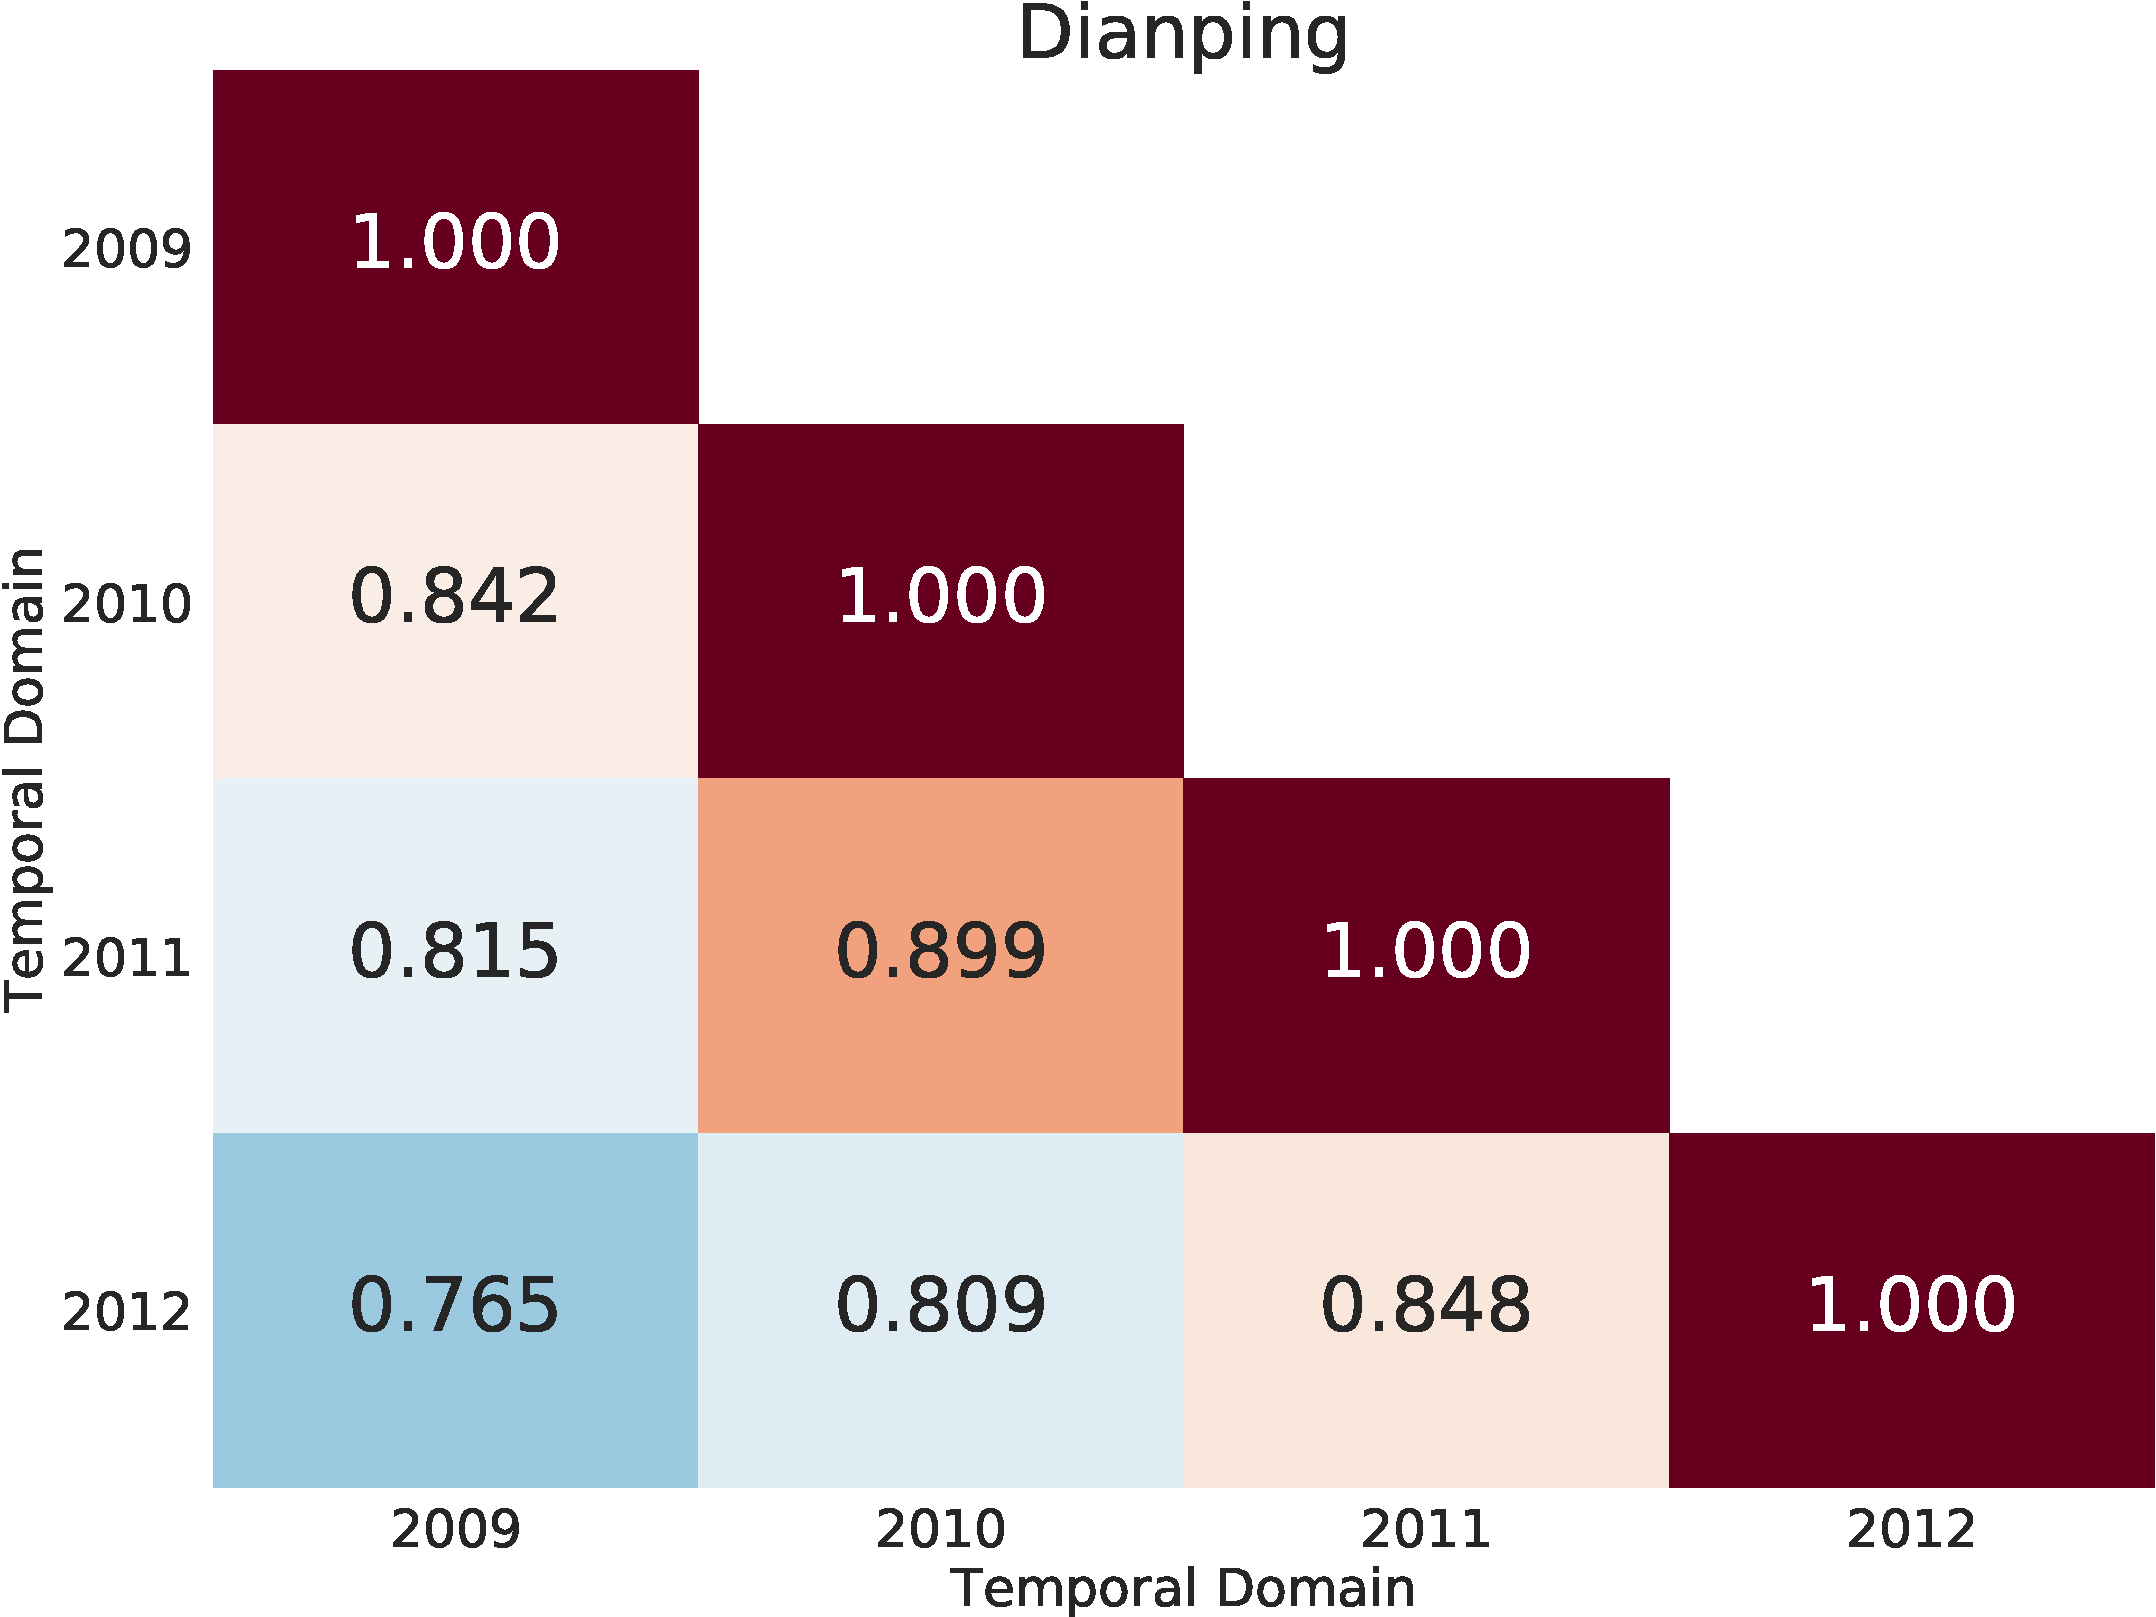
\includegraphics[width=0.32\textwidth]{images/chapter3/lang_use/dianping.pdf}
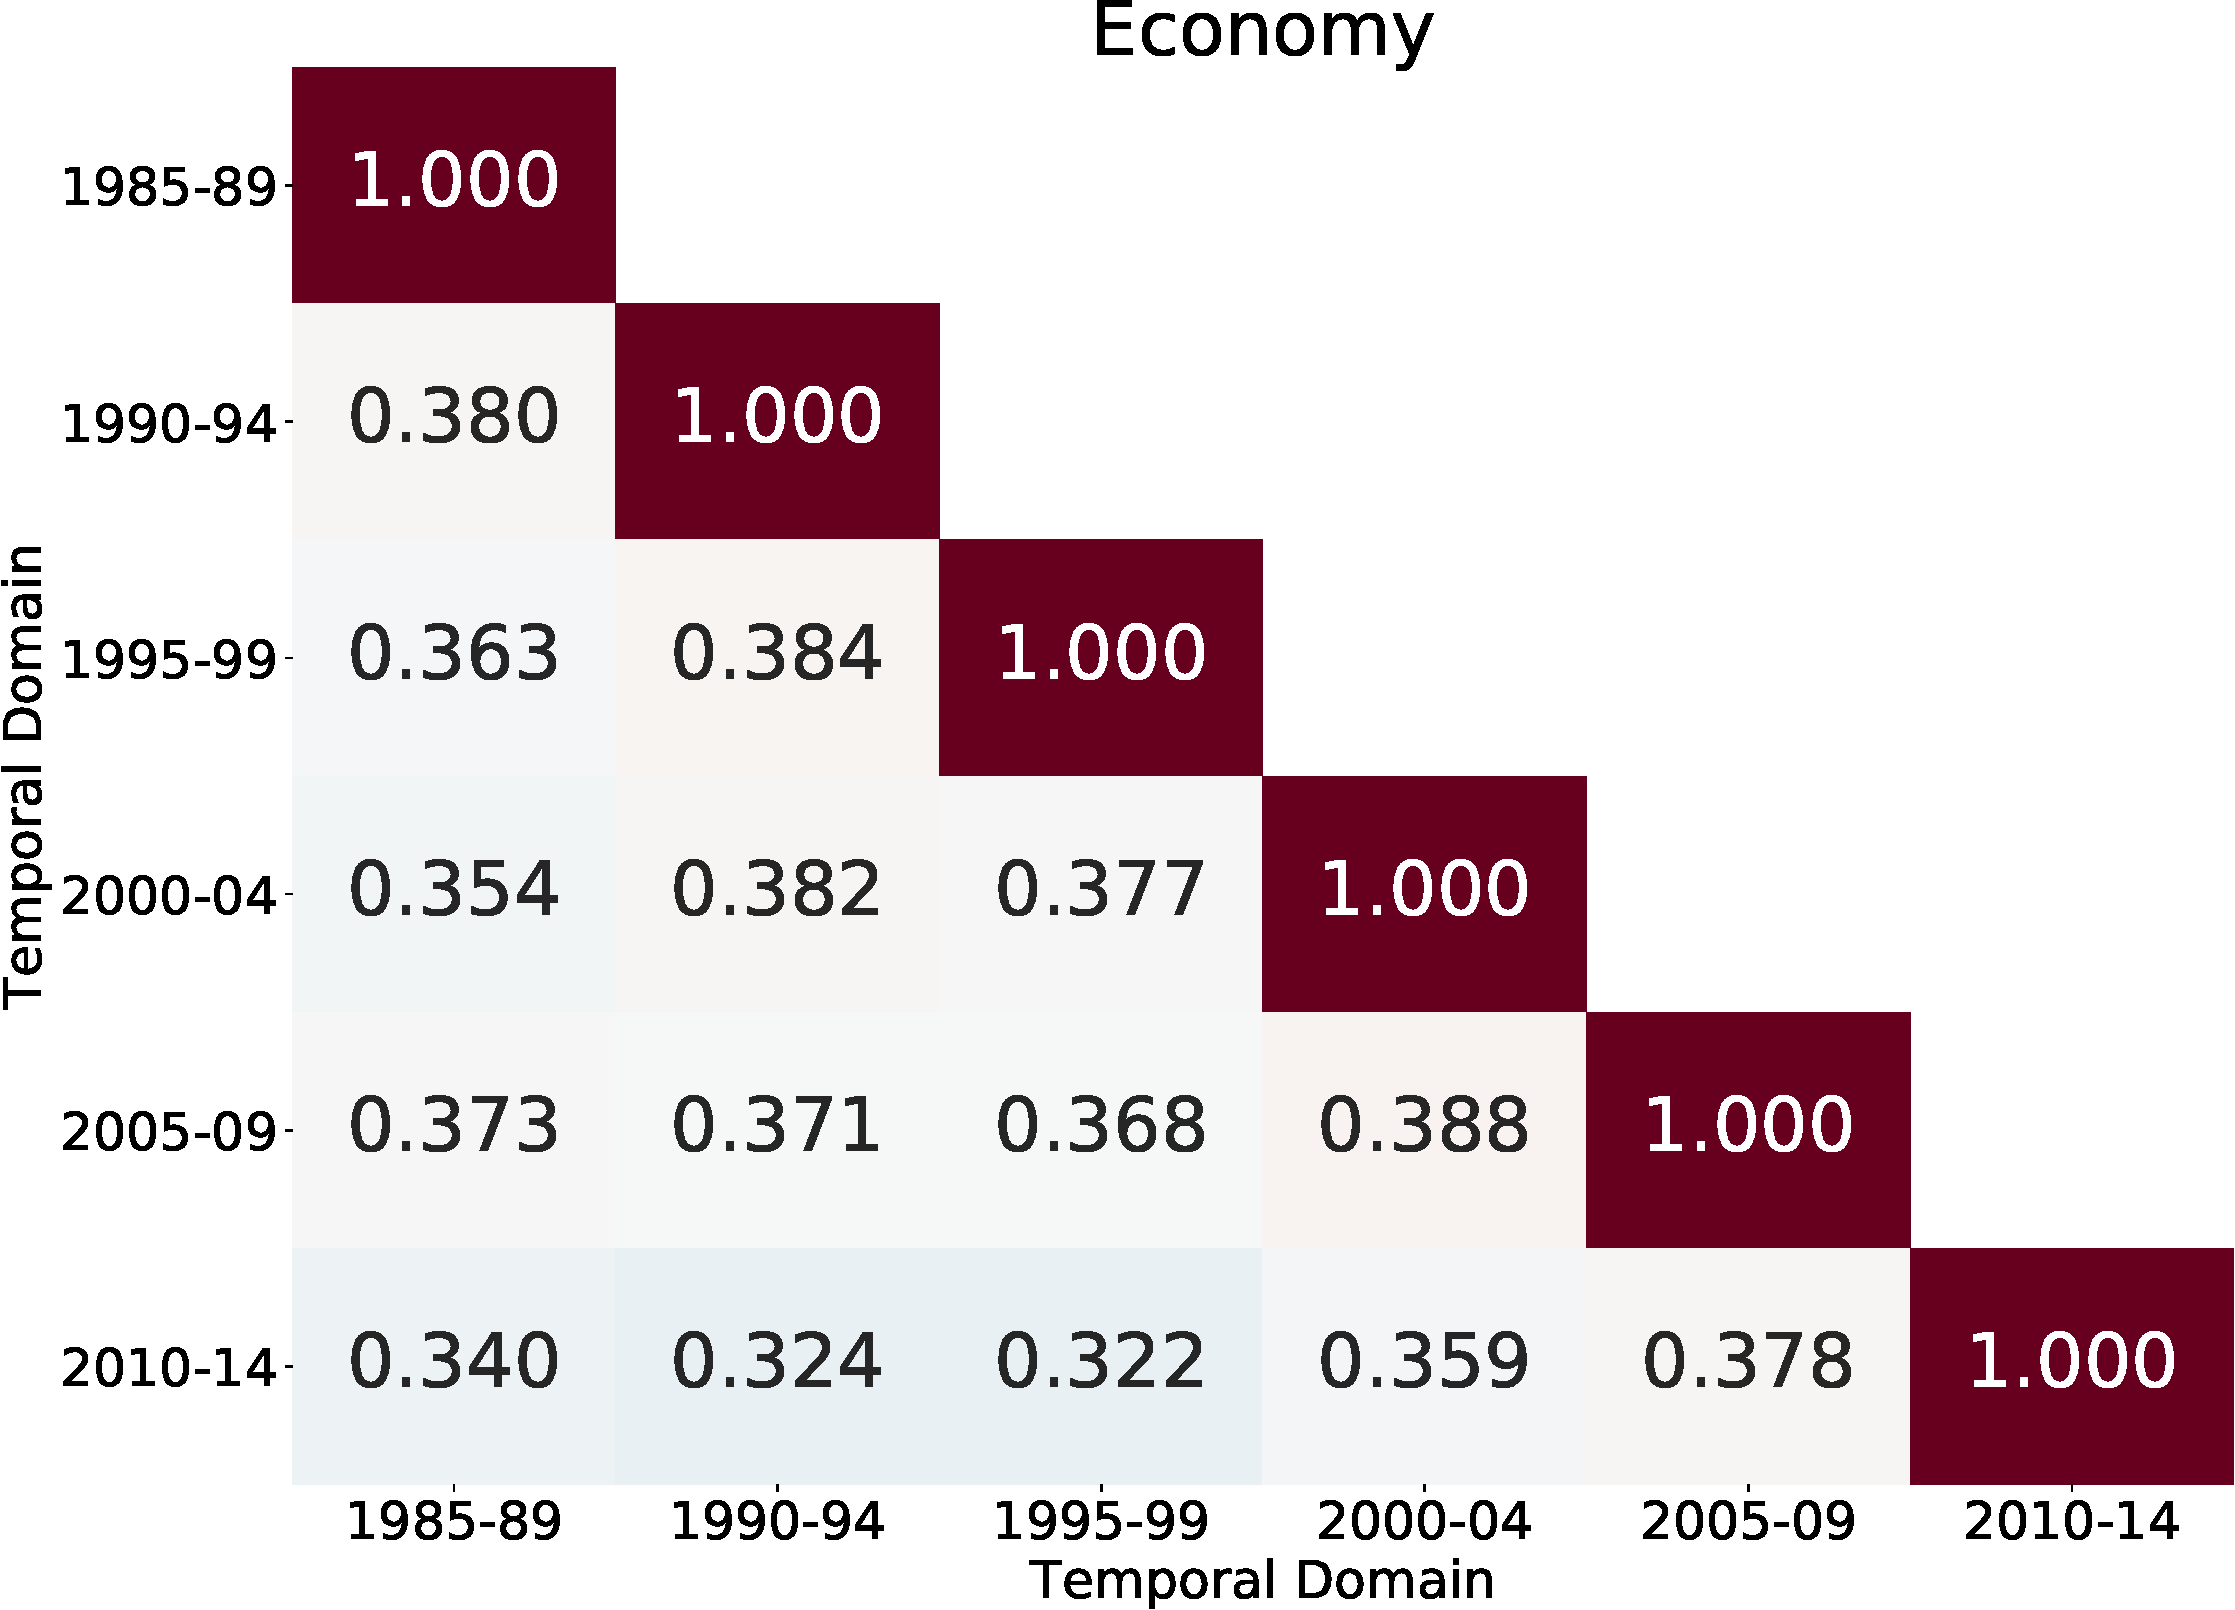
\includegraphics[width=0.32\textwidth]{images/chapter3/lang_use/economy.pdf}
\newline
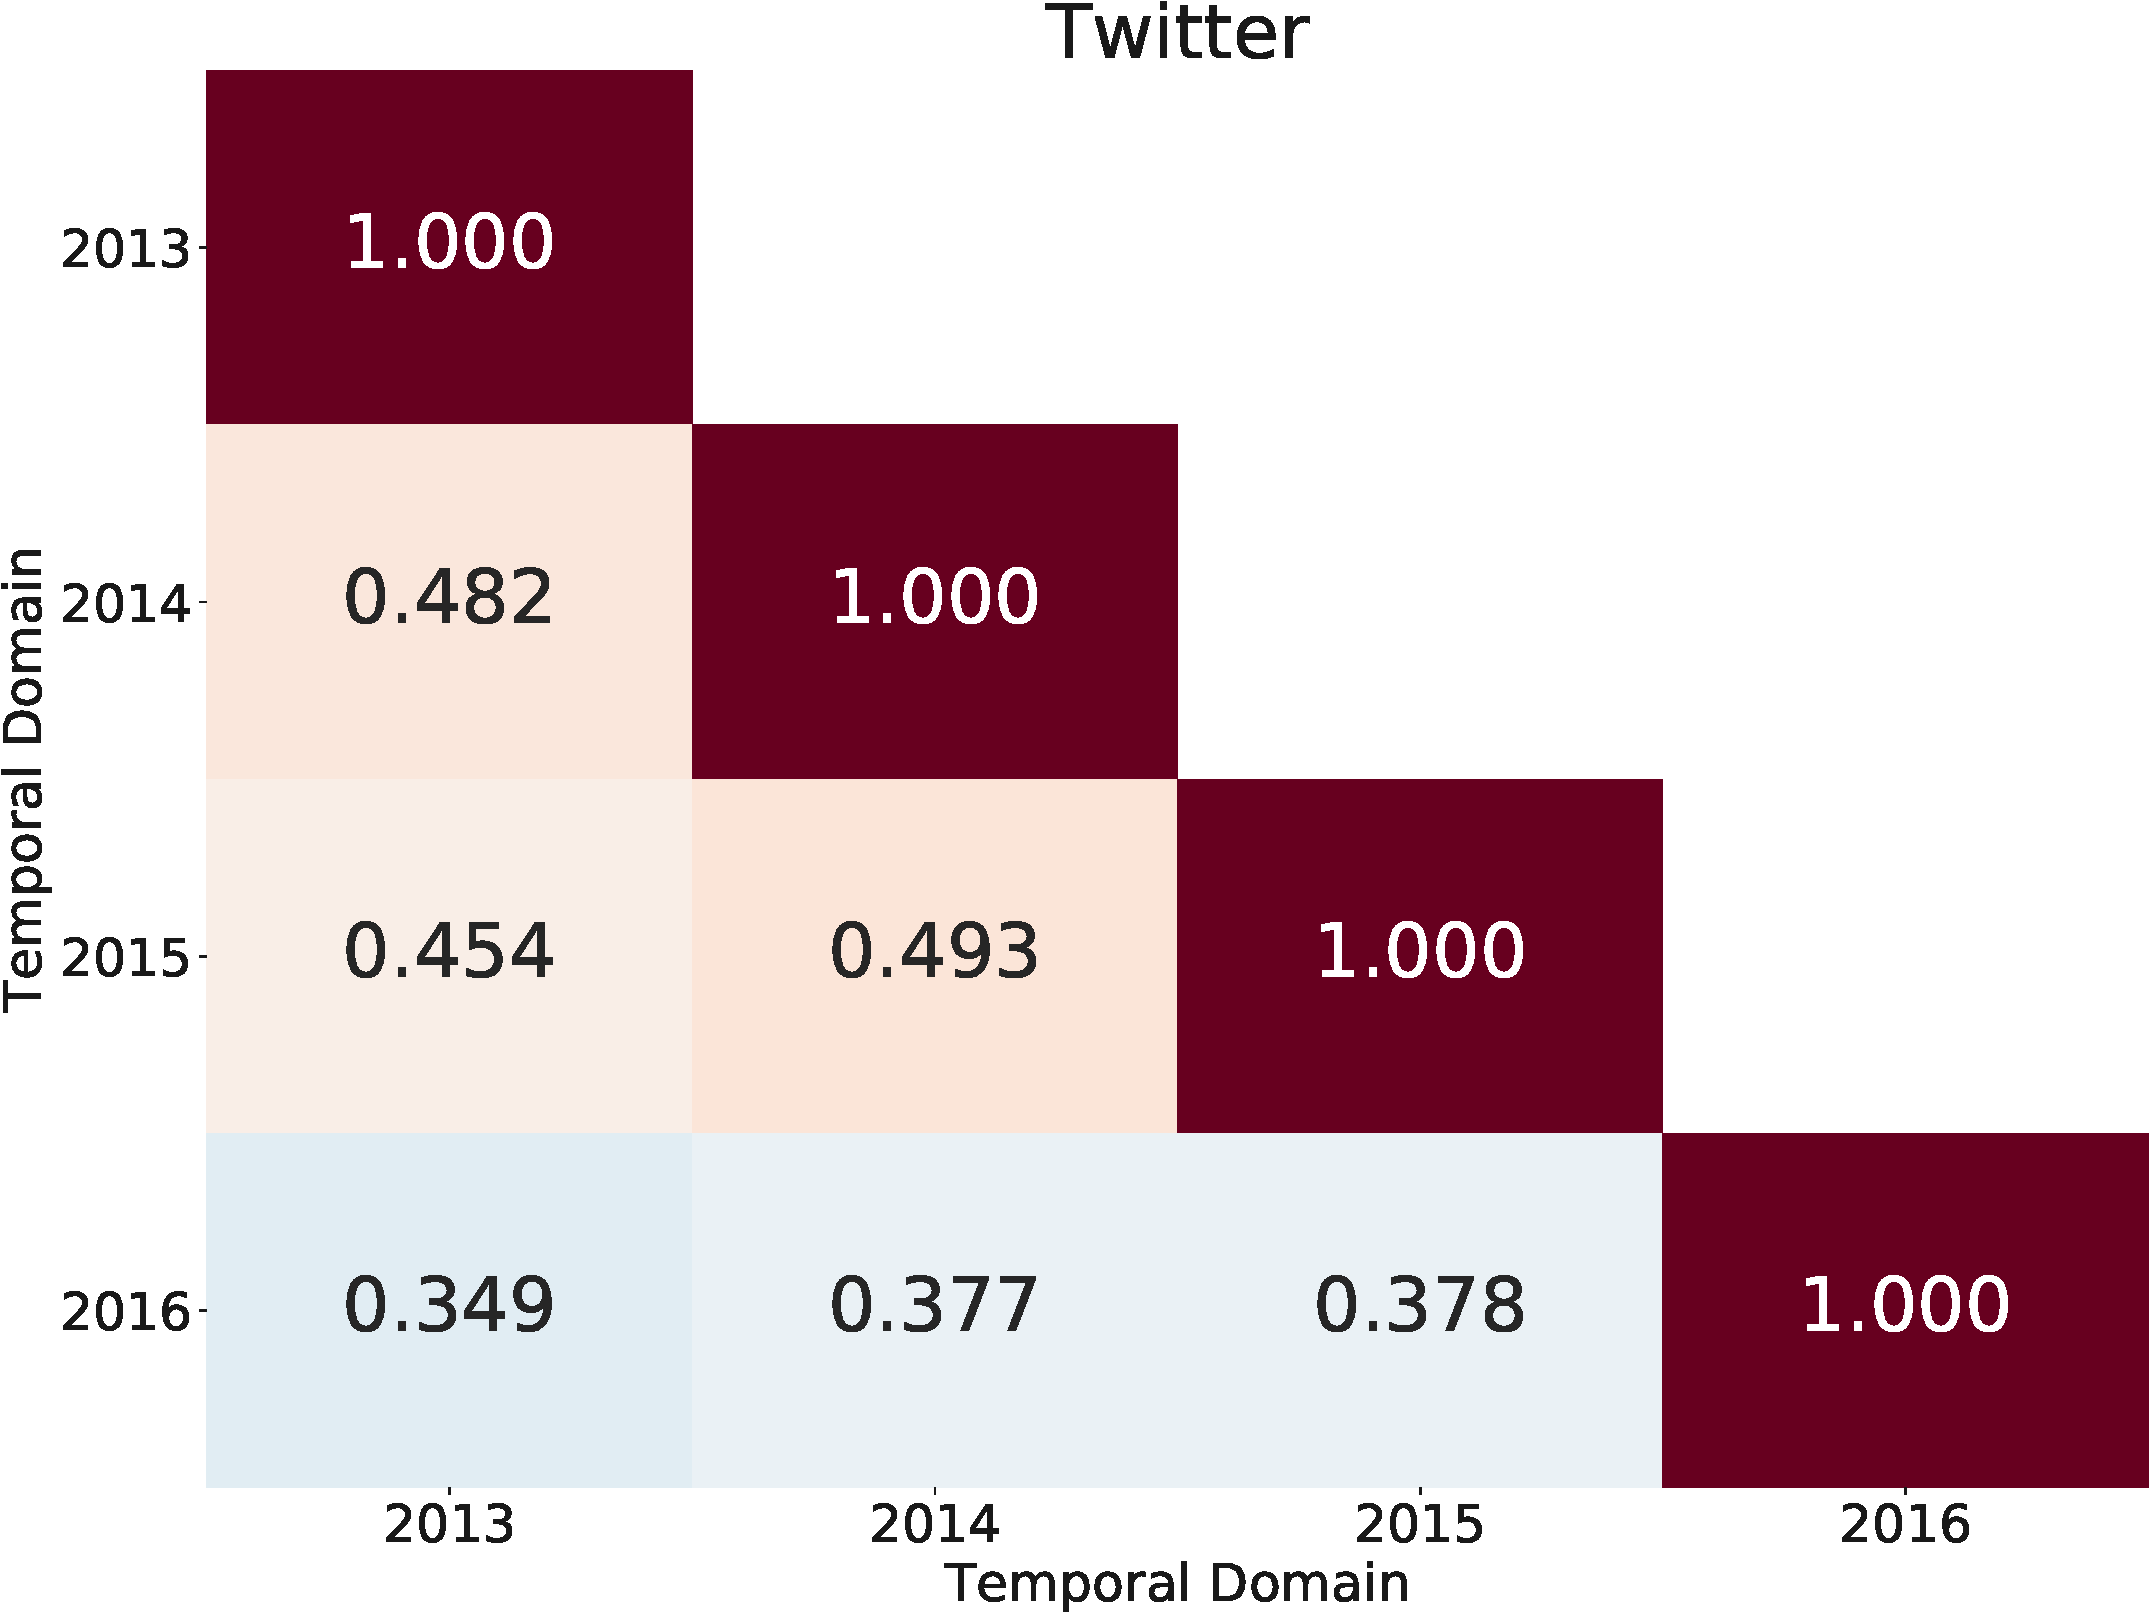
\includegraphics[width=0.32\textwidth]{images/chapter3/lang_use/vaccine.pdf}
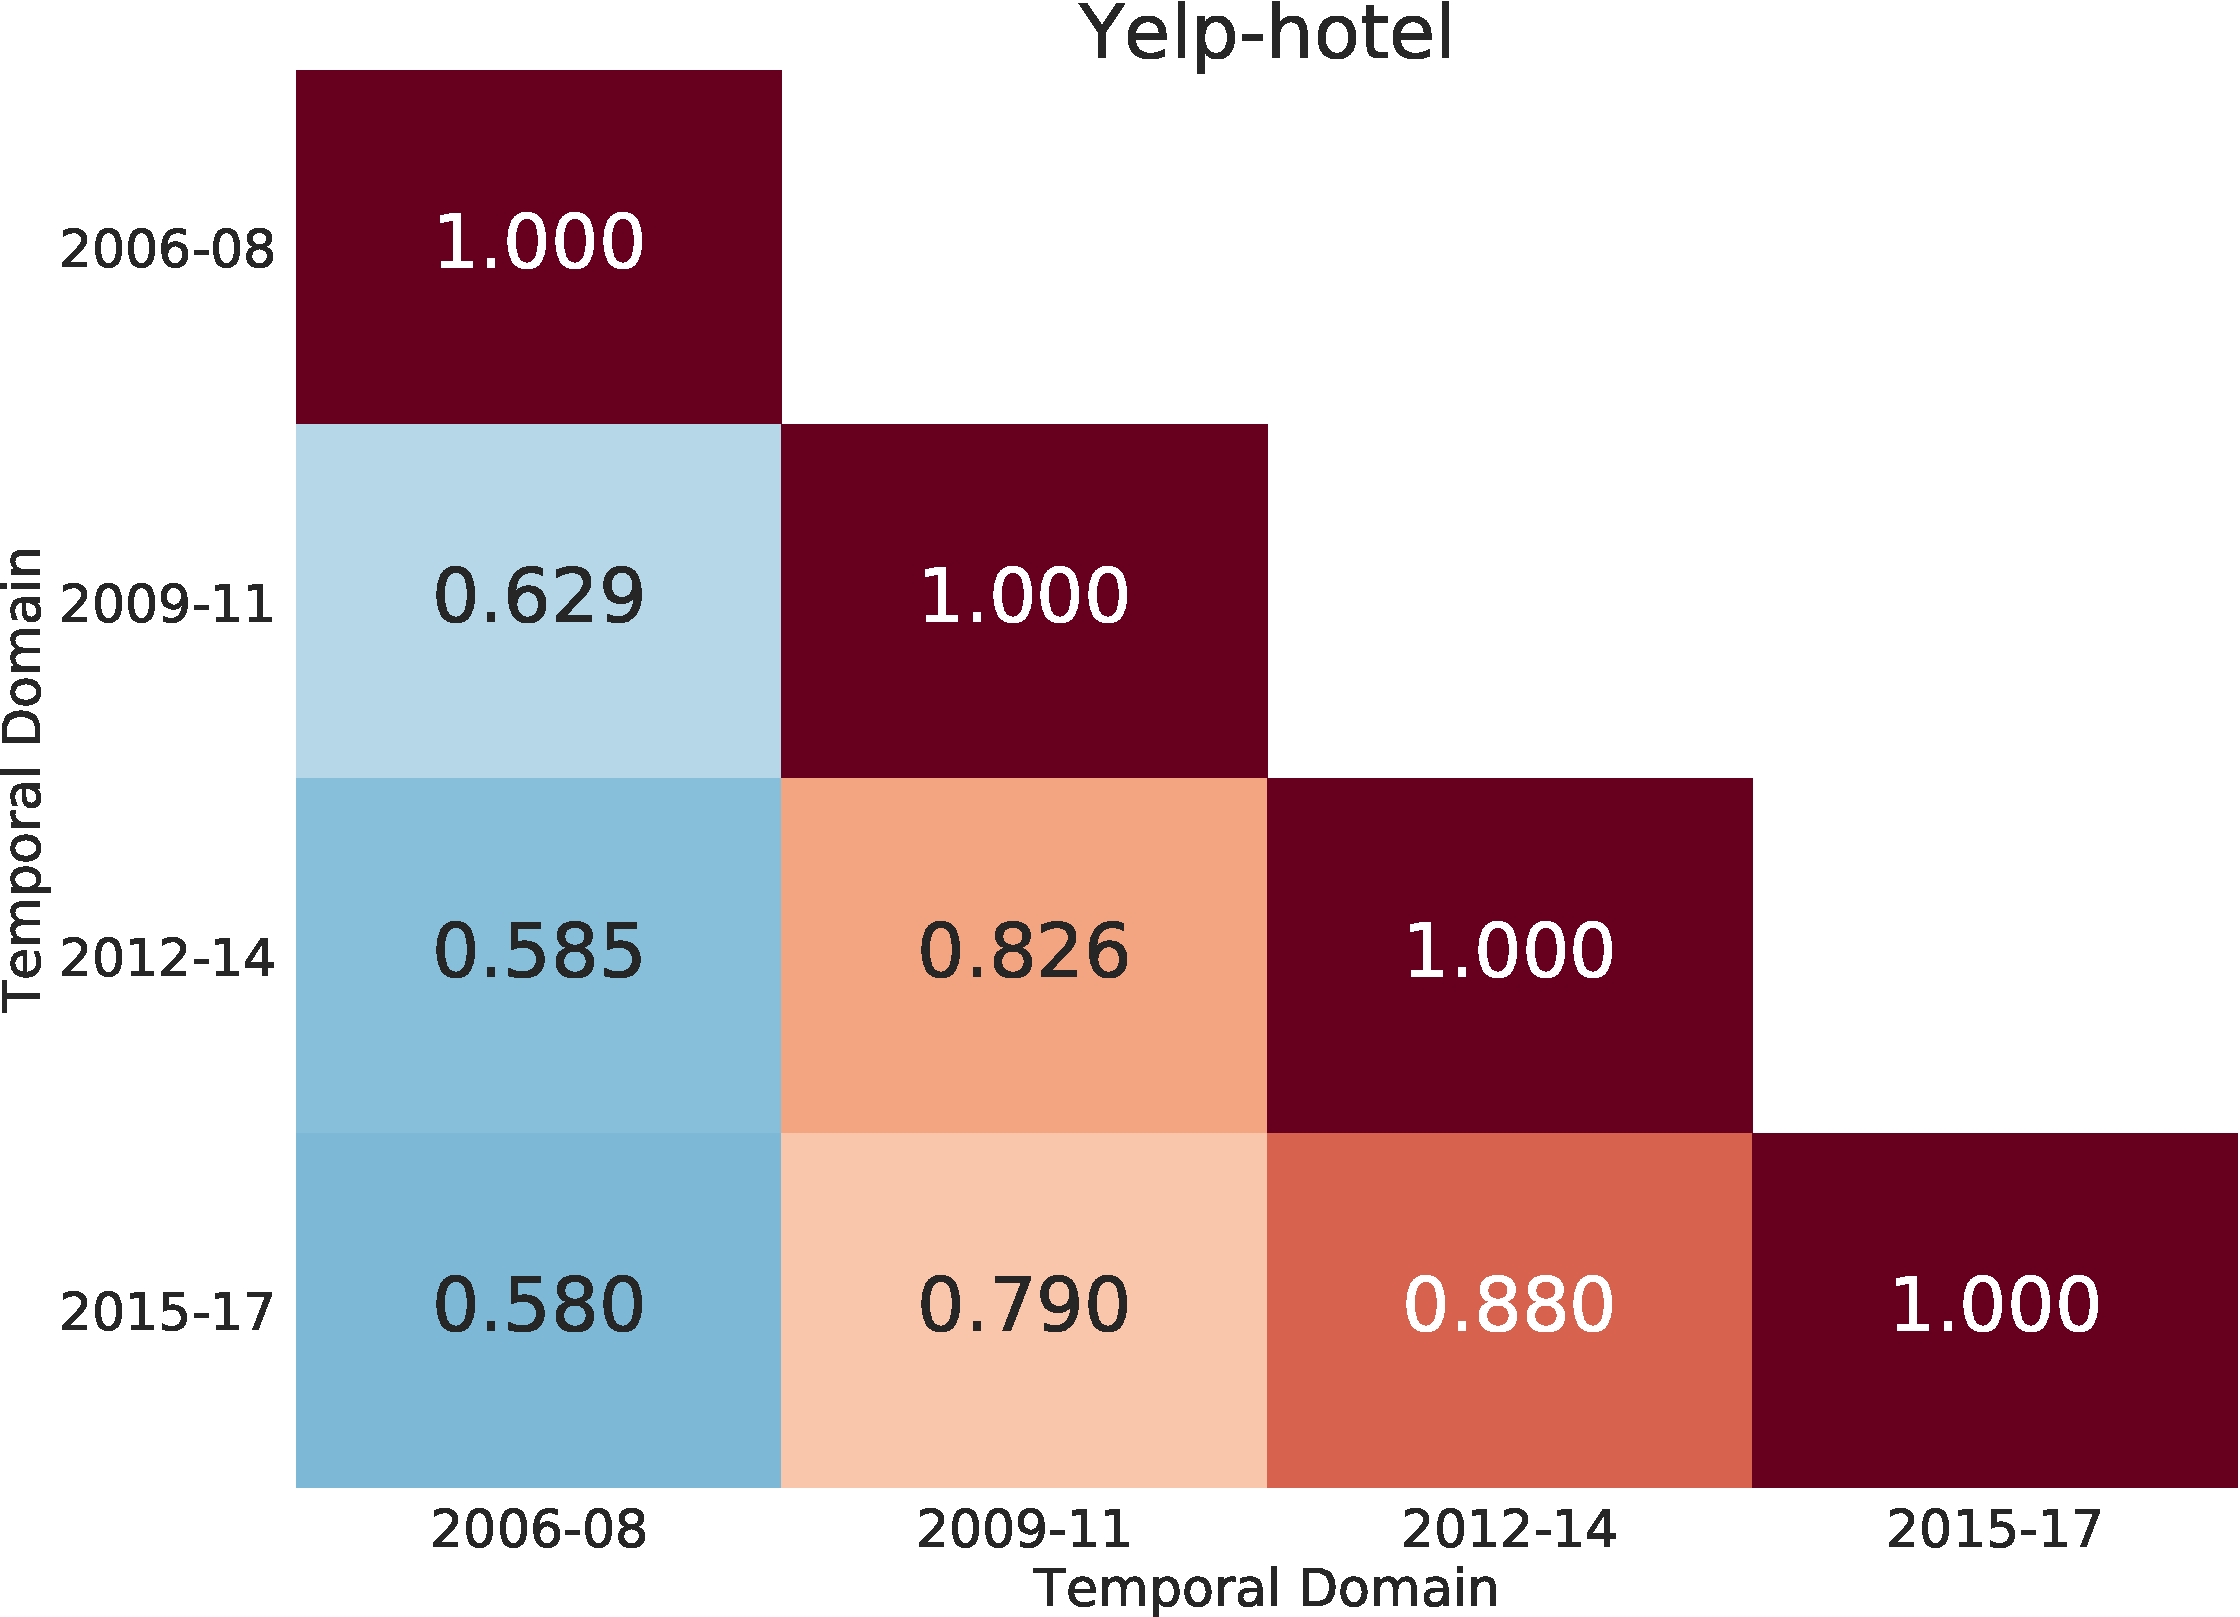
\includegraphics[width=0.32\textwidth]{images/chapter3/lang_use/yelp_hotel.pdf}
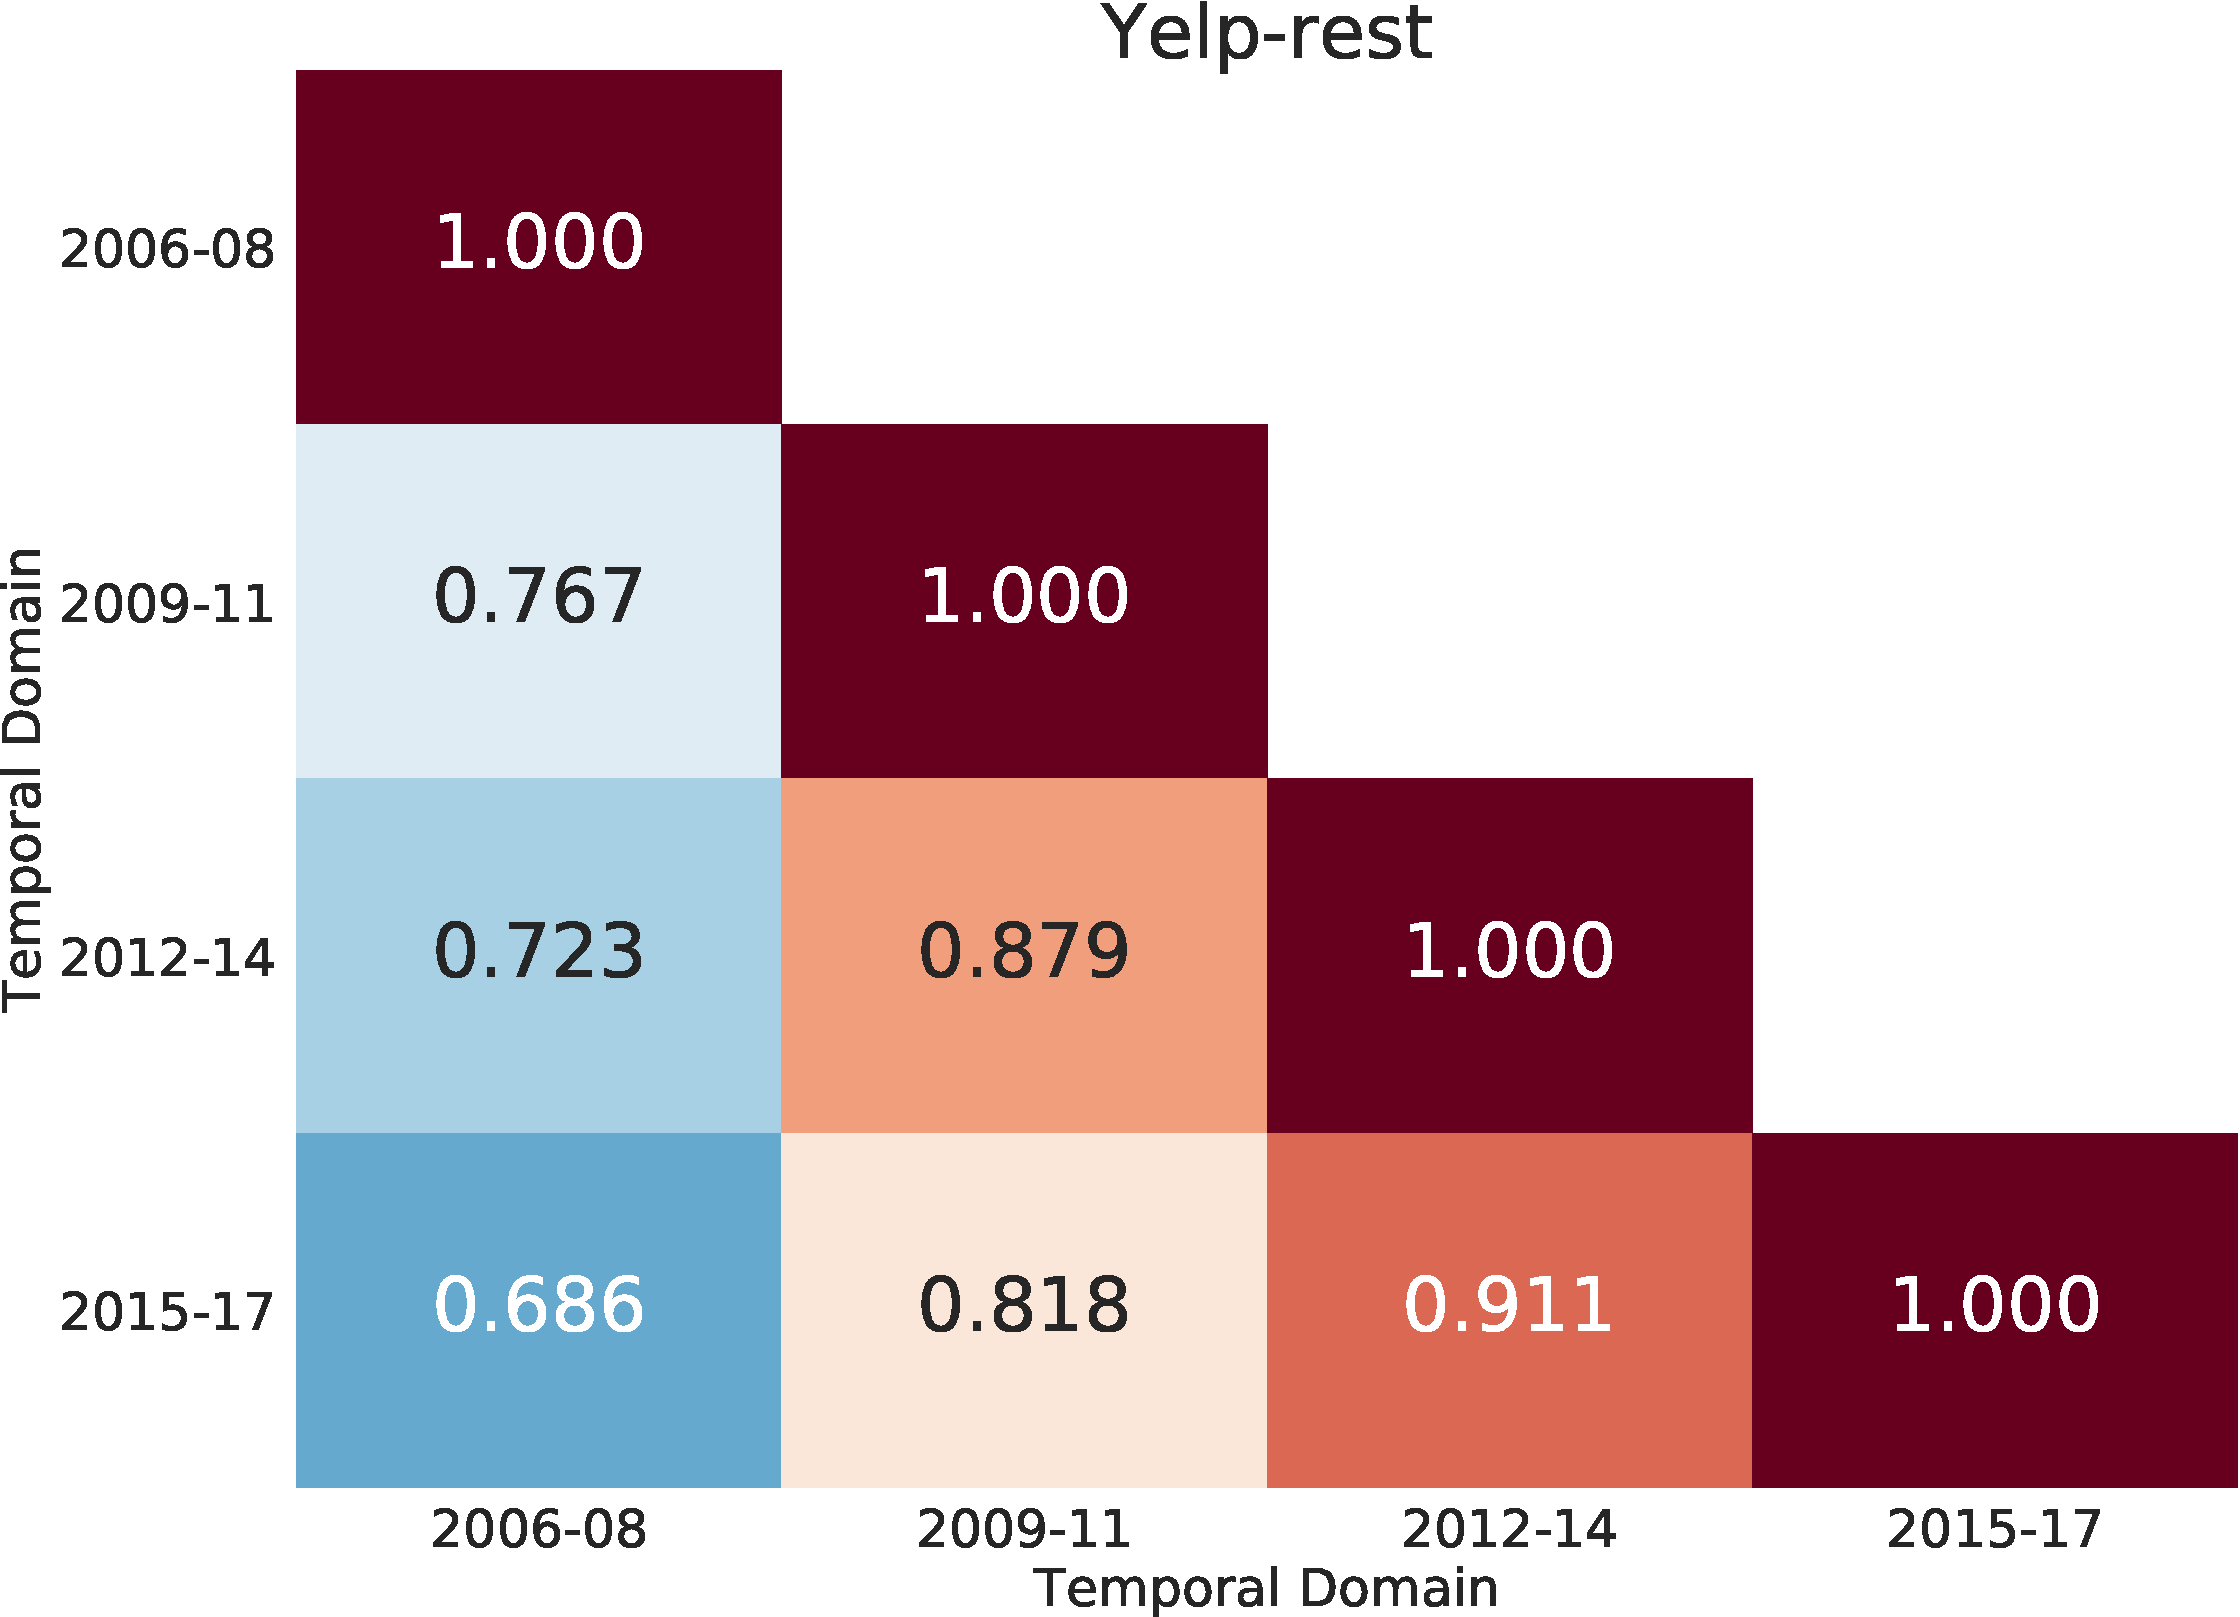
\includegraphics[width=0.32\textwidth]{images/chapter3/lang_use/yelp_rest.pdf}
\caption{Word usage overlaps between every two time domains. A value of 1 means no variations of top features between two temporal domains, while values less than 1 indicate more temporal variations.}
\label{chap3:fig:lang}
\end{figure}

Document classification models often use feature representations that are derived from words. Therefore, variations in word usage across time will change the distribution of features over time, which can impact the stability of document classifiers~\cite{huang2018examining}. 
Our goal in this section is to test whether there are temporal variations in our datasets, how strong the effects are, and what patterns exist of word usage shifts. This will help us understand how word usage variations can affect document classifiers.

We consider word usage as it relates to document classification by measuring the overlap of top word features across time intervals. We rank and select the top 1,000 features for each interval by mutual information. We then calculate the intersection percentage between every two domains; 
specifically, if $S_0$ is the set of top features for one temporal domain and $S_1$ is the set of top features for another attribute, the percent overlap is calculated as $|S_0 \cap S_1|/1000$.

We present the overlaps of word usages across time in Figure~\ref{chap3:fig:lang}.
The overlap of word usage between temporal domains varies greatly across different corpora (ranging from 0.322 to 0.911). We observe that closer temporal domains usually have higher overlap while further temporal domains share less overlap. These results thus suggest that word usage varies over time across many settings.


\subsection{Analysis 2: Context Shift}
\label{chap3:subsec:ctt_shift}

\begin{figure}[tb!]
\centering
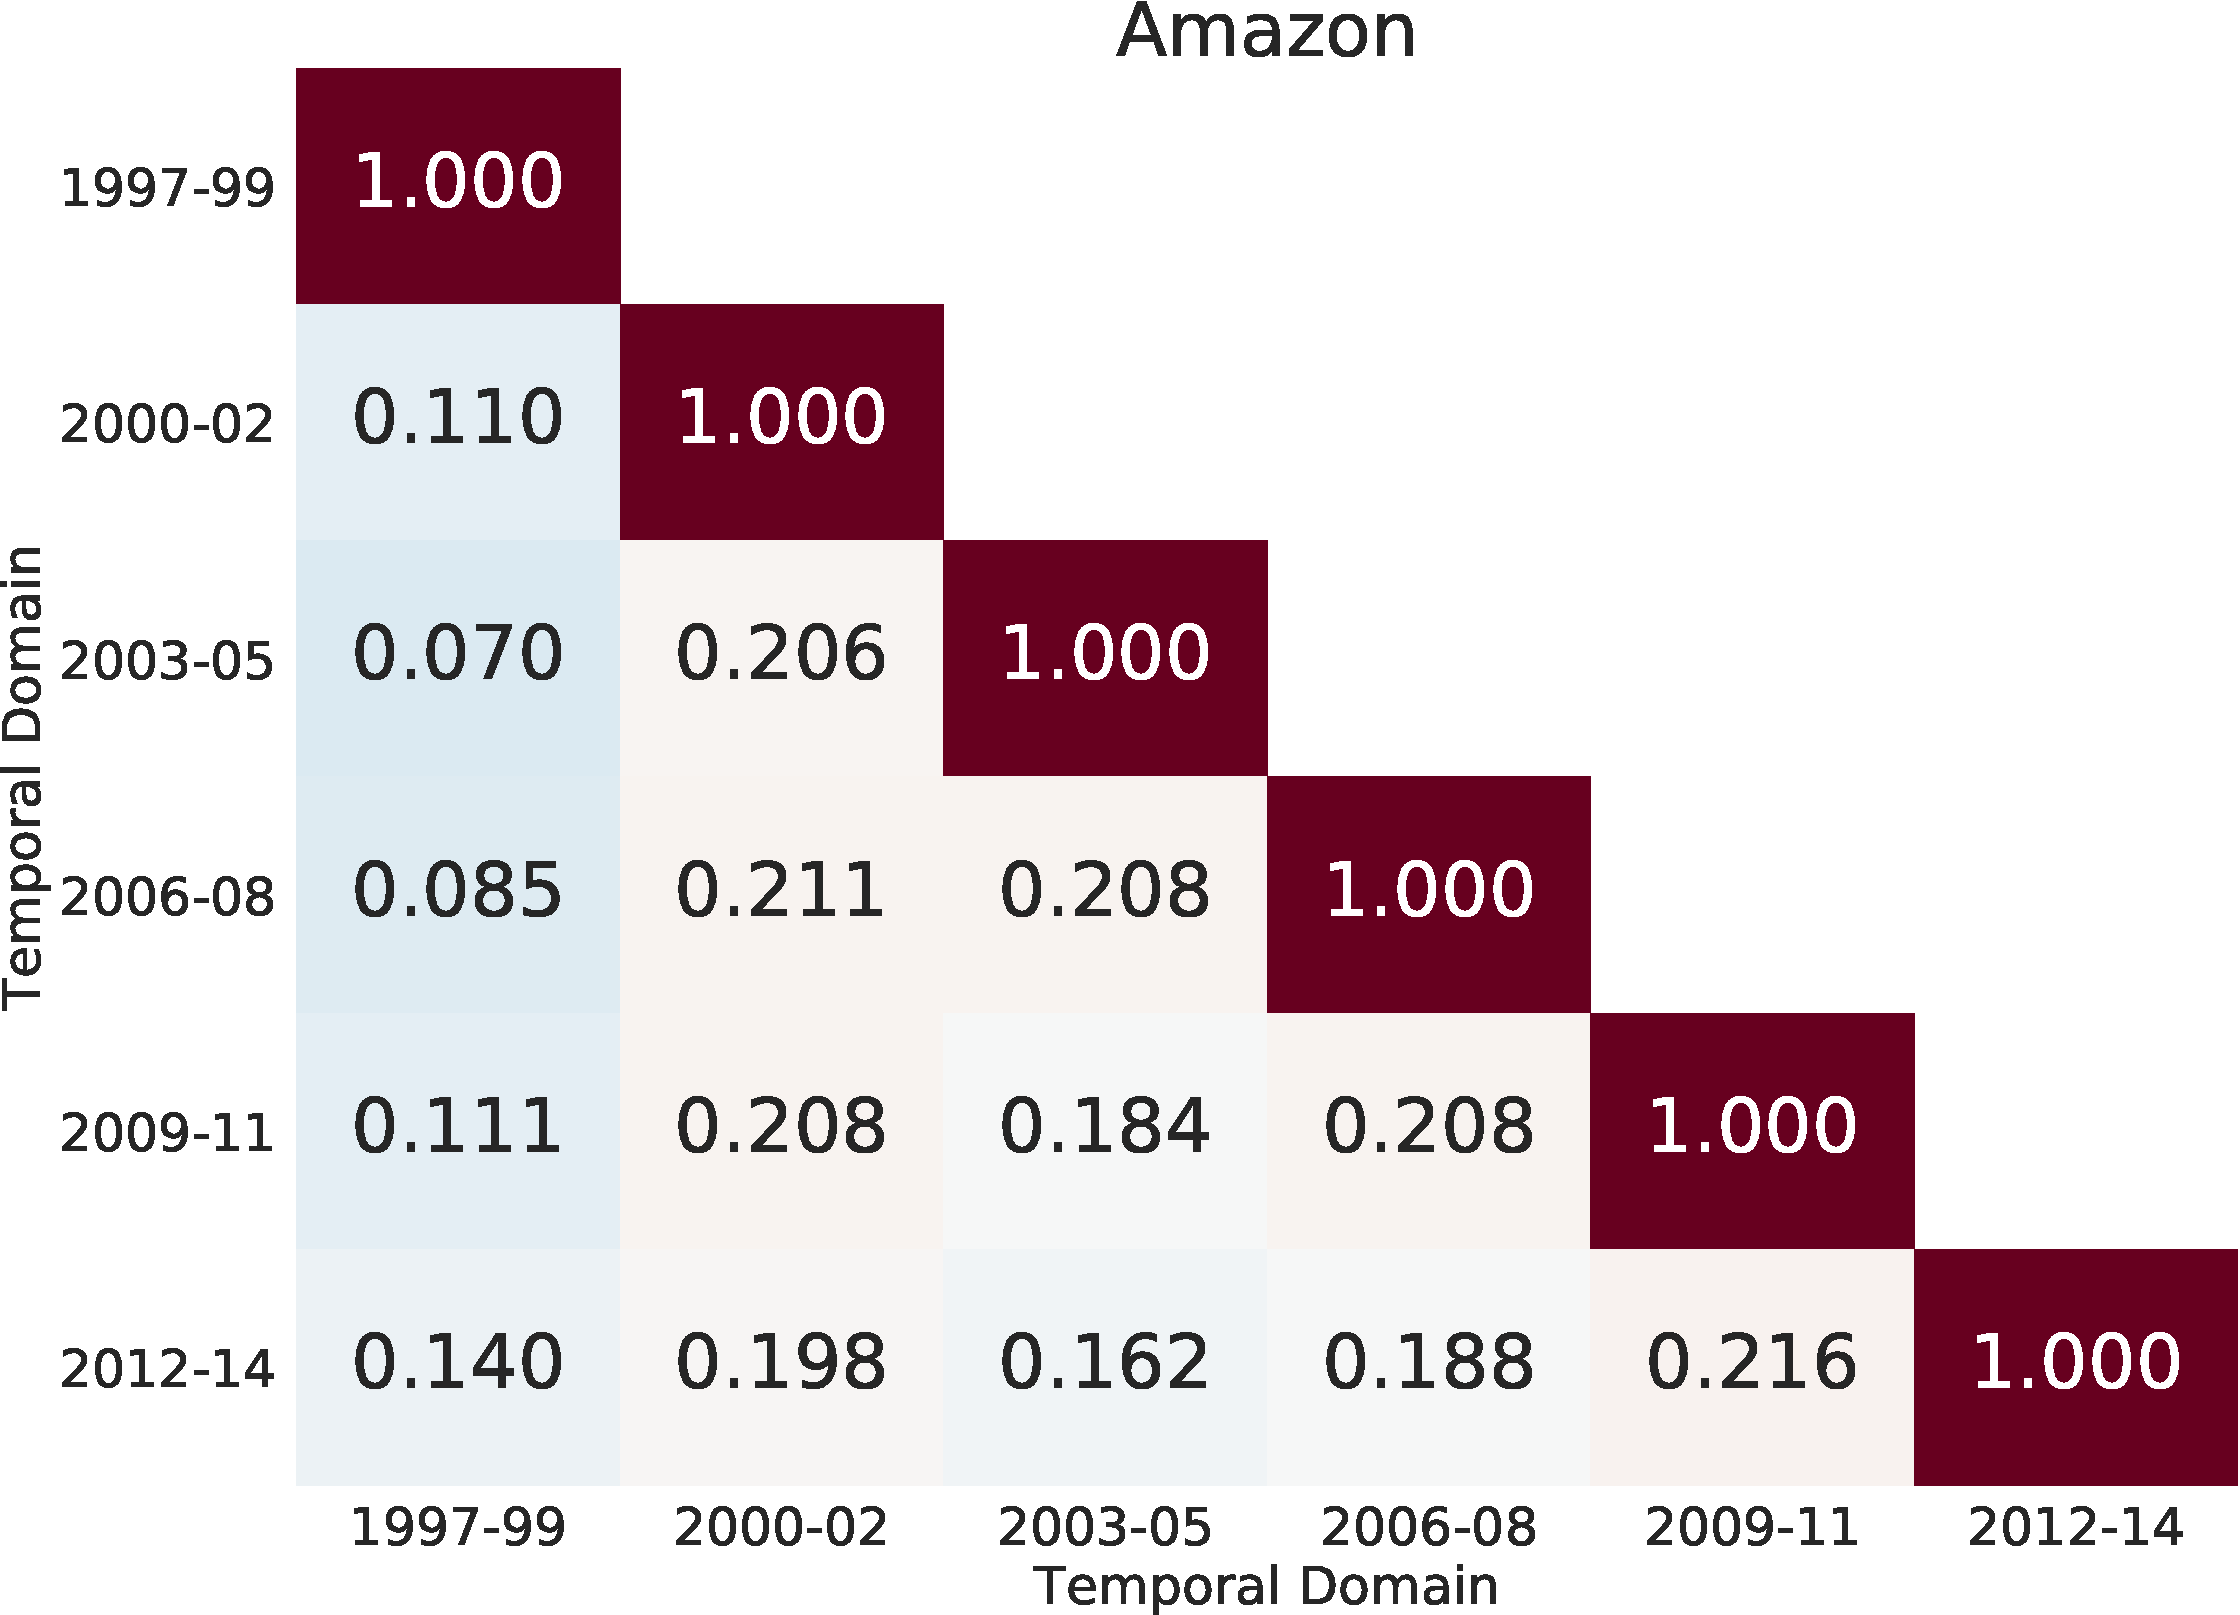
\includegraphics[width=0.32\textwidth]{images/chapter3/ctt_shift/amazon.pdf}
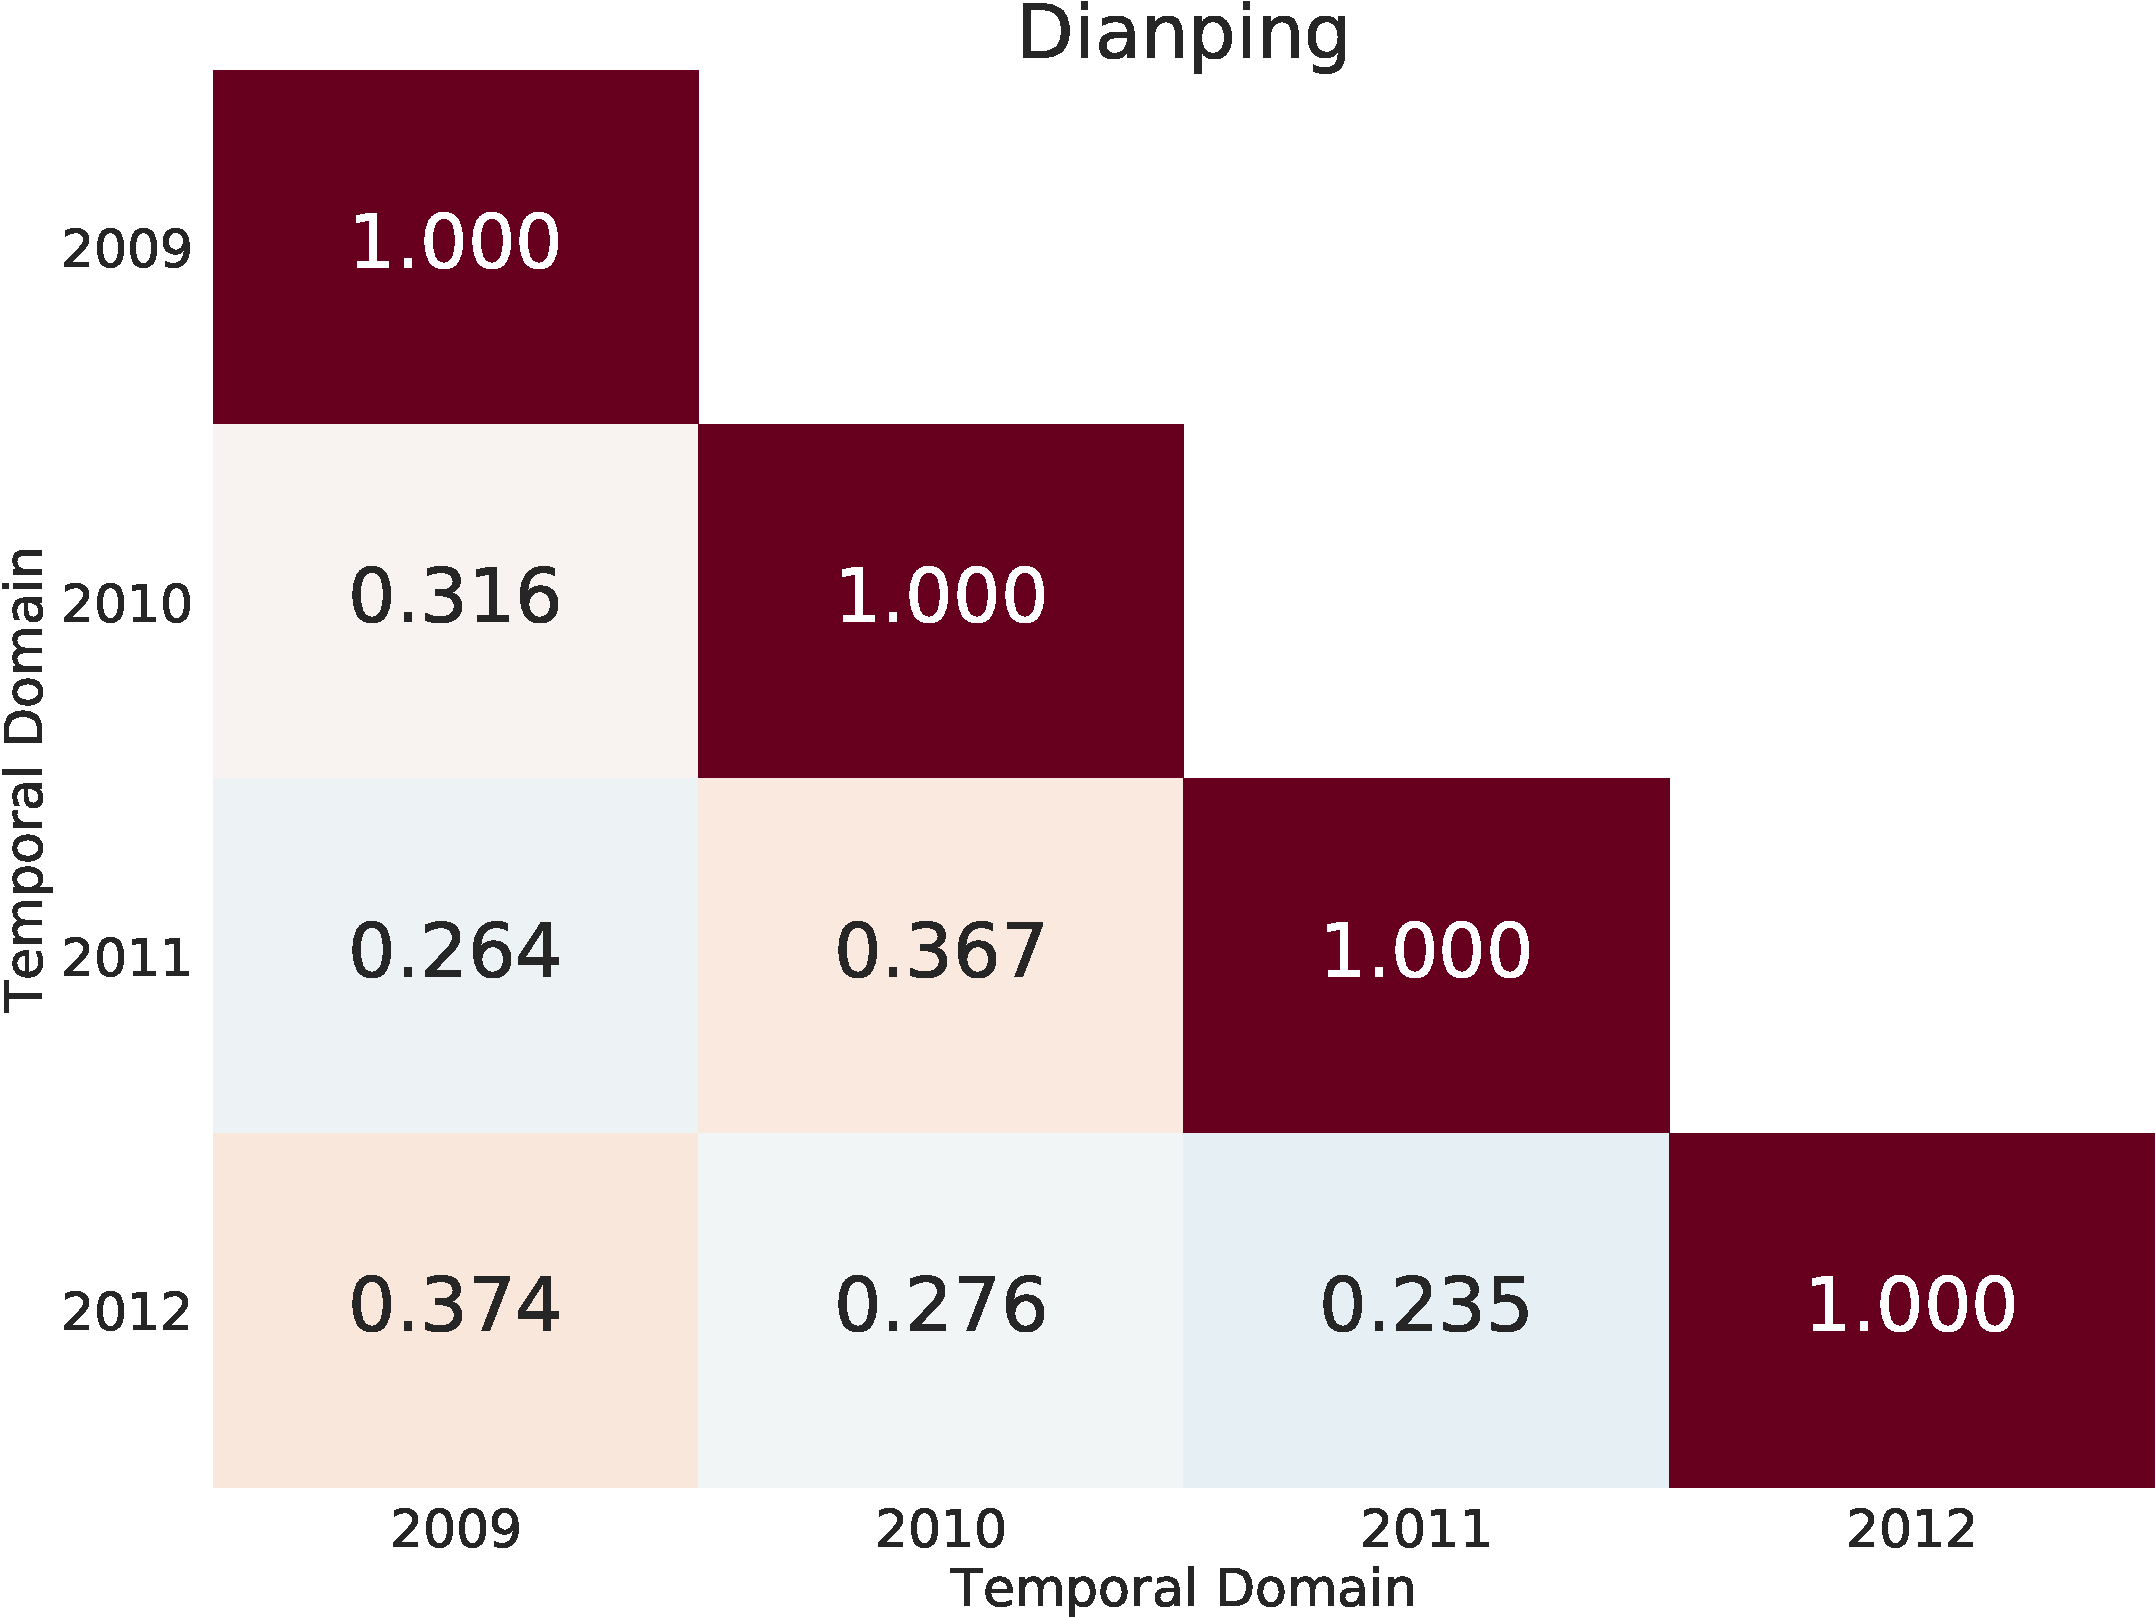
\includegraphics[width=0.32\textwidth]{images/chapter3/ctt_shift/dianping.pdf}
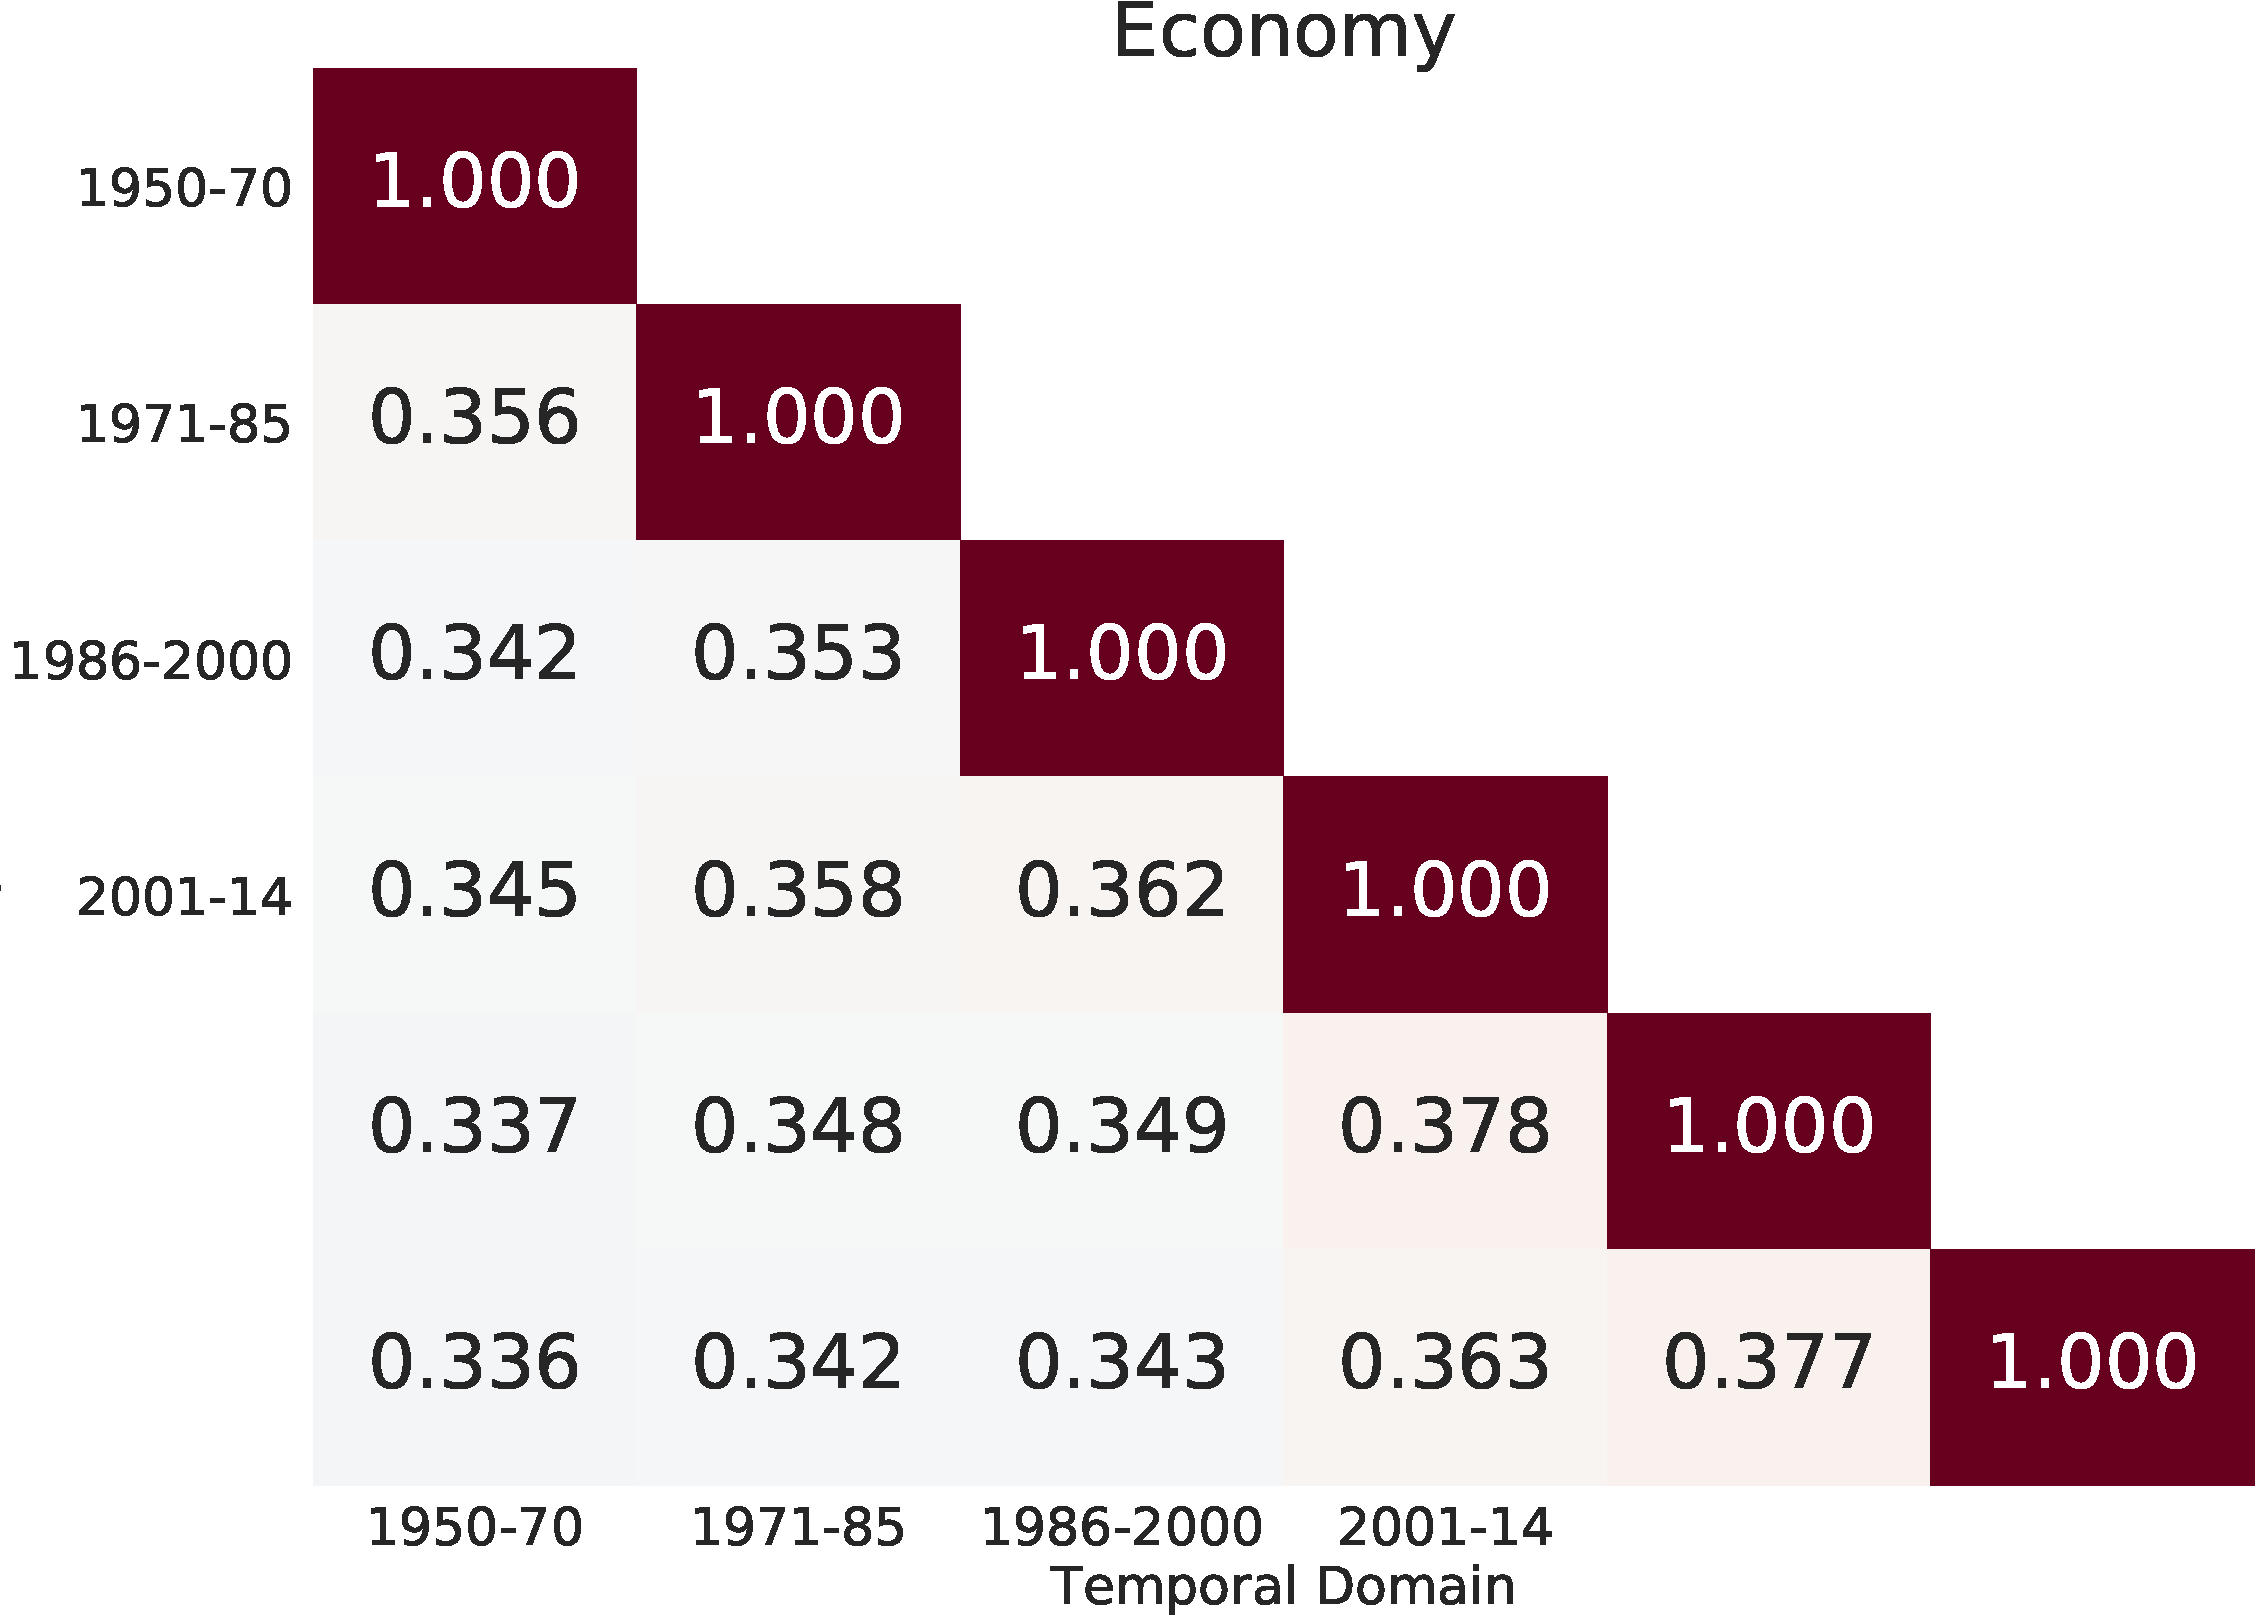
\includegraphics[width=0.32\textwidth]{images/chapter3/ctt_shift/economy.pdf}
\newline
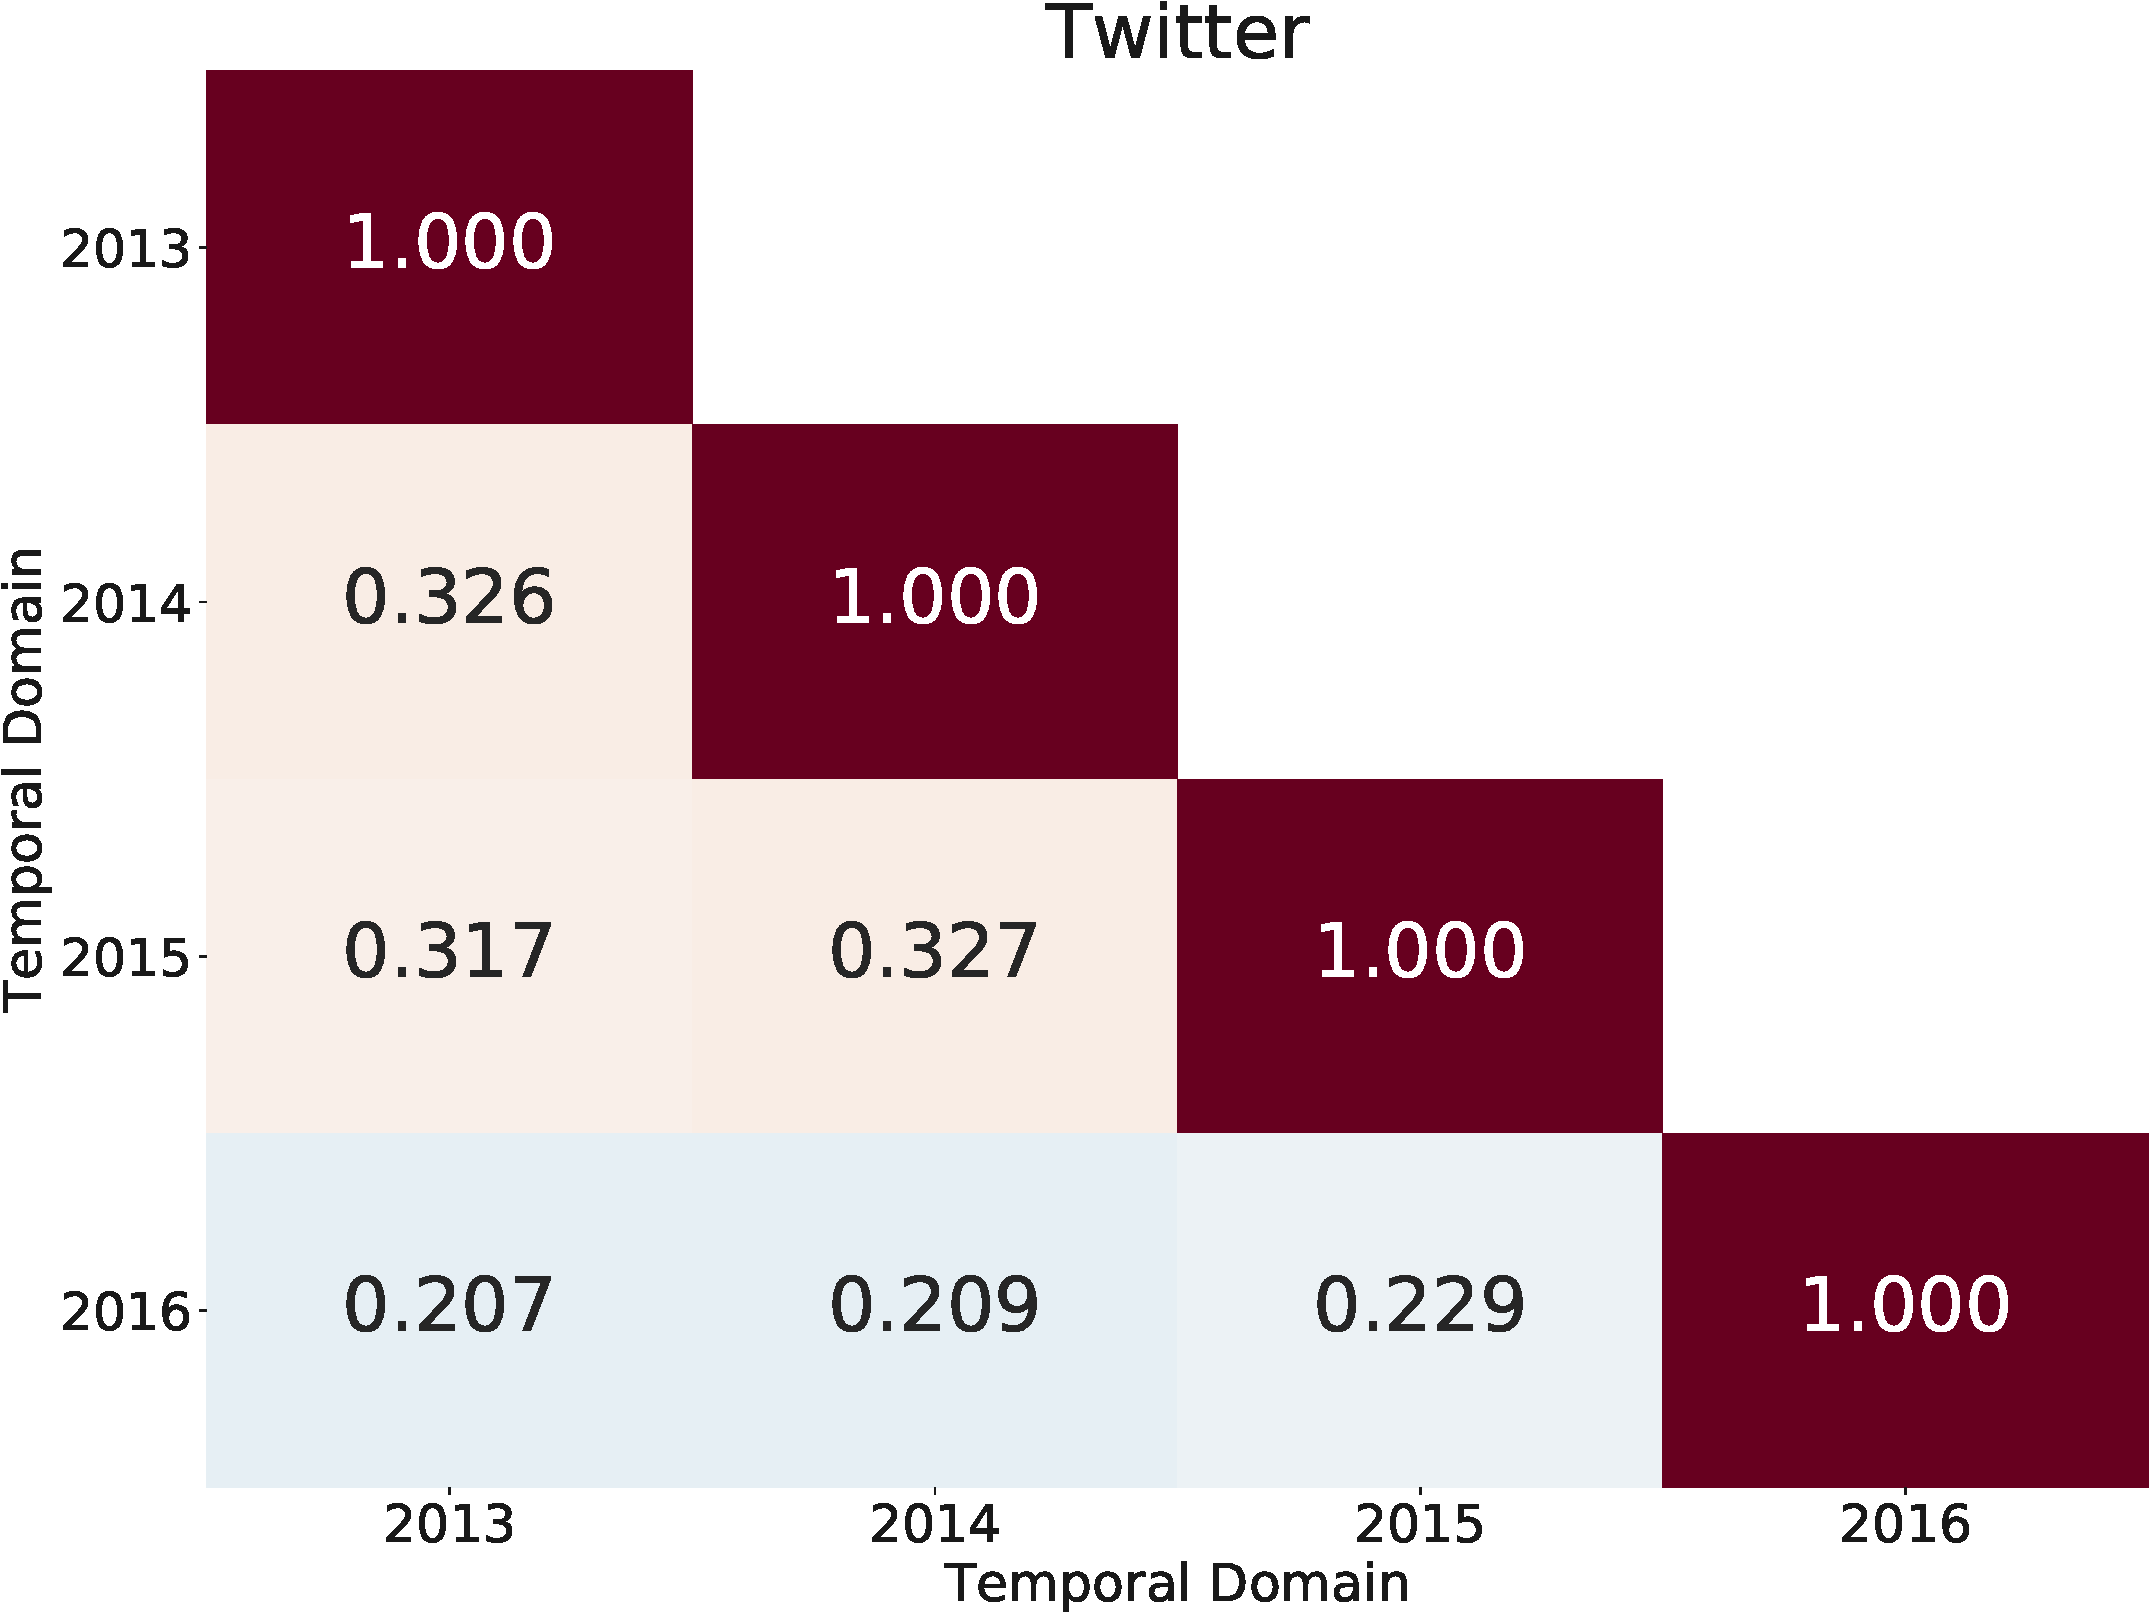
\includegraphics[width=0.32\textwidth]{images/chapter3/ctt_shift/vaccine.pdf}
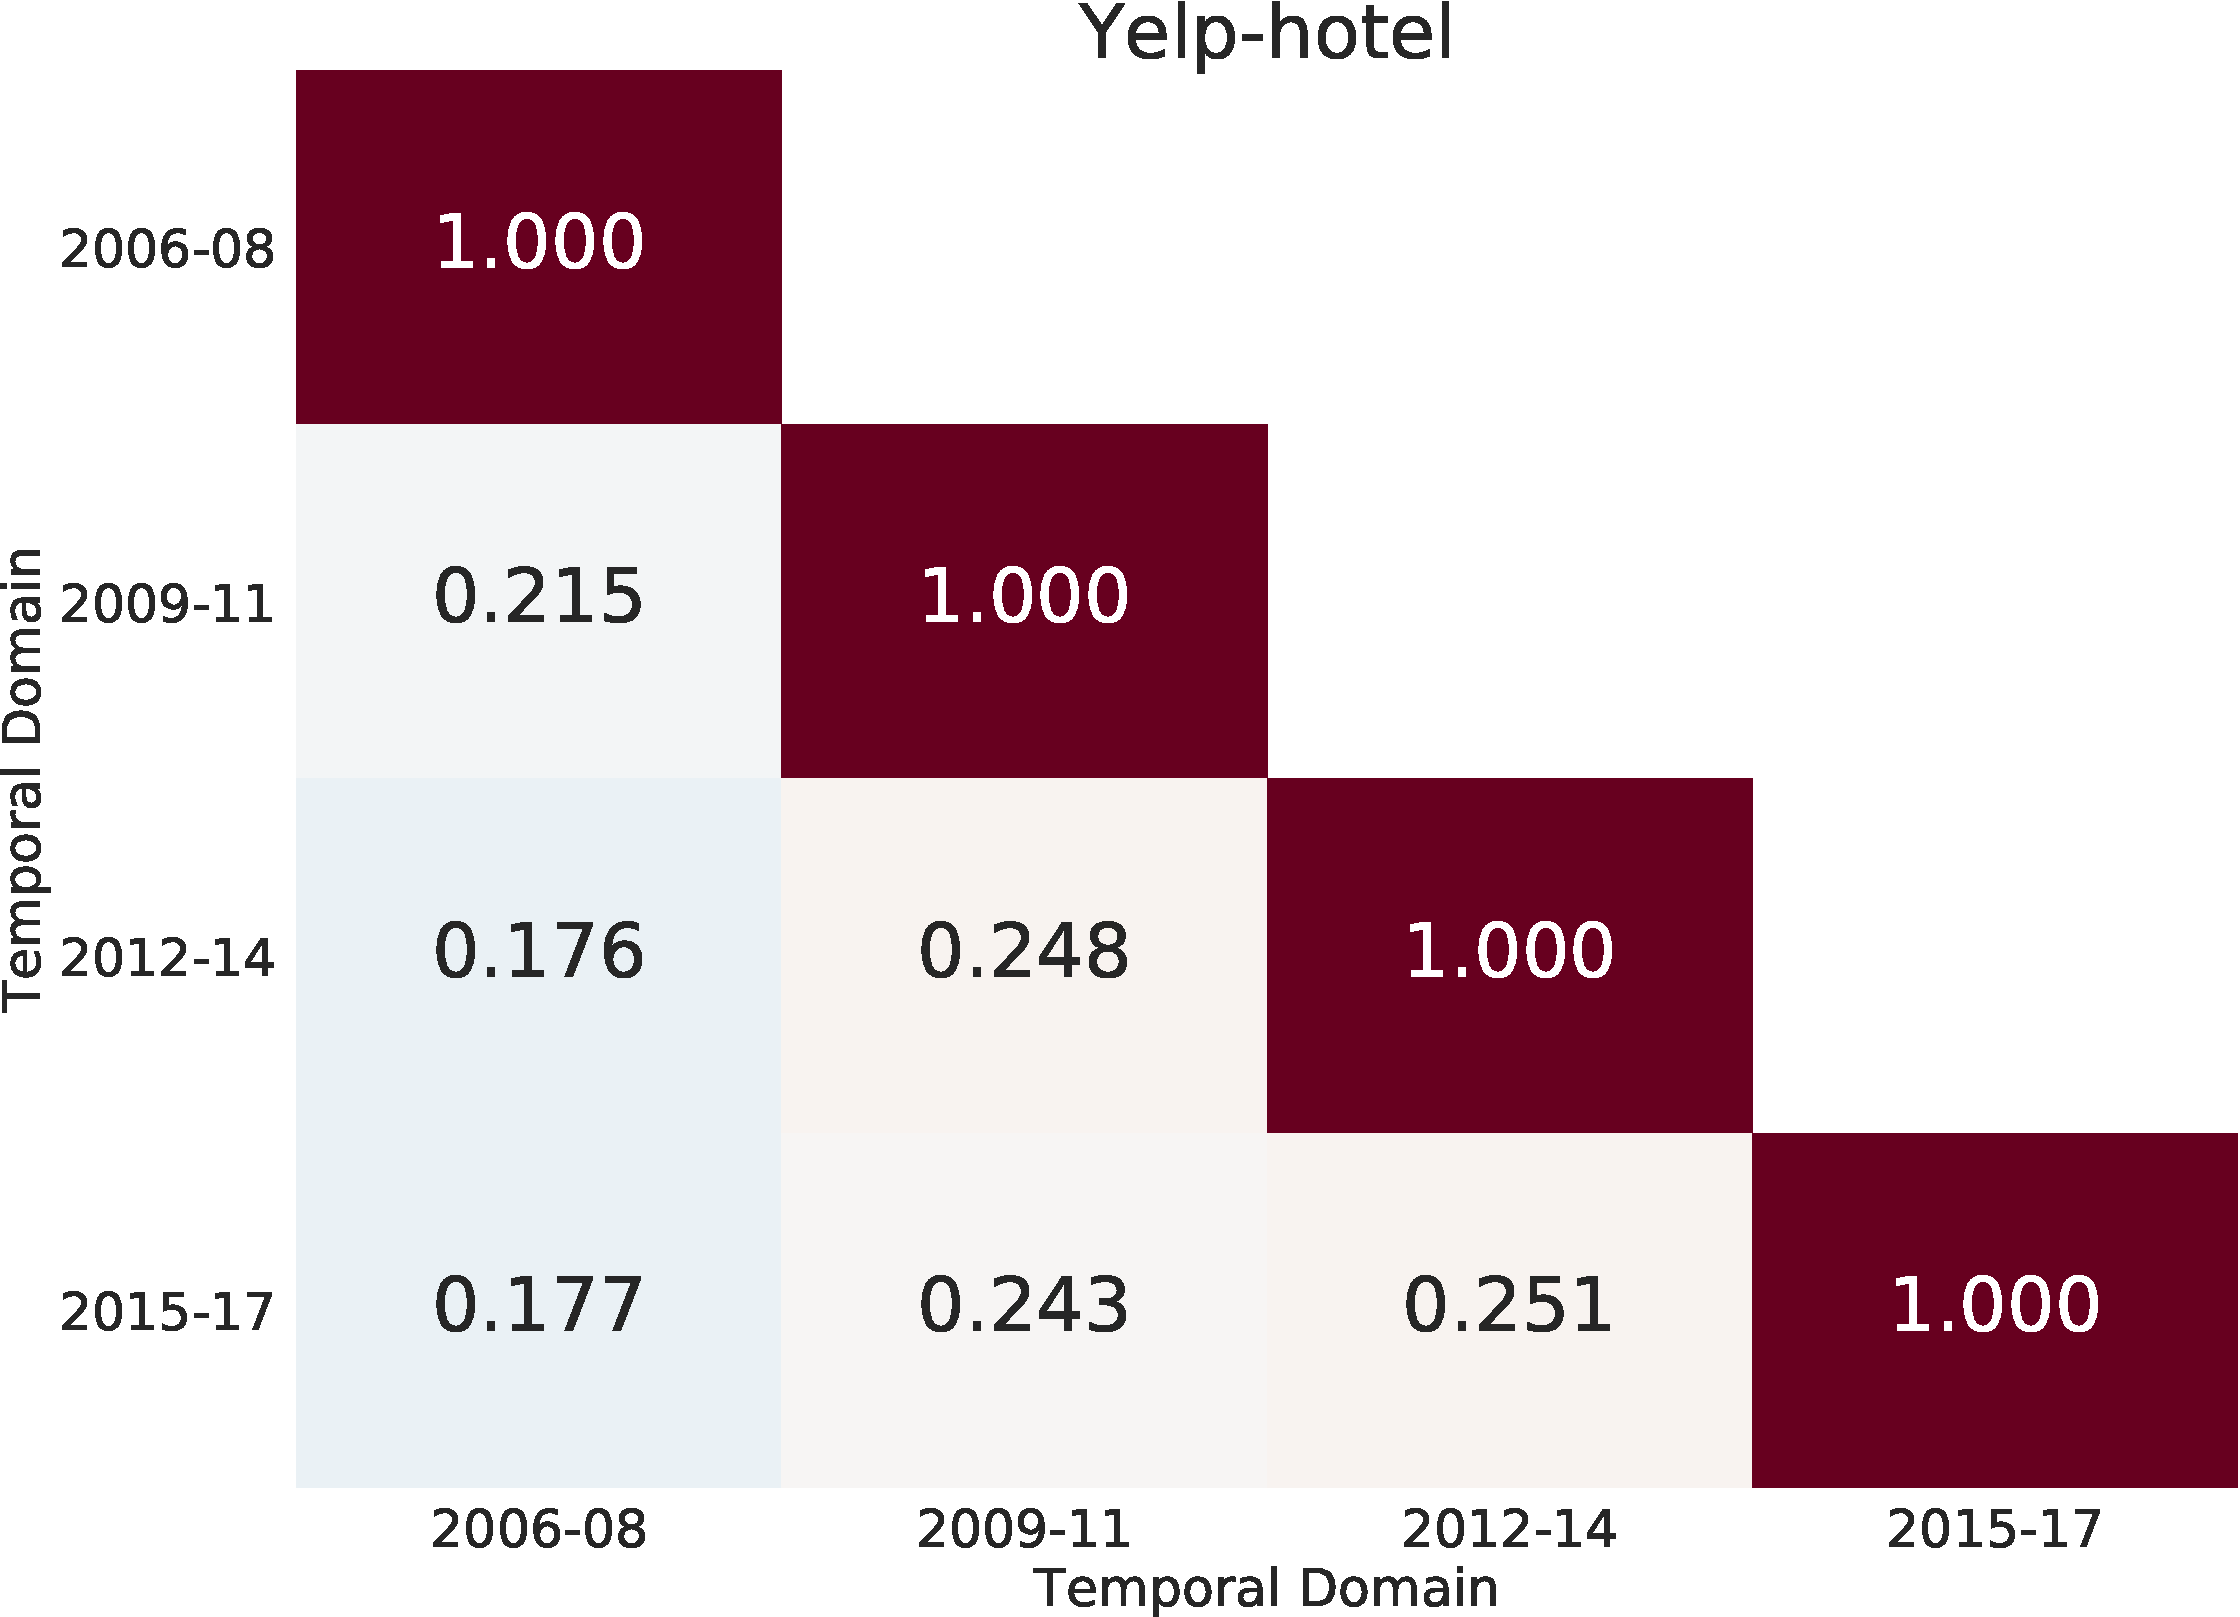
\includegraphics[width=0.32\textwidth]{images/chapter3/ctt_shift/yelp_hotel.pdf}
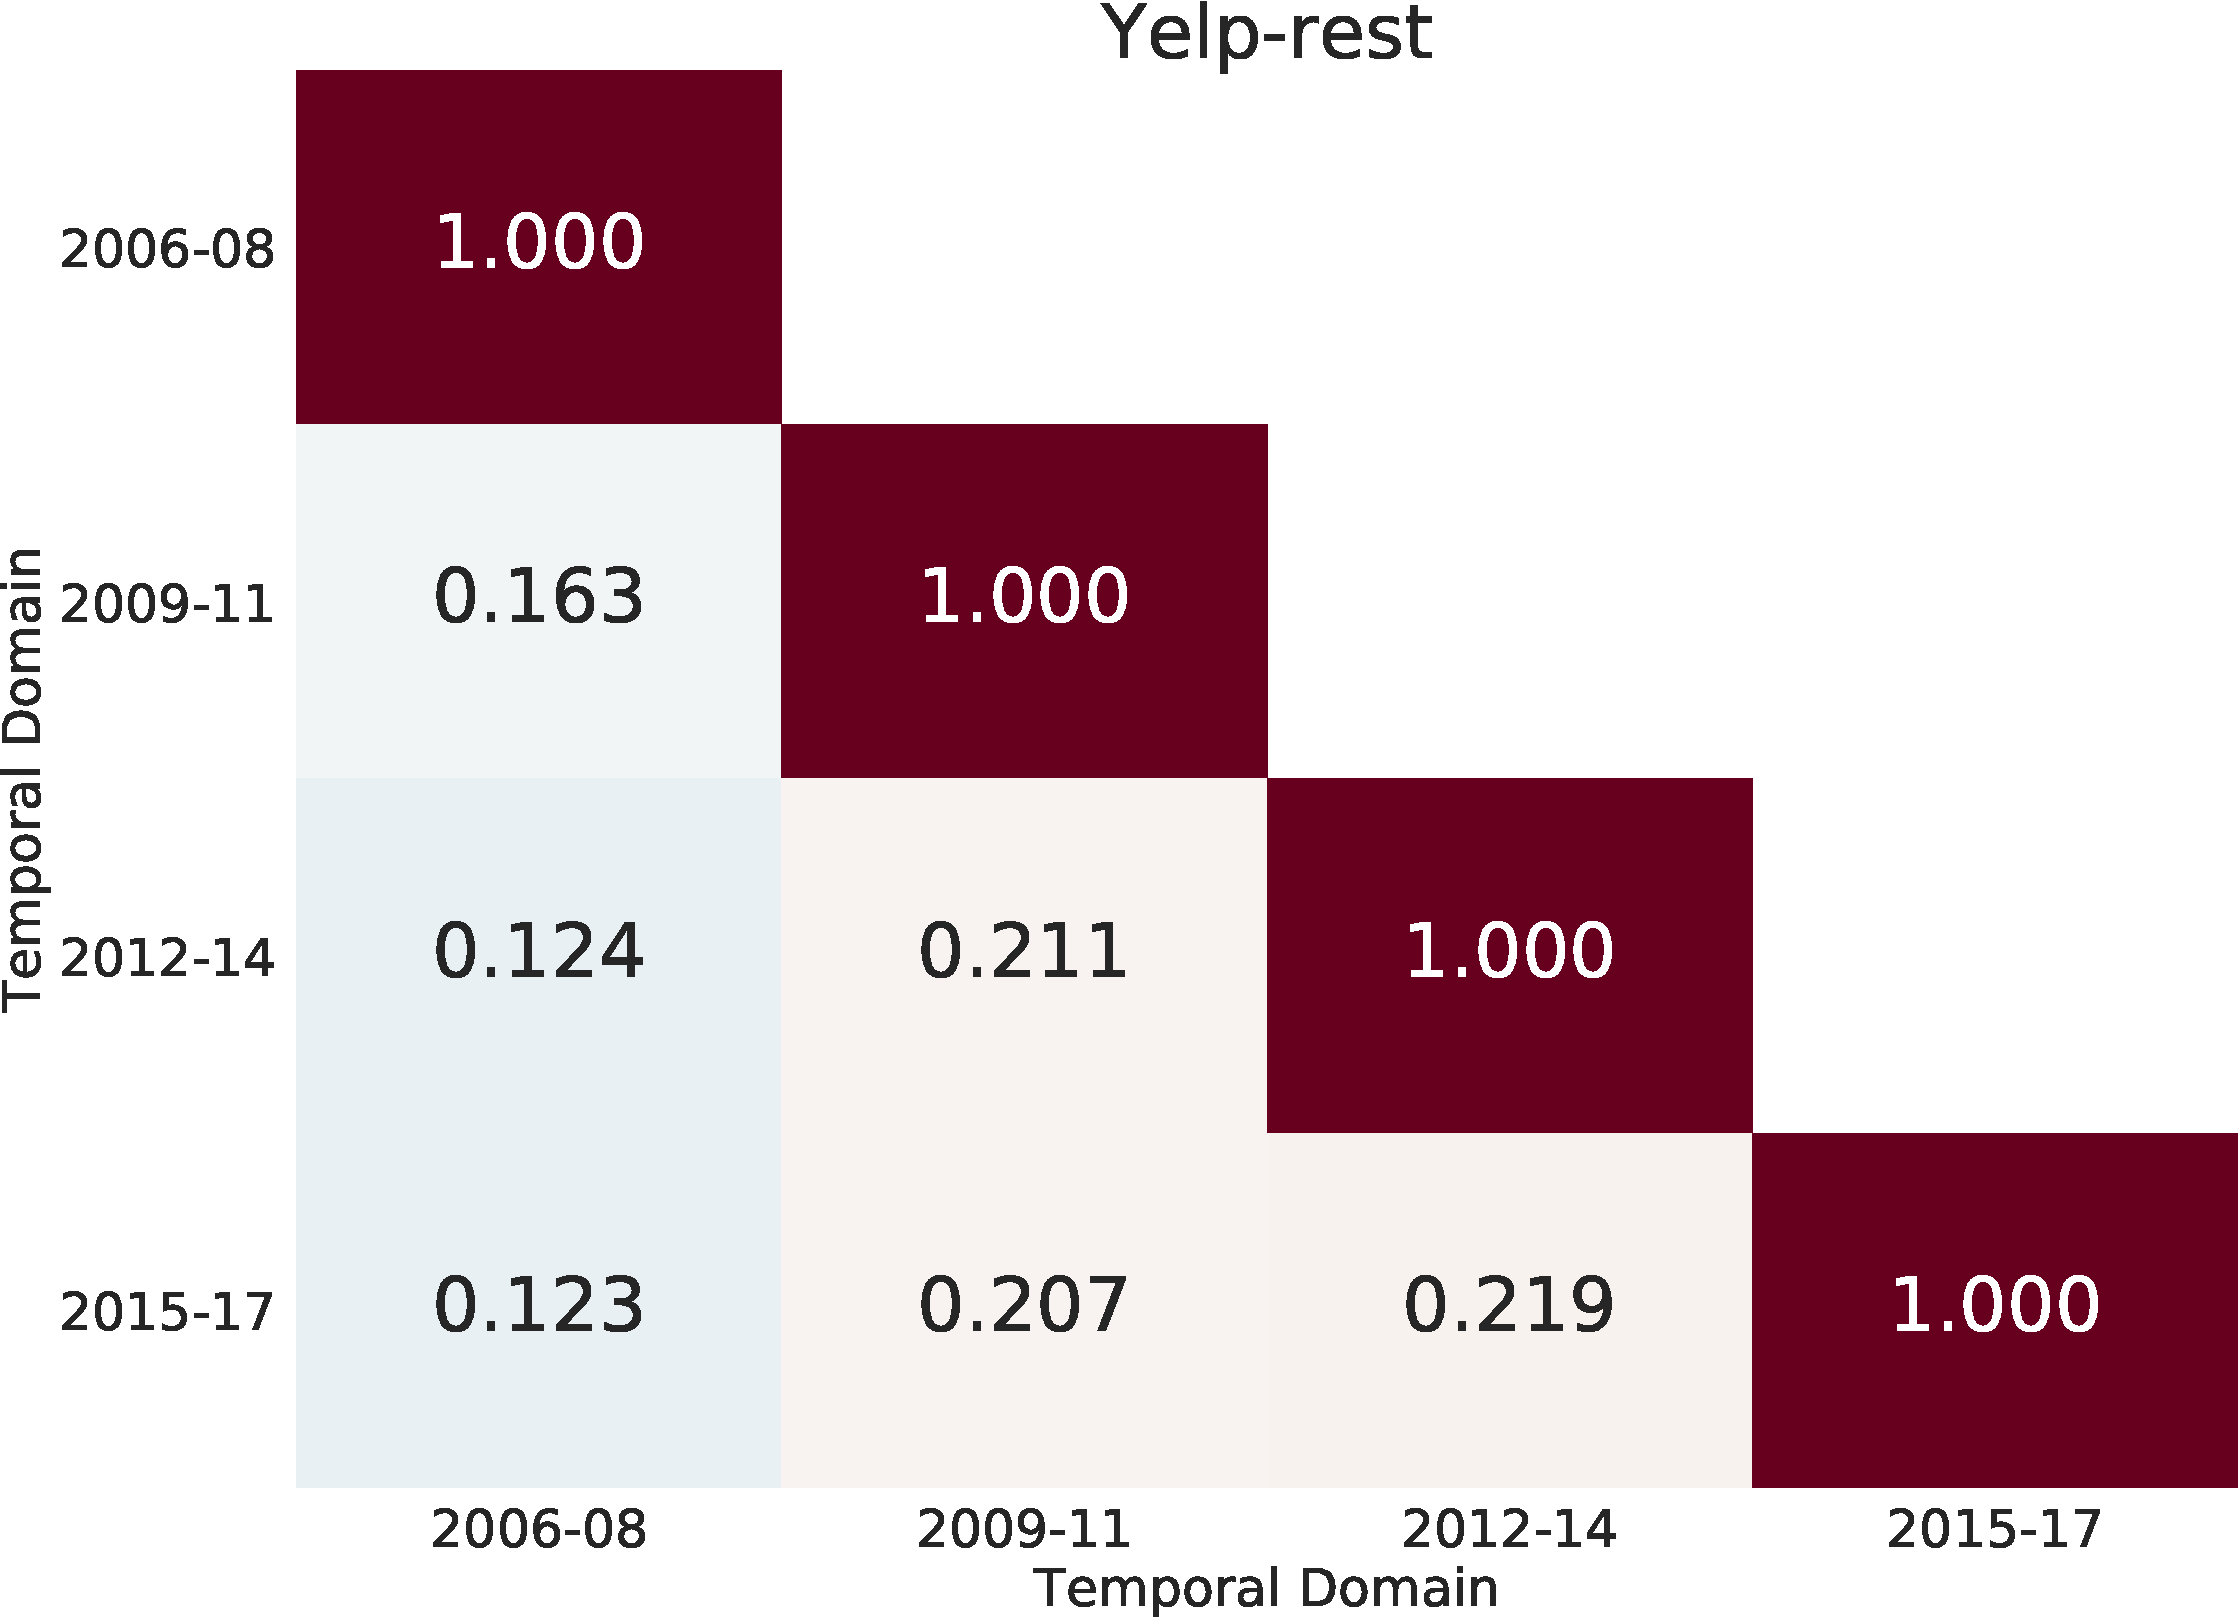
\includegraphics[width=0.32\textwidth]{images/chapter3/ctt_shift/yelp_rest.pdf}
\caption{Context overlaps between every two temporal domains. A value of 0 indicates the contexts of top features between two temporal domains have nothing in common, while values away from 0 mean the contexts share more similarities.}
\label{chap3:fig:ctt}
\end{figure}

Popular word representations for classification train word embeddings using the \textit{context} of each word (a window around the word, e.g., in Skip-gram or CBoW methods)~\cite{mikolov2013distributed, bojanowski2017enriching}.
Contextualized word embedding models such as BERT~\cite{devlin2019bert} use bidirectional contexts to predict masked tokens.
Therefore, we seek to understand how semantic contexts of words shift across time, in addition to the words themselves. 
If we observe a significant context shift, this could lead to inconsistent semantic representations across time.

In the case of context shift, we extract the same unigram features as in the previous section and define word contexts by simulating the word embedding training process via contextual windows. We set a window size of five words and record the words that occur within the context windows. Following the previous section but using the set of words that appear in the context windows, we then calculate the intersection overlap between each pair of time domains.  

We show the overlap in Figure~\ref{chap3:fig:ctt}.
The overlap percentages range from 0.070 to 0.378. We also observe that temporally closer domains share higher percentages of contextual words. The pattern aligns with our observations in the Section~\ref{chap3:subsec:wusage}. 
Since word embeddings rely heavily on contextual information~\cite{mikolov2013distributed, devlin2019bert}, our observations that contexts have little overlap across different time intervals, therefore, suggest it will be important to account for temporality in word embeddings.


\subsection{Analysis 3: Topic Shift}
\label{chap3:subsec:topic}

\begin{figure*}
\centering
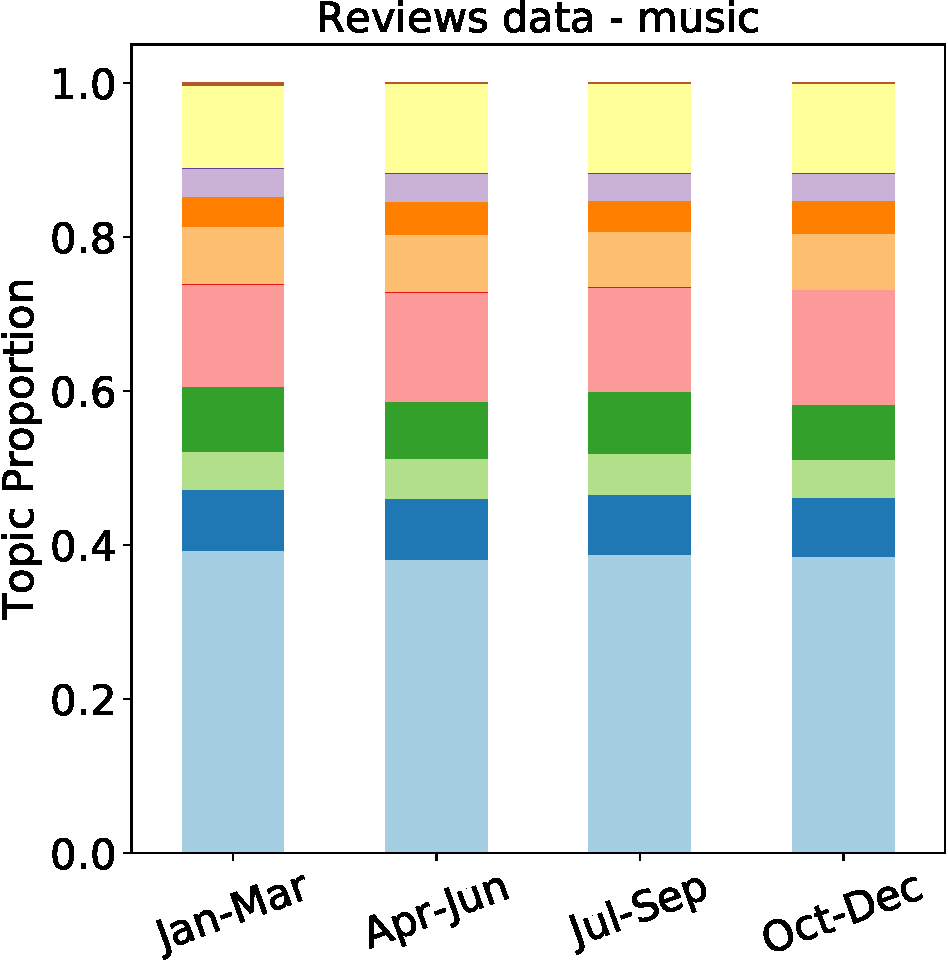
\includegraphics[width=0.235\textwidth]{images/chapter3/acl2018/topic_amazon_month.pdf}
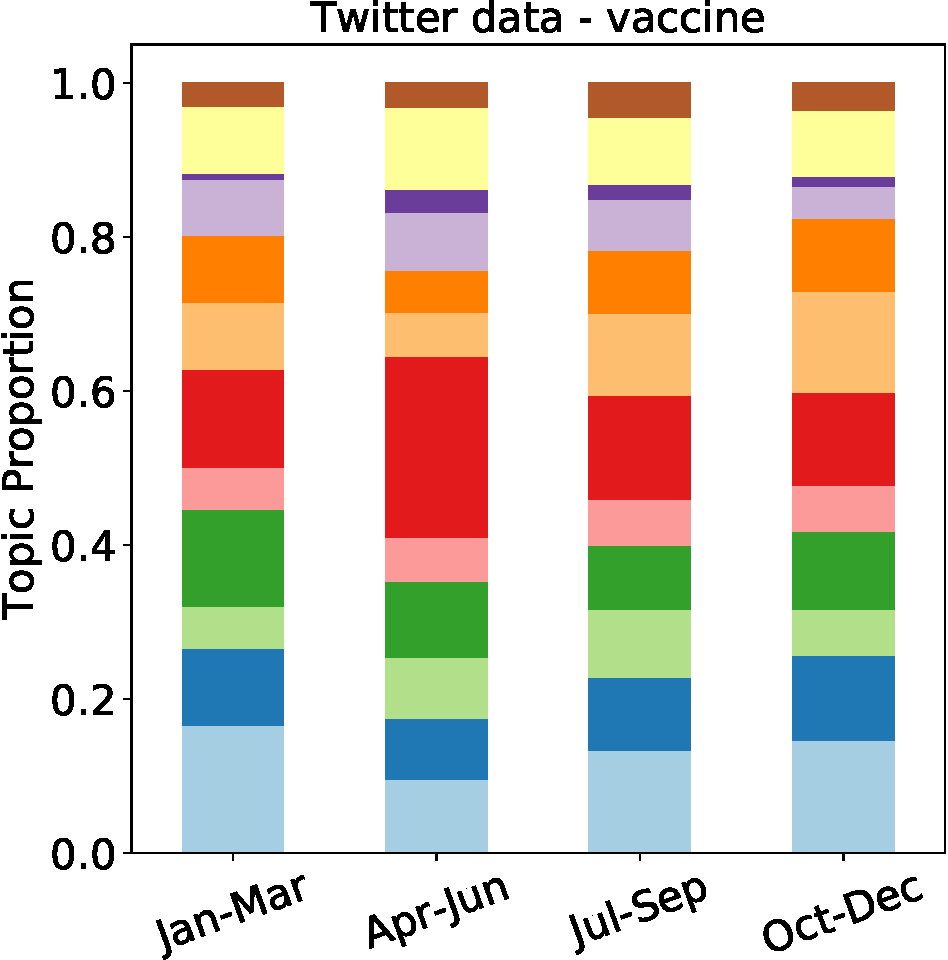
\includegraphics[width=0.235\textwidth]{images/chapter3/acl2018/topic_vaccine_month.pdf} 
\quad
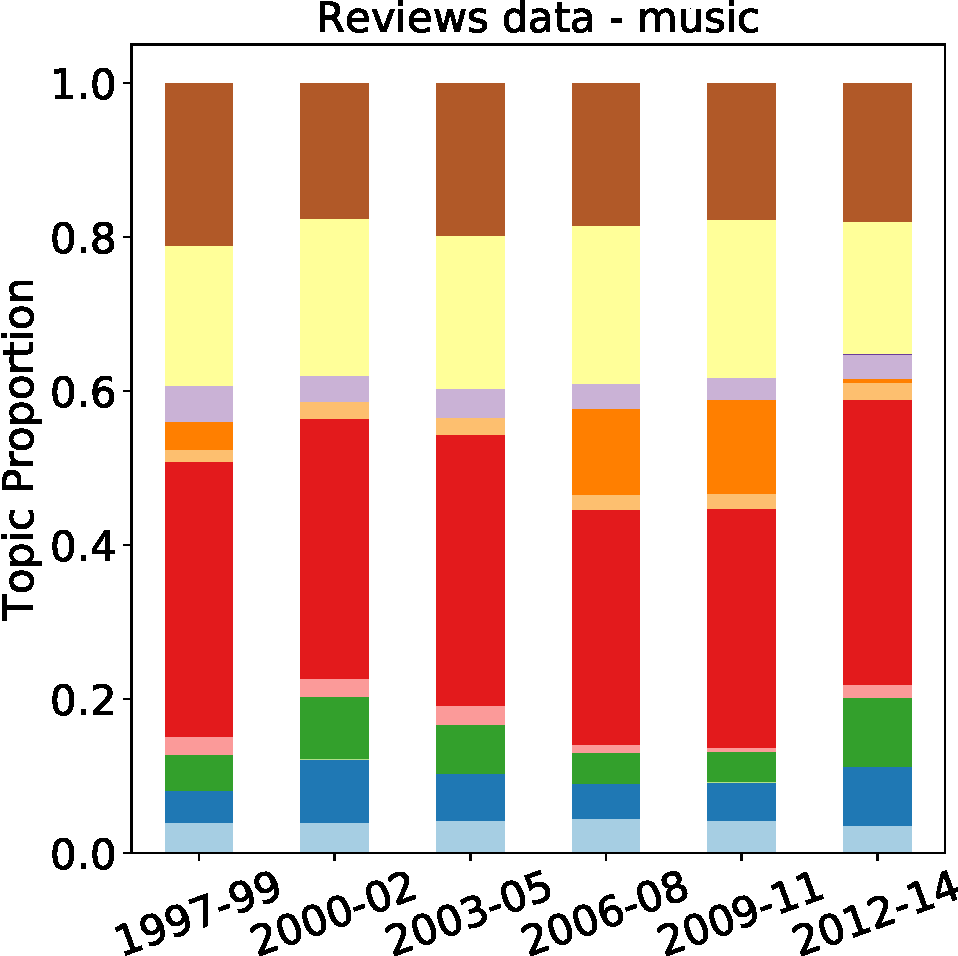
\includegraphics[width=0.235\textwidth]{images/chapter3/acl2018/topic_amazon_year.pdf}
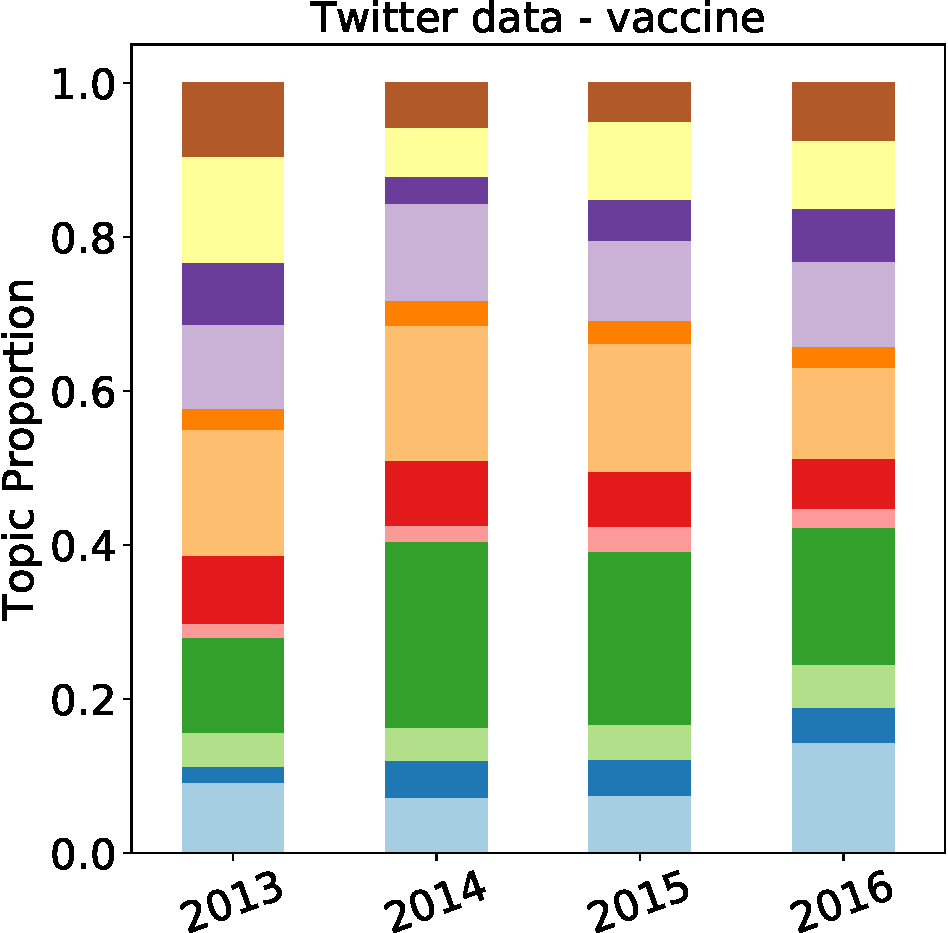
\includegraphics[width=0.235\textwidth]{images/chapter3/acl2018/topic_vaccine_year.pdf}
\caption{\label{chap3:fig:topic} Topic distributions in each time of year (left) and each span of years (right). Topic models are trained independently in the seasonal vs. non-seasonal settings and are not aligned. The music and vaccine refer to Amazon and Twitter datasets respectively.}
\end{figure*}

Finally, to understand why performance varies, we also qualitatively examined how the distribution of content changes across time intervals.
To measure the distribution of content, we trained a topic model with 20 topics using \texttt{Gensim}~\cite{rehurek2010software} with default parameters.
We associated each document with one topic (the most probable topic in the document) and then calculated the proportion of each topic within a period as the proportion of documents in that period assigned to that topic.
We can then visualize the extent to which the distribution of 20 topics varies by time.

Figure~\ref{chap3:fig:topic} (left) shows the distribution of topics in each seasonal interval for two corpora: Amazon music reviews and Twitter.
We observe very little variation in the topic distribution across seasons while some changes across non-seasonal intervals in the Amazon corpus, but more variations in the Twitter corpus, which may explain the large performance differences when testing on held-out seasons in the Twitter data as compared to the Amazon corpus.


\subsection{Analysis 4: Impacts on Document Classifiers}

\begin{figure*}[tb!]
\centering
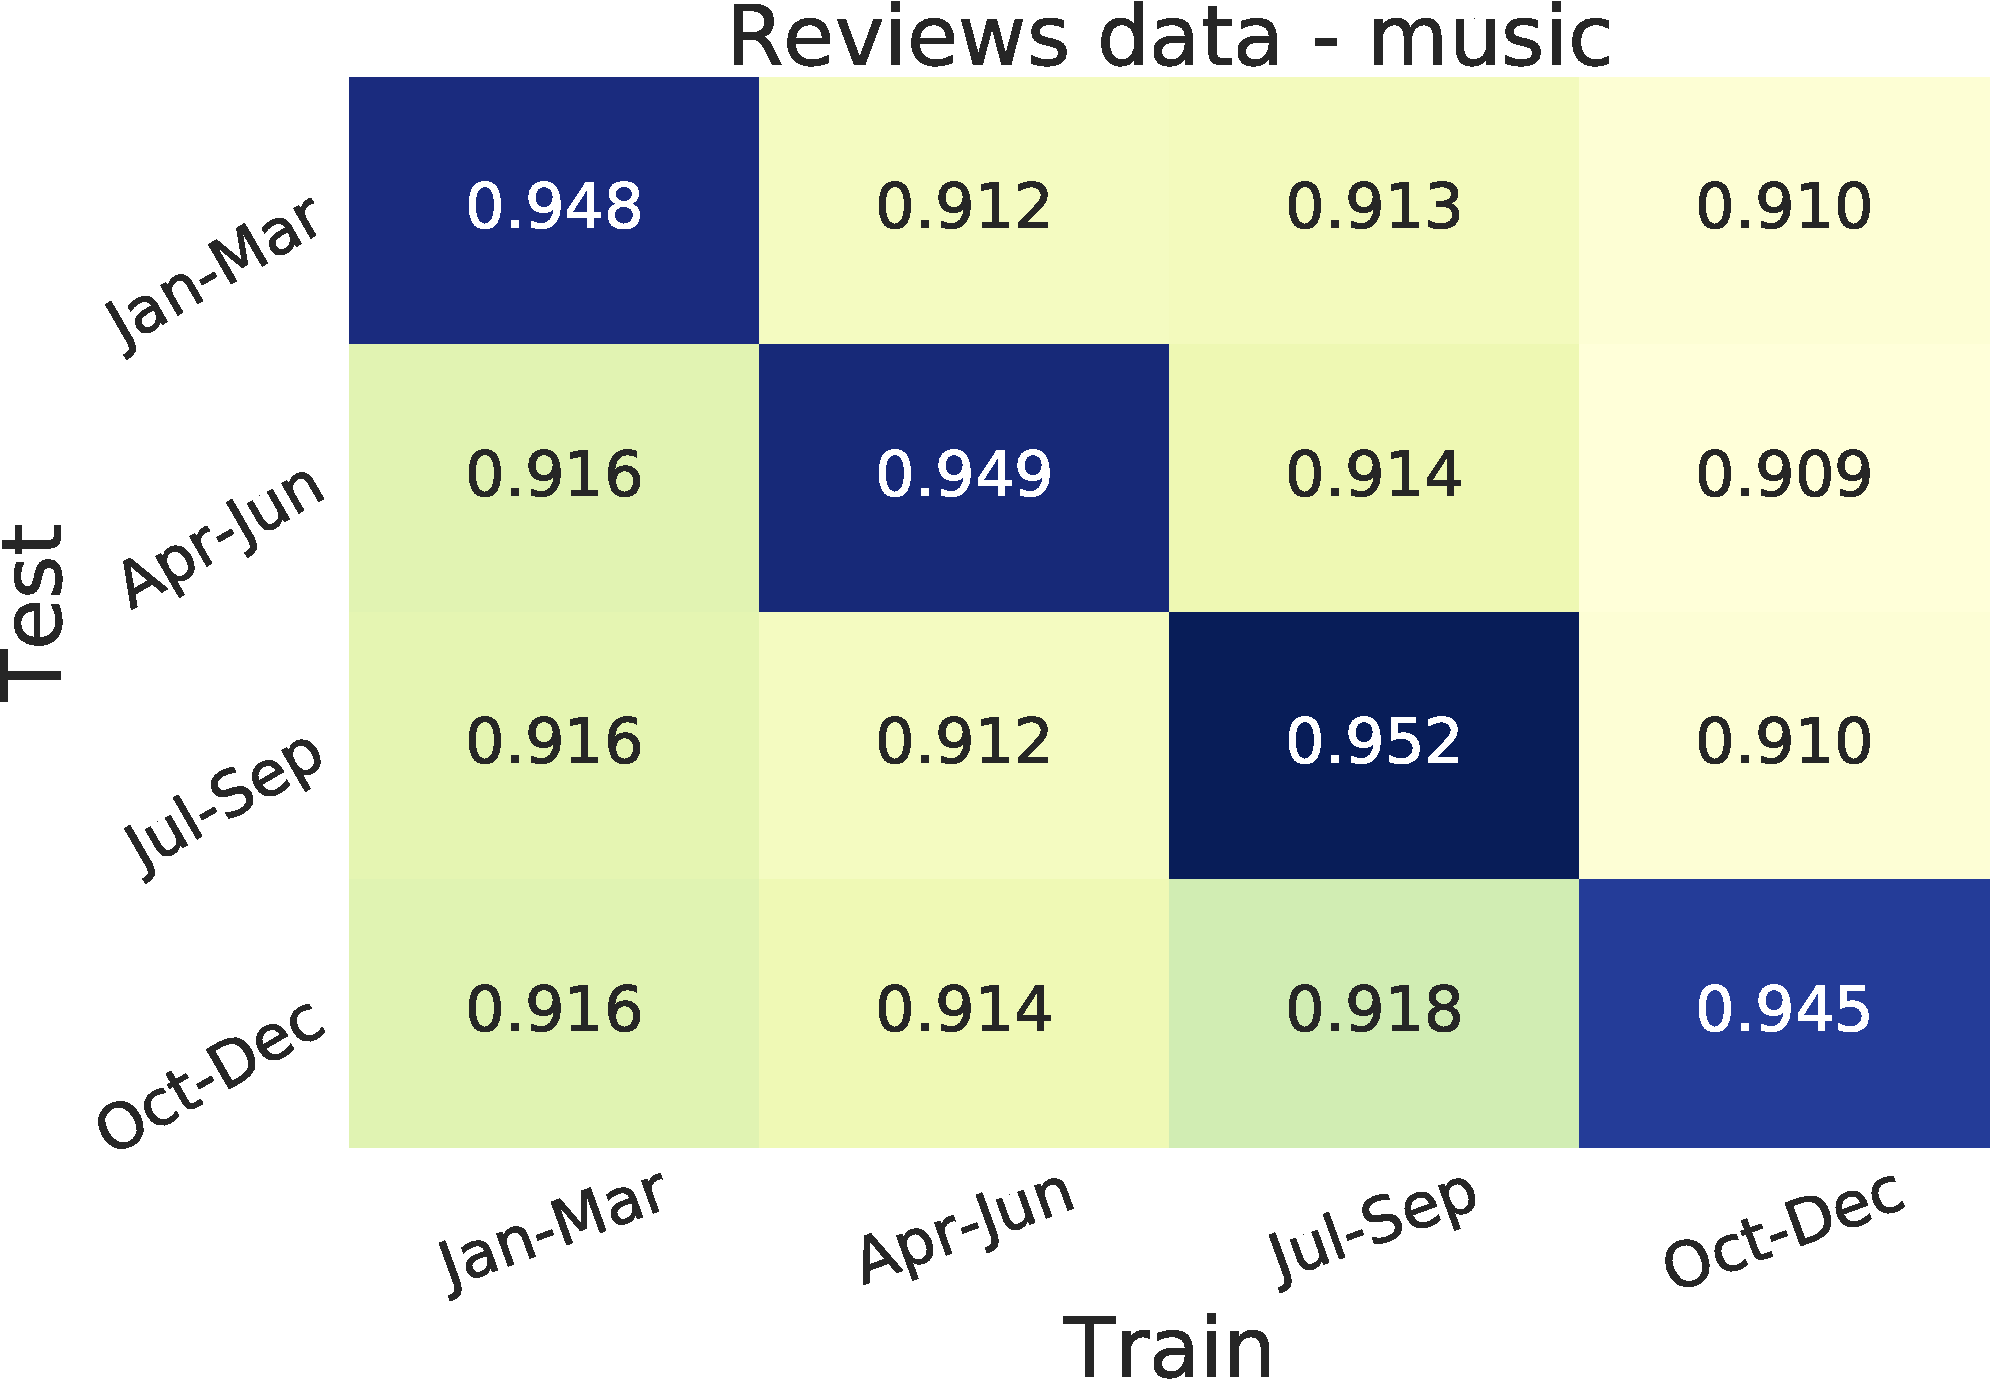
\includegraphics[width=0.244\textwidth]{images/chapter3/acl2018/month_amazon}
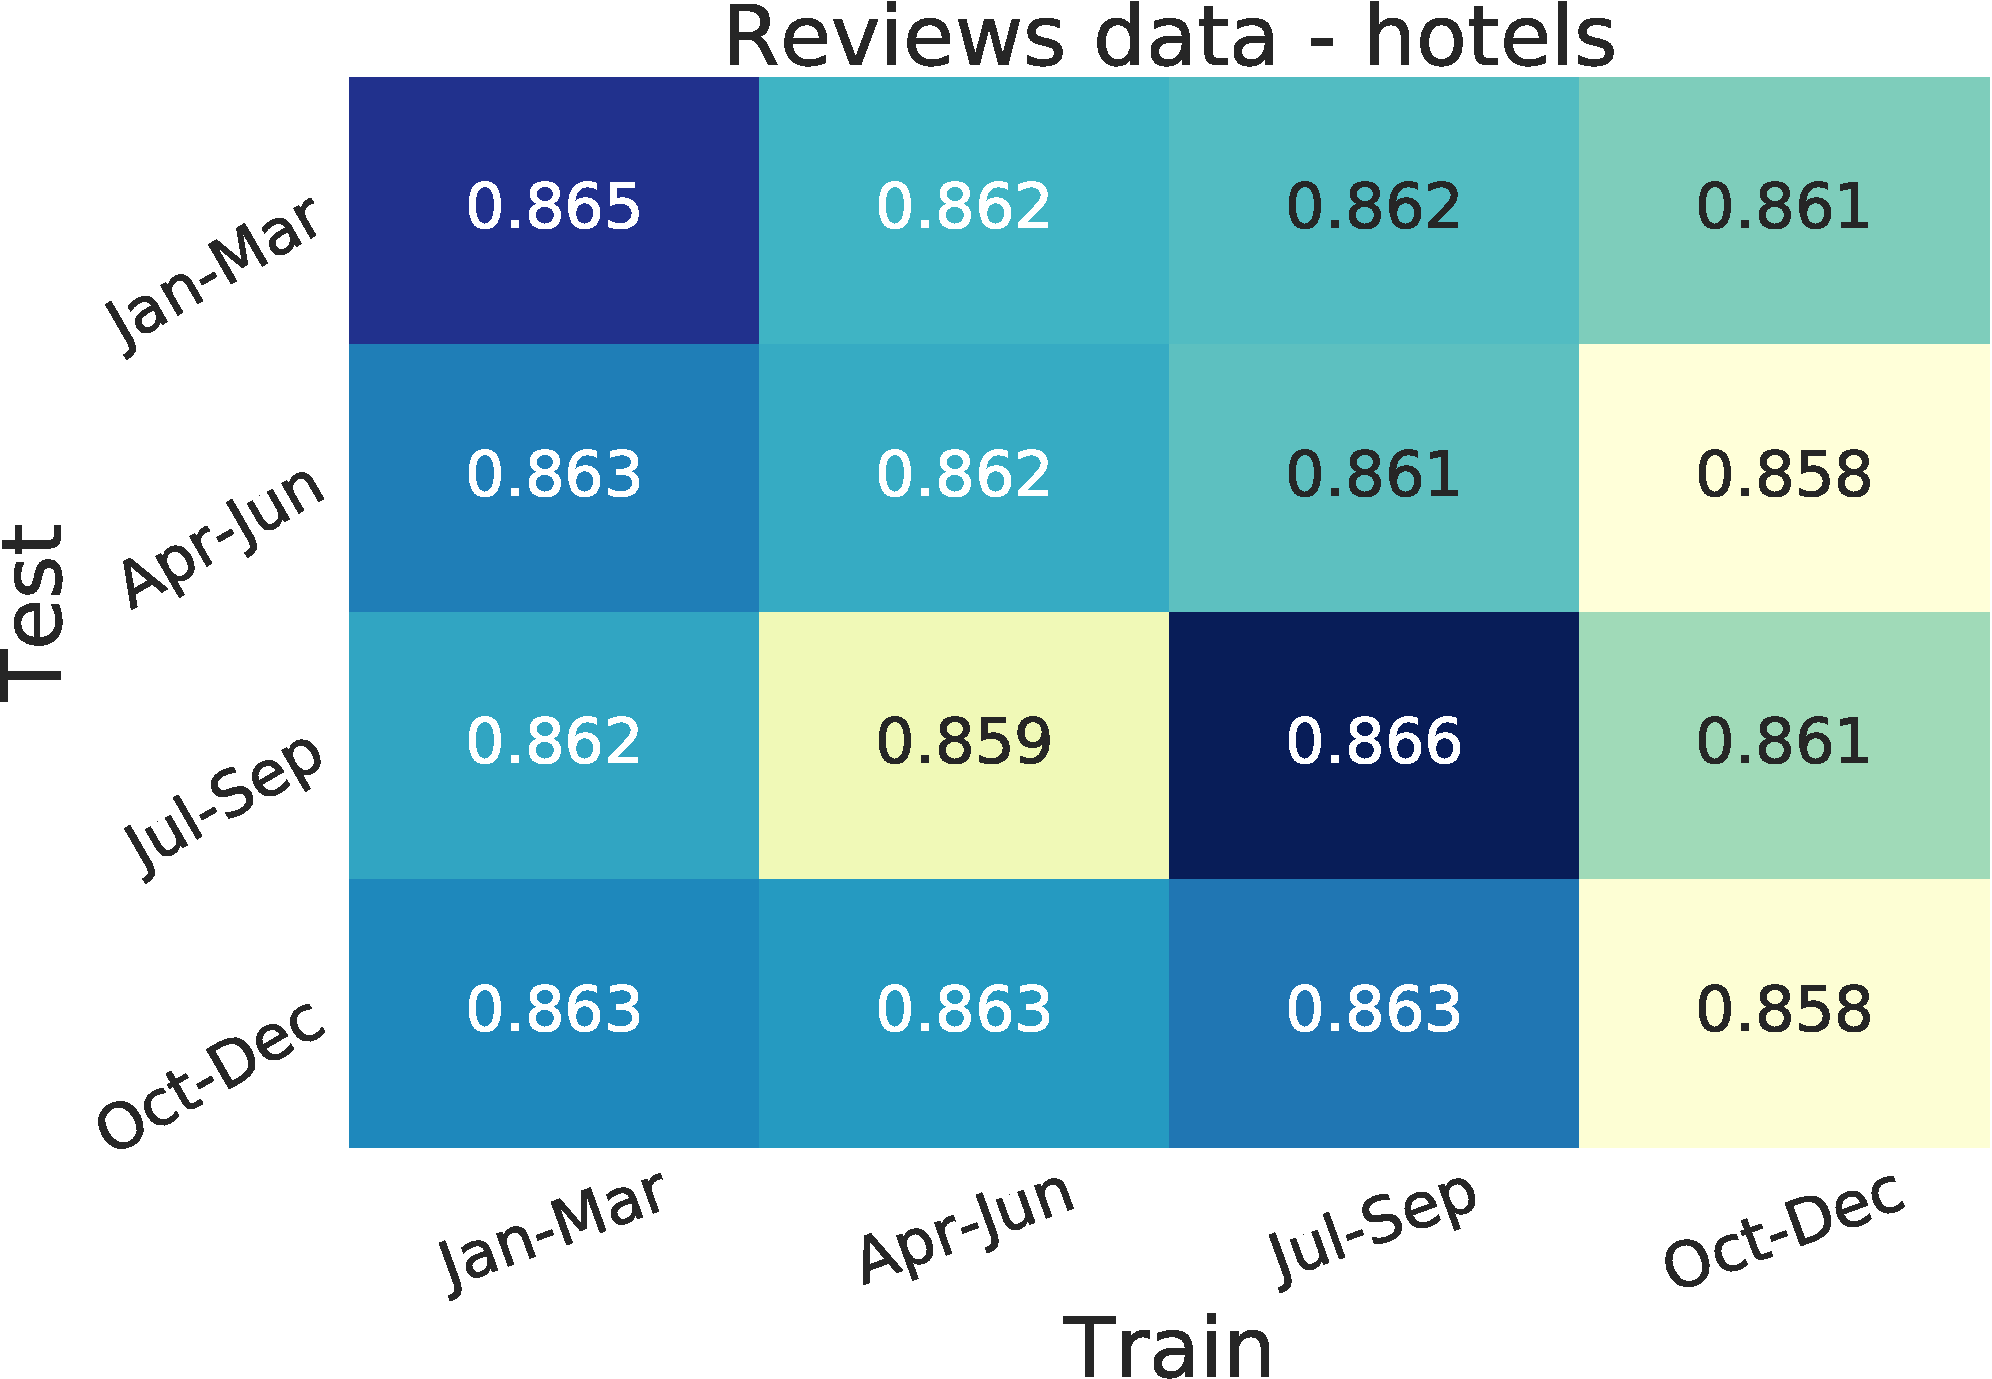
\includegraphics[width=0.244\textwidth]{images/chapter3/acl2018/month_hotel}
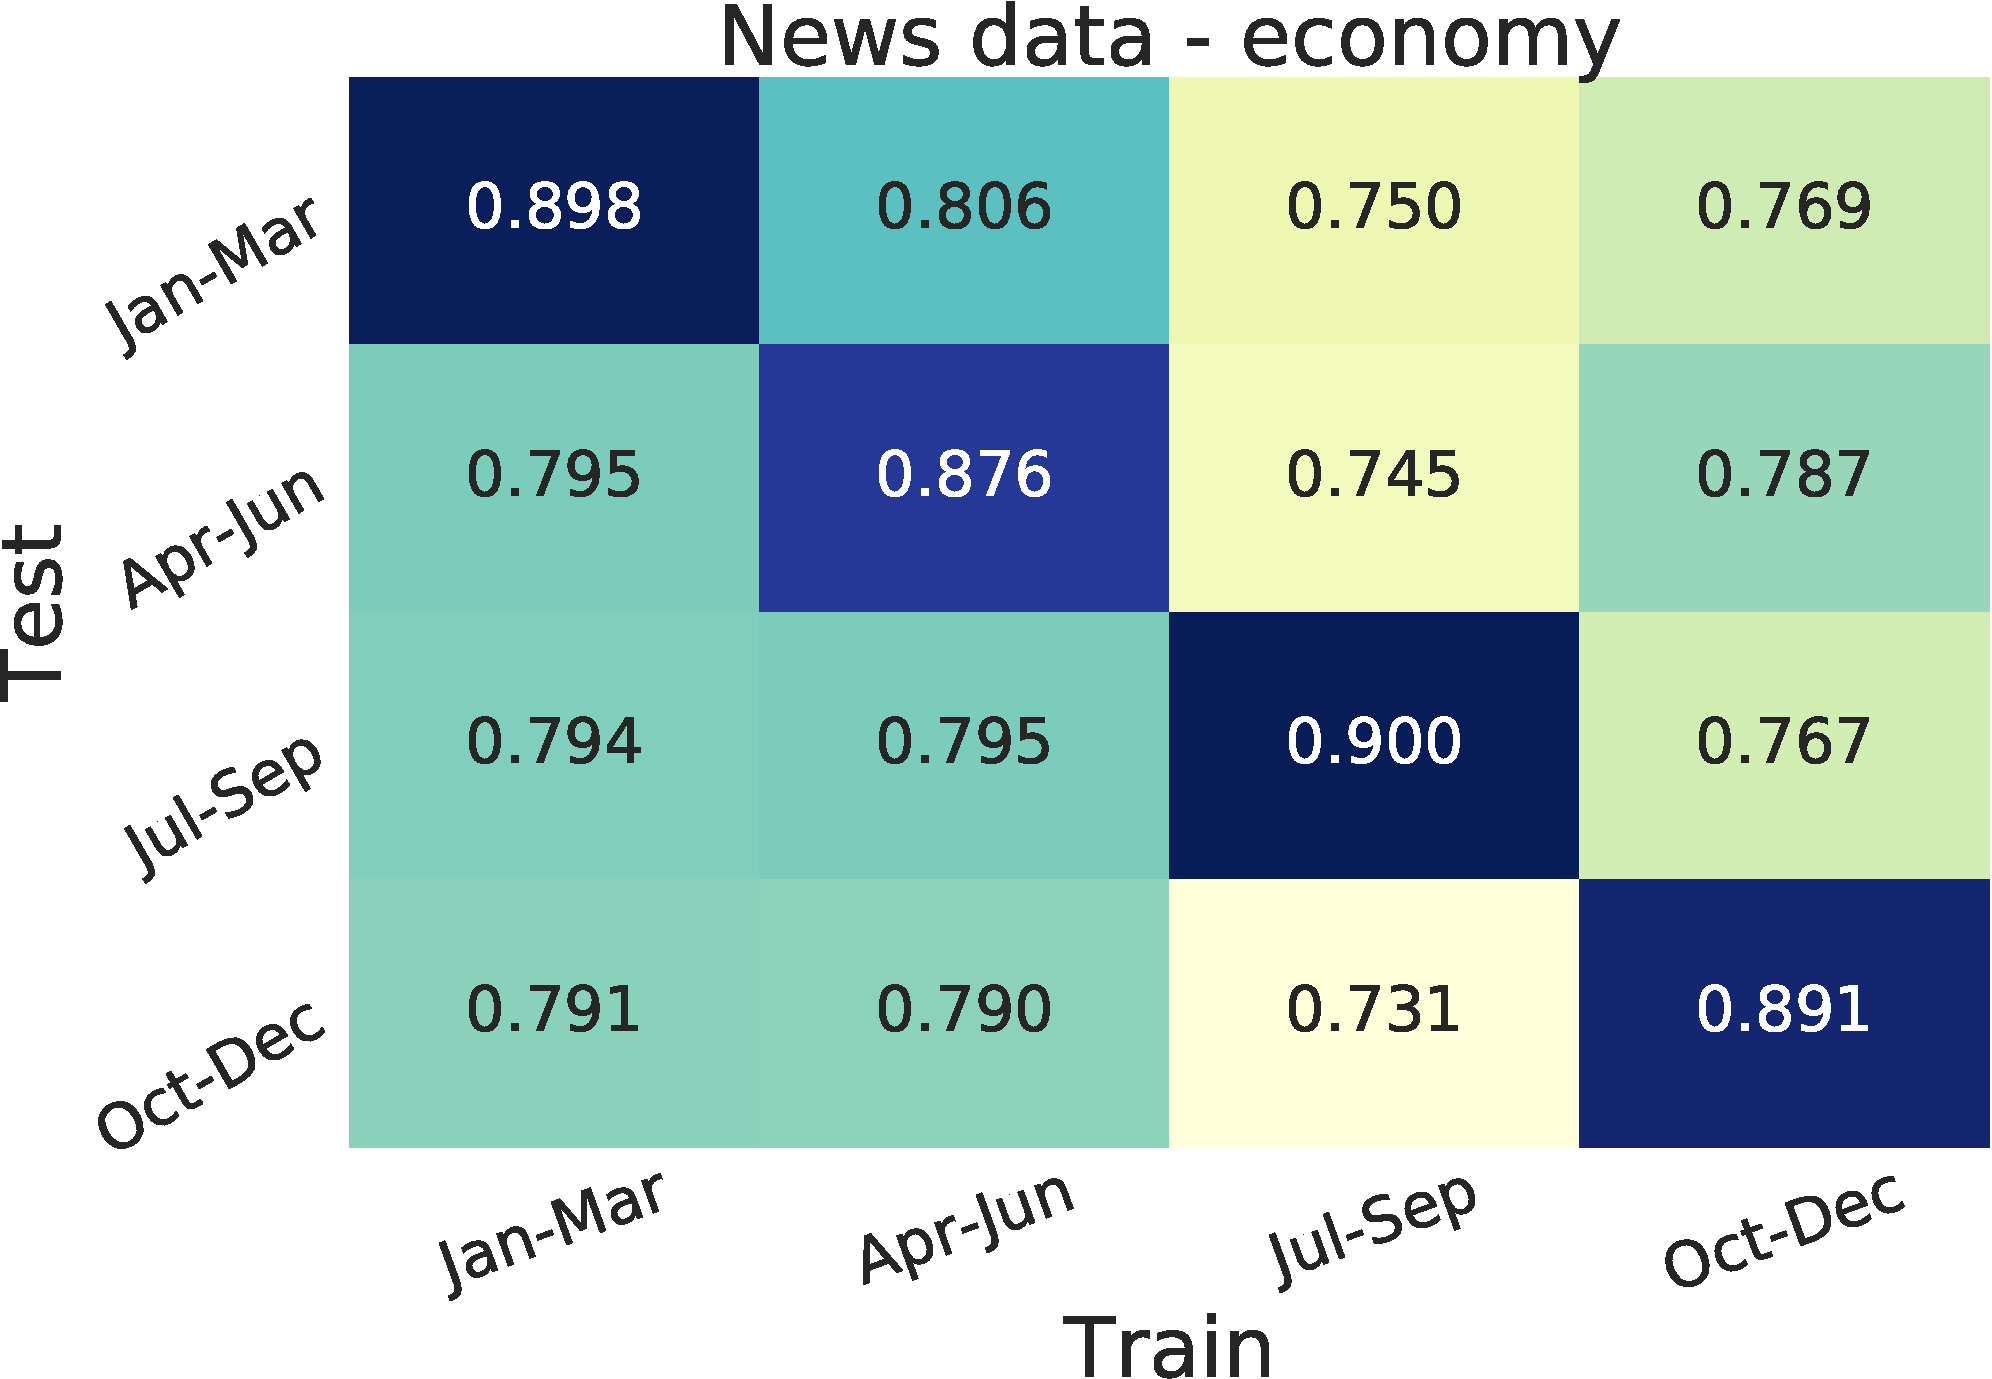
\includegraphics[width=0.244\textwidth]{images/chapter3/acl2018/month_economy}
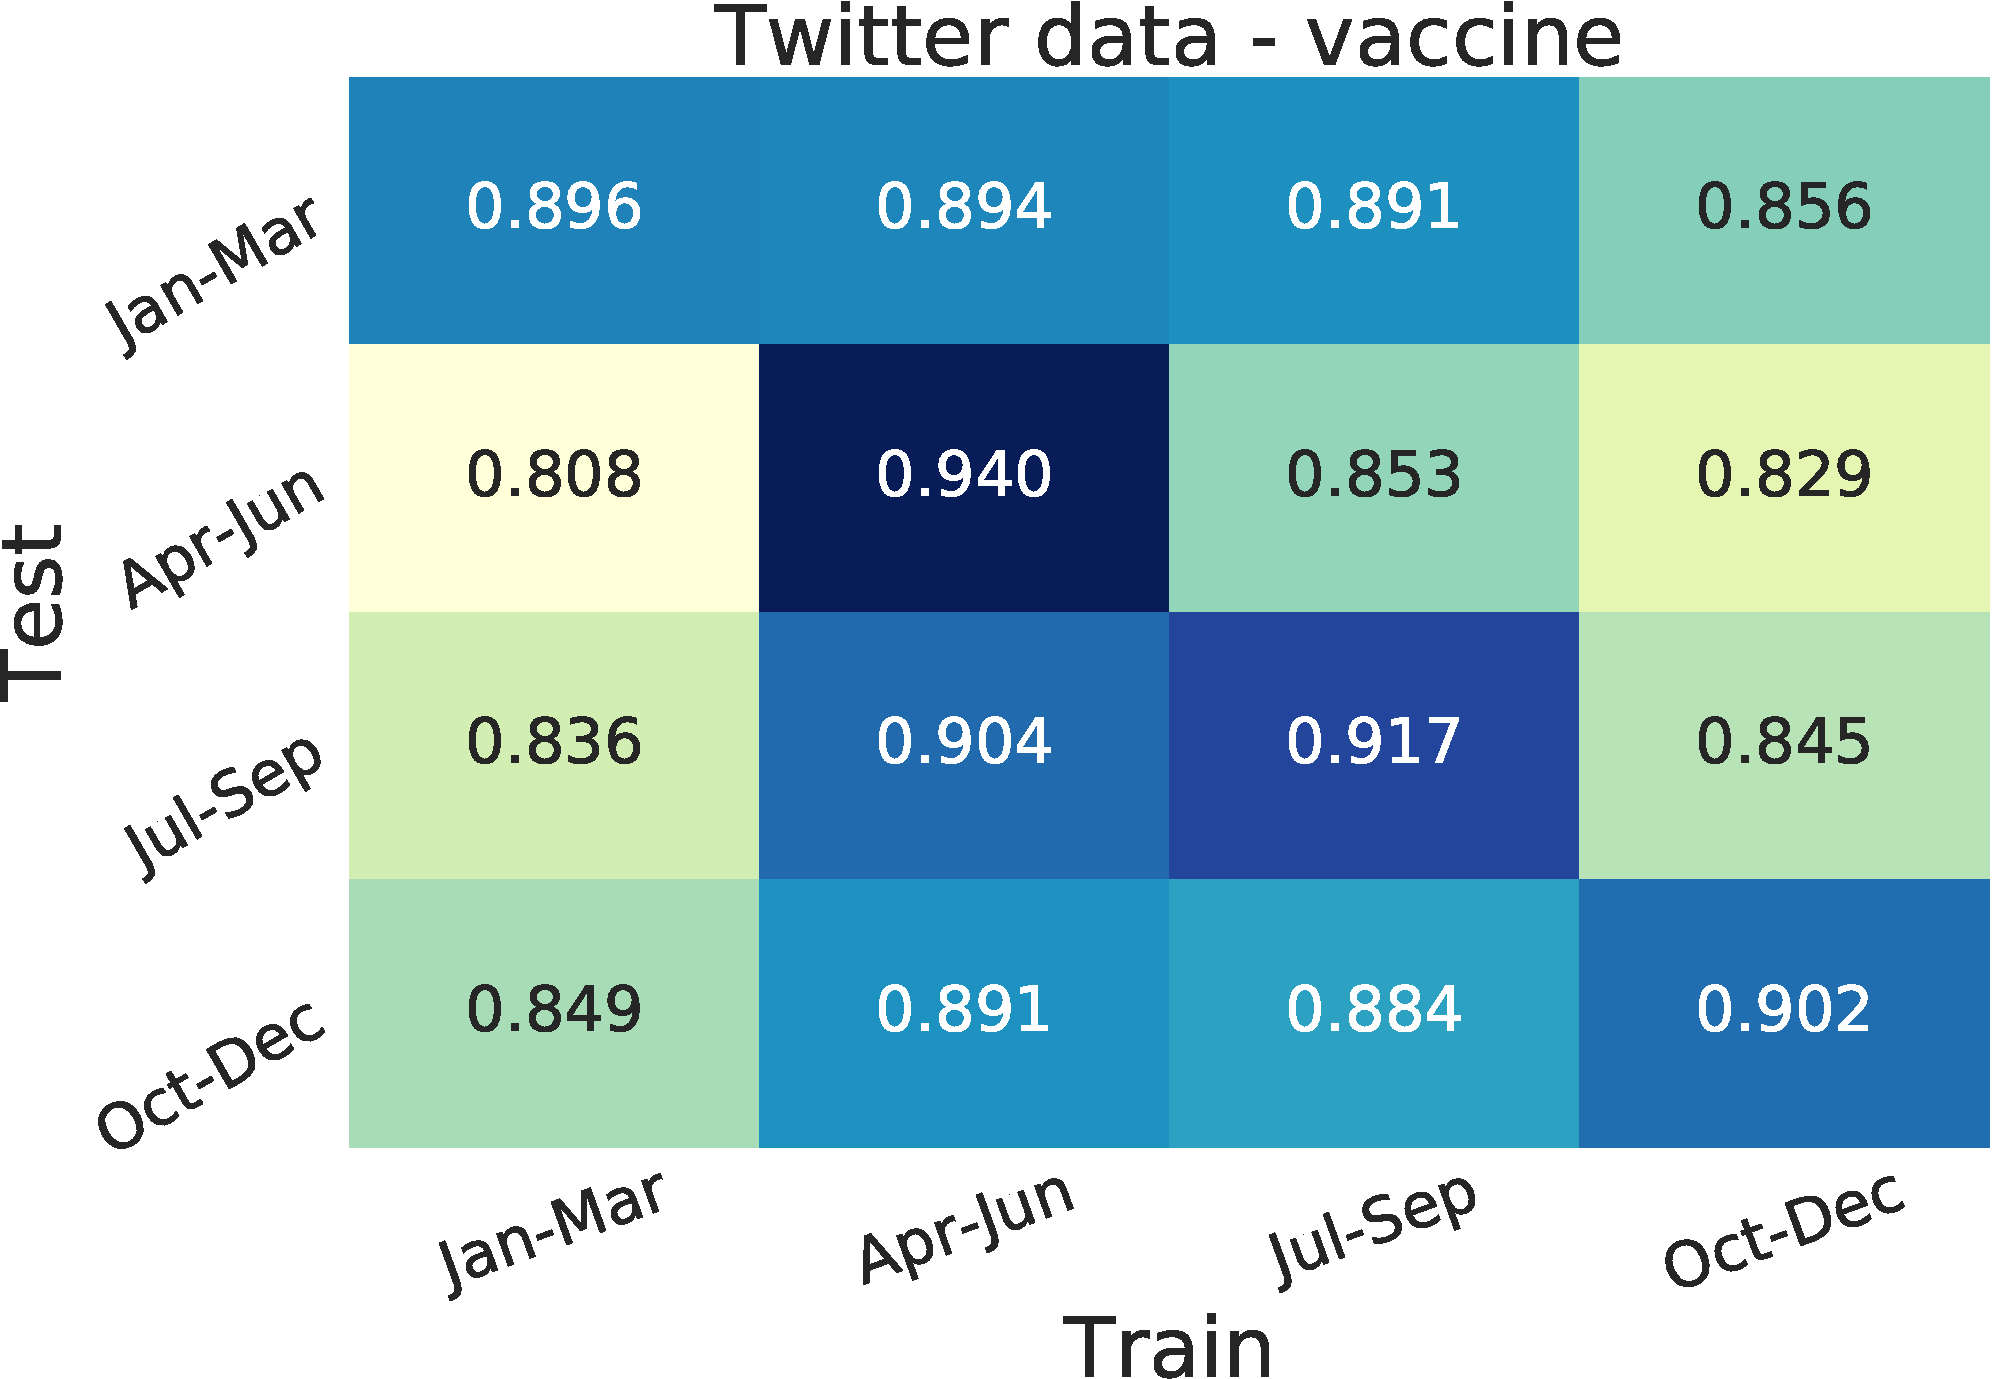
\includegraphics[width=0.244\textwidth]{images/chapter3/acl2018/month_vaccine} \\

\vspace{2ex}

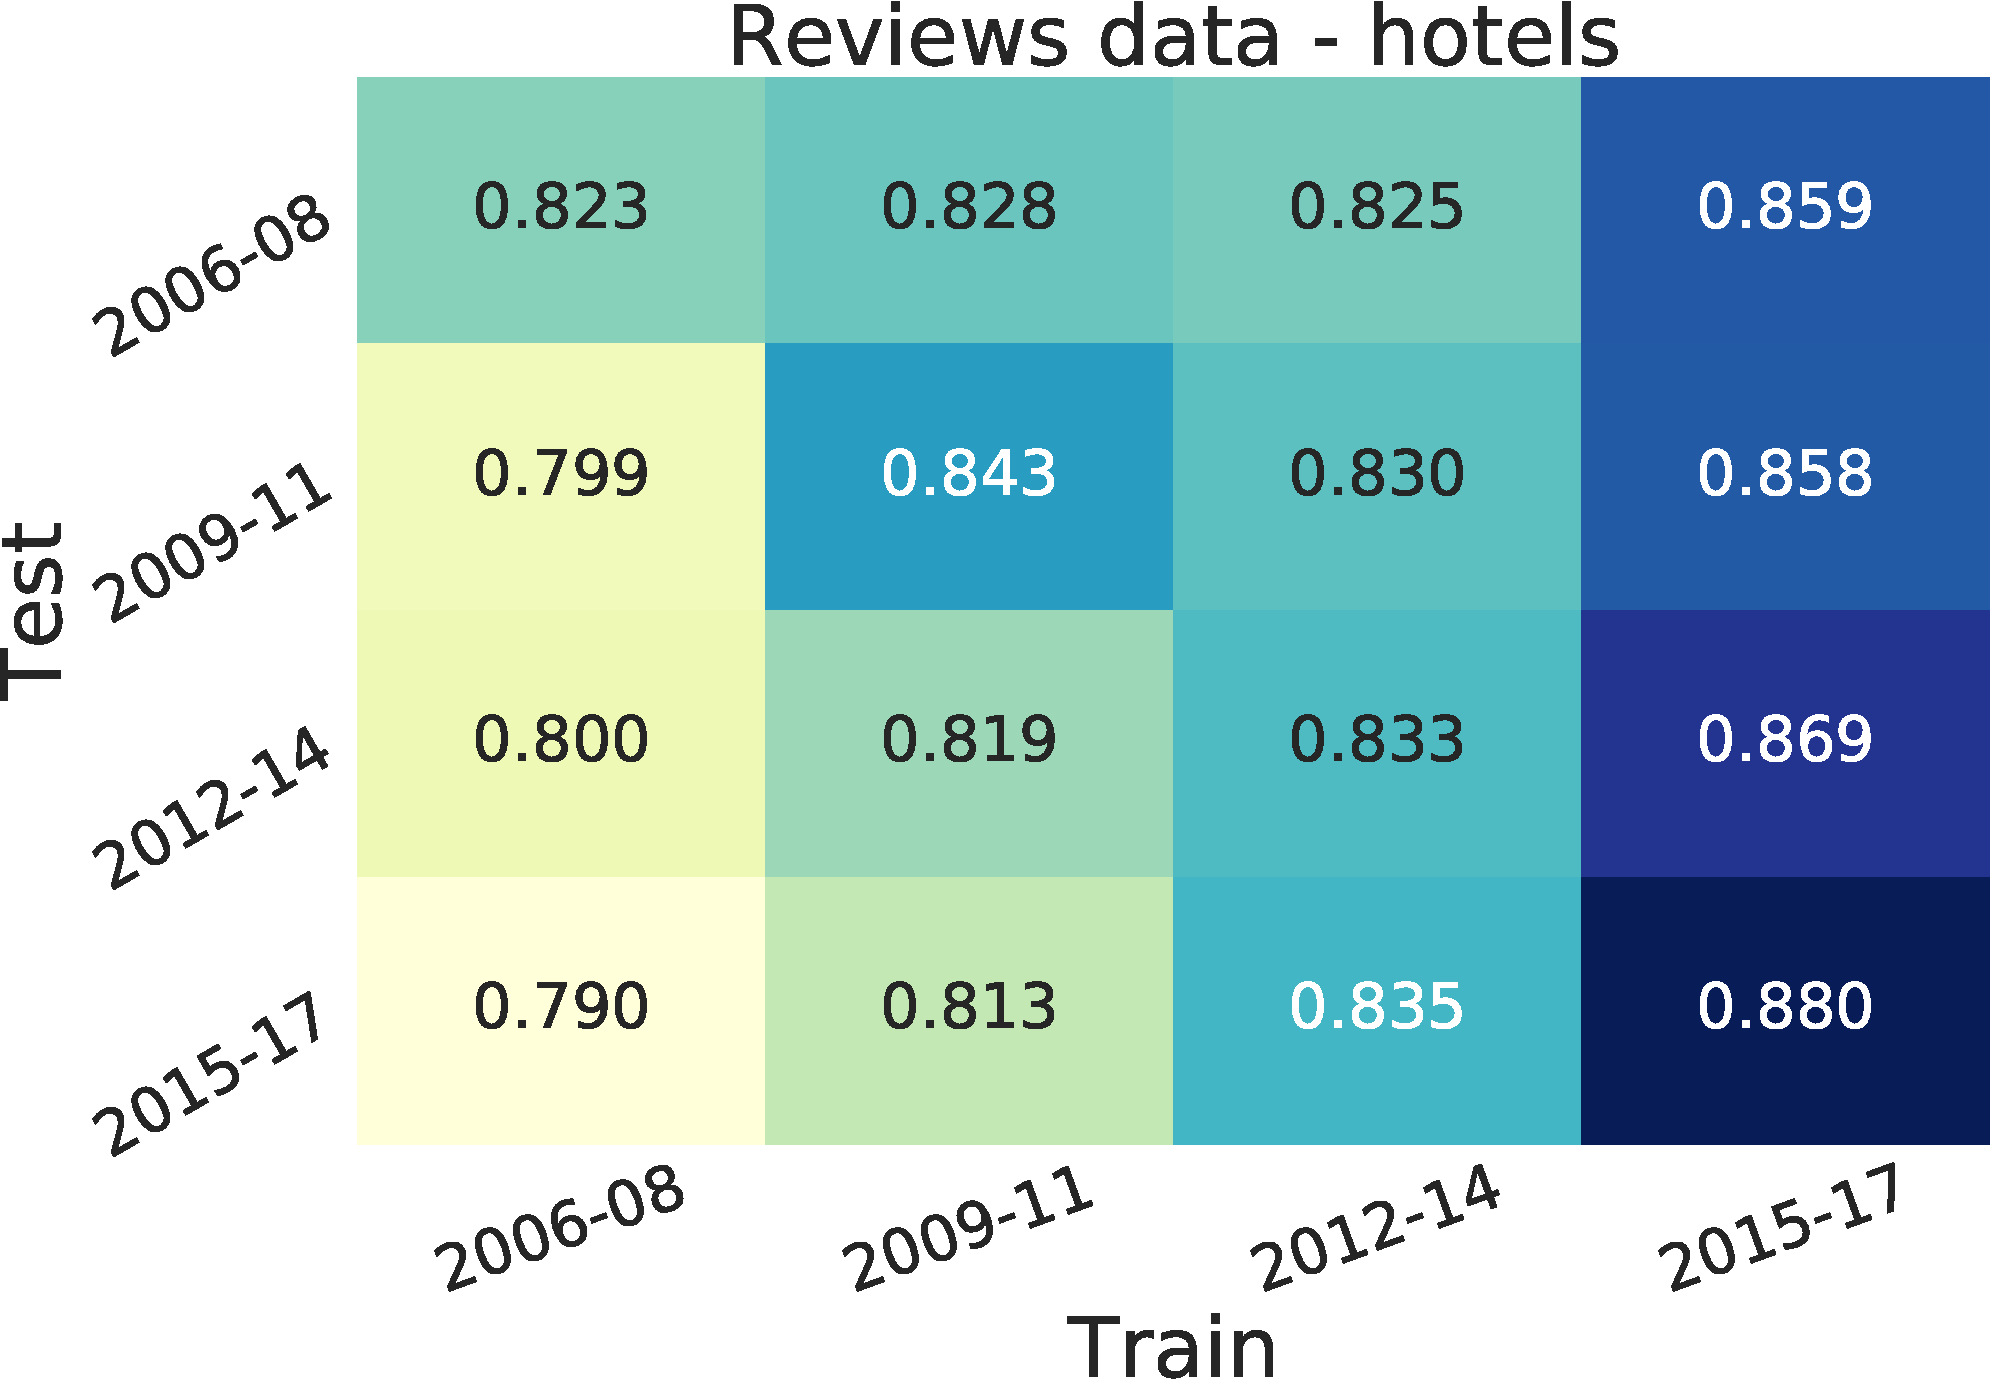
\includegraphics[width=0.244\textwidth]{images/chapter3/acl2018/year_hotel}
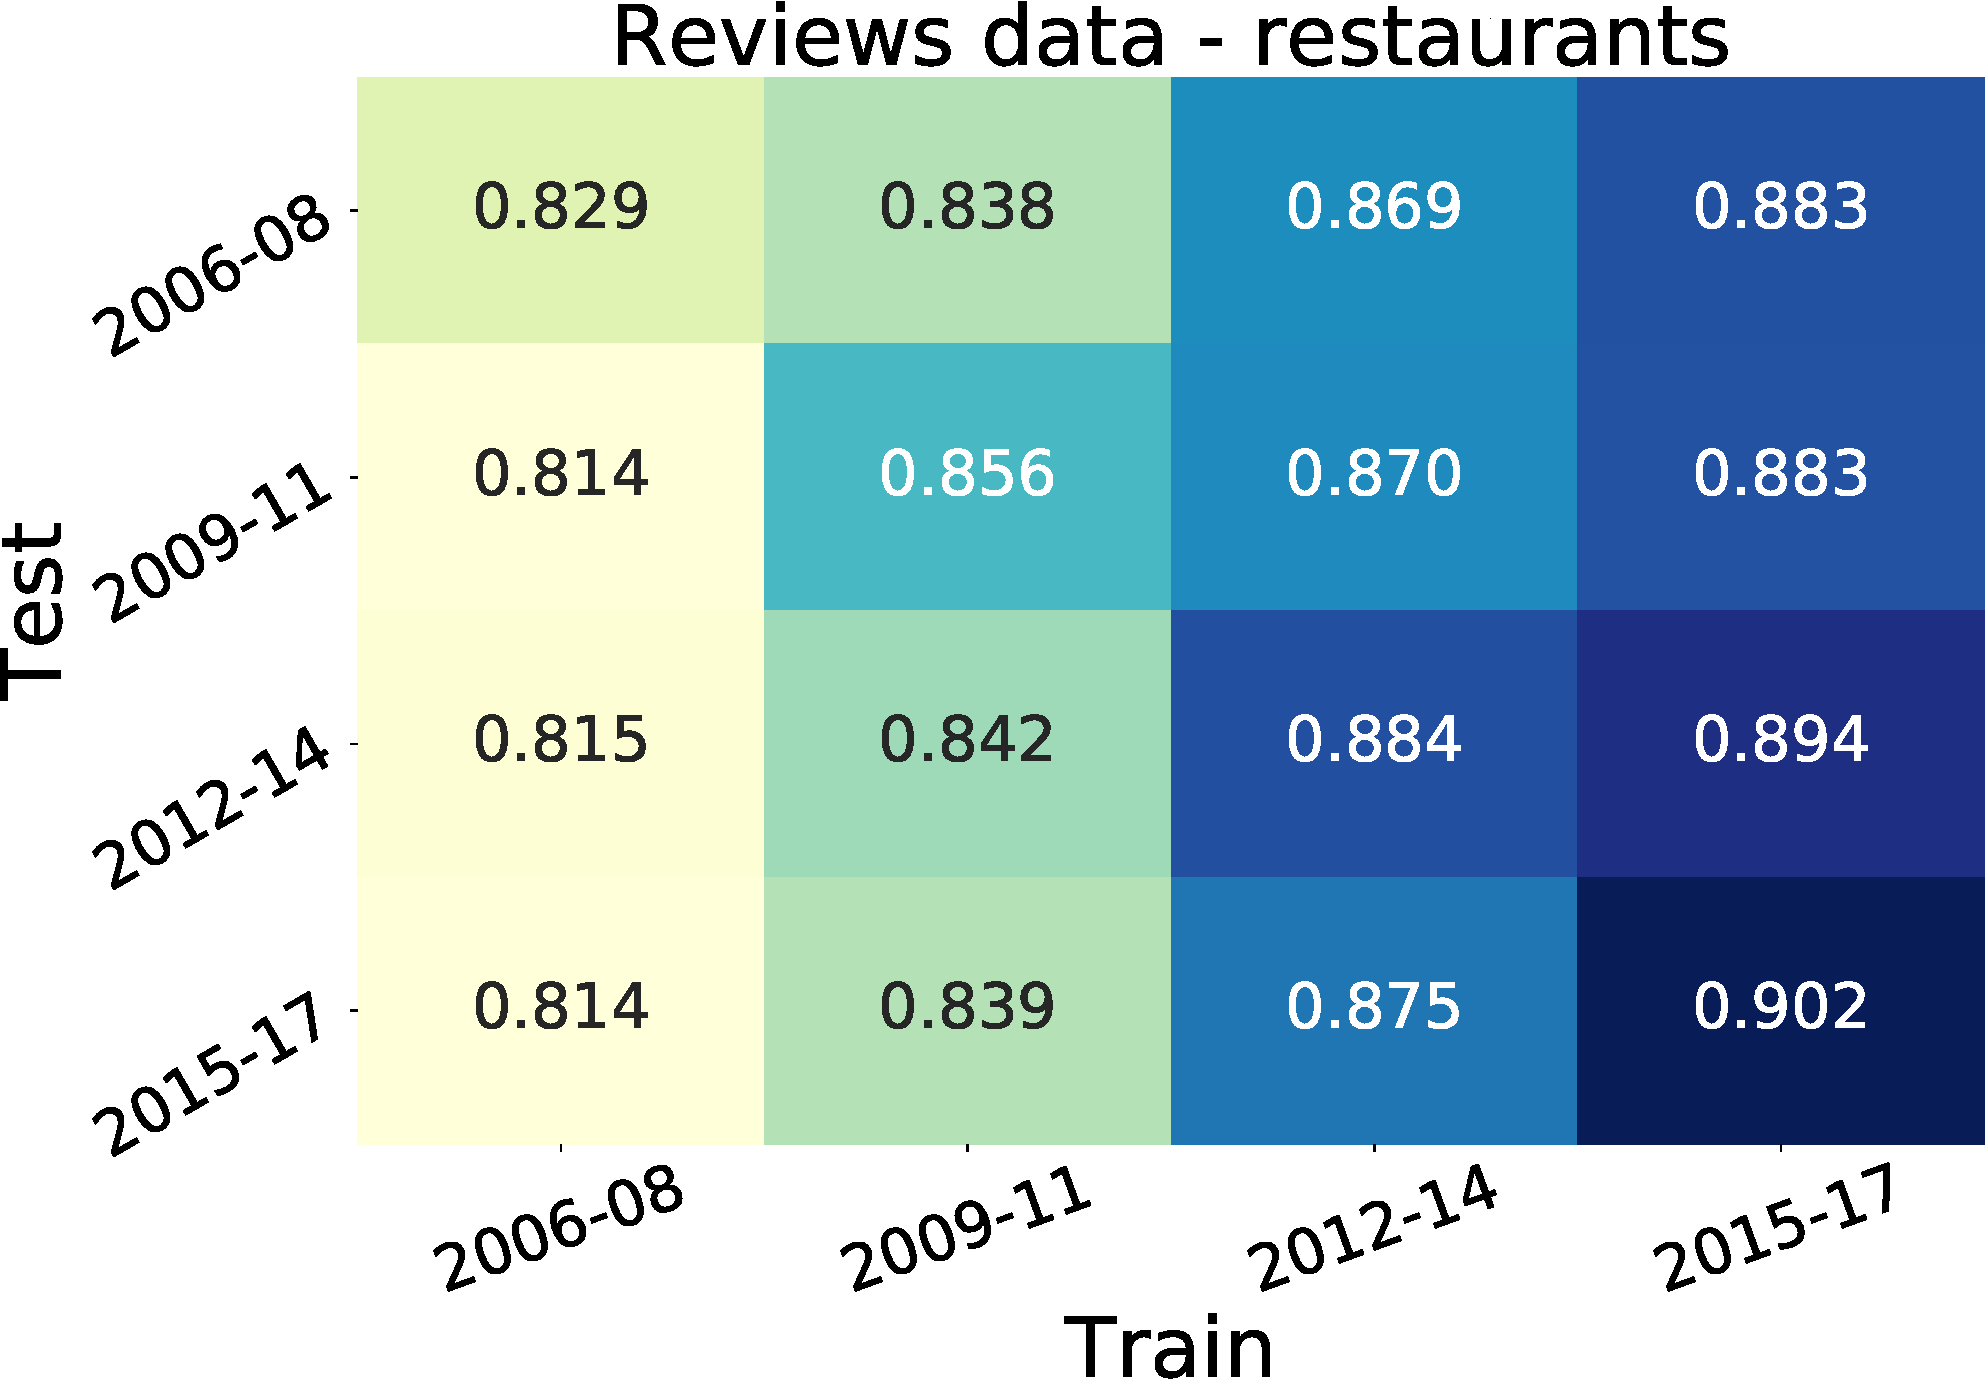
\includegraphics[width=0.244\textwidth]{images/chapter3/acl2018/year_rest}
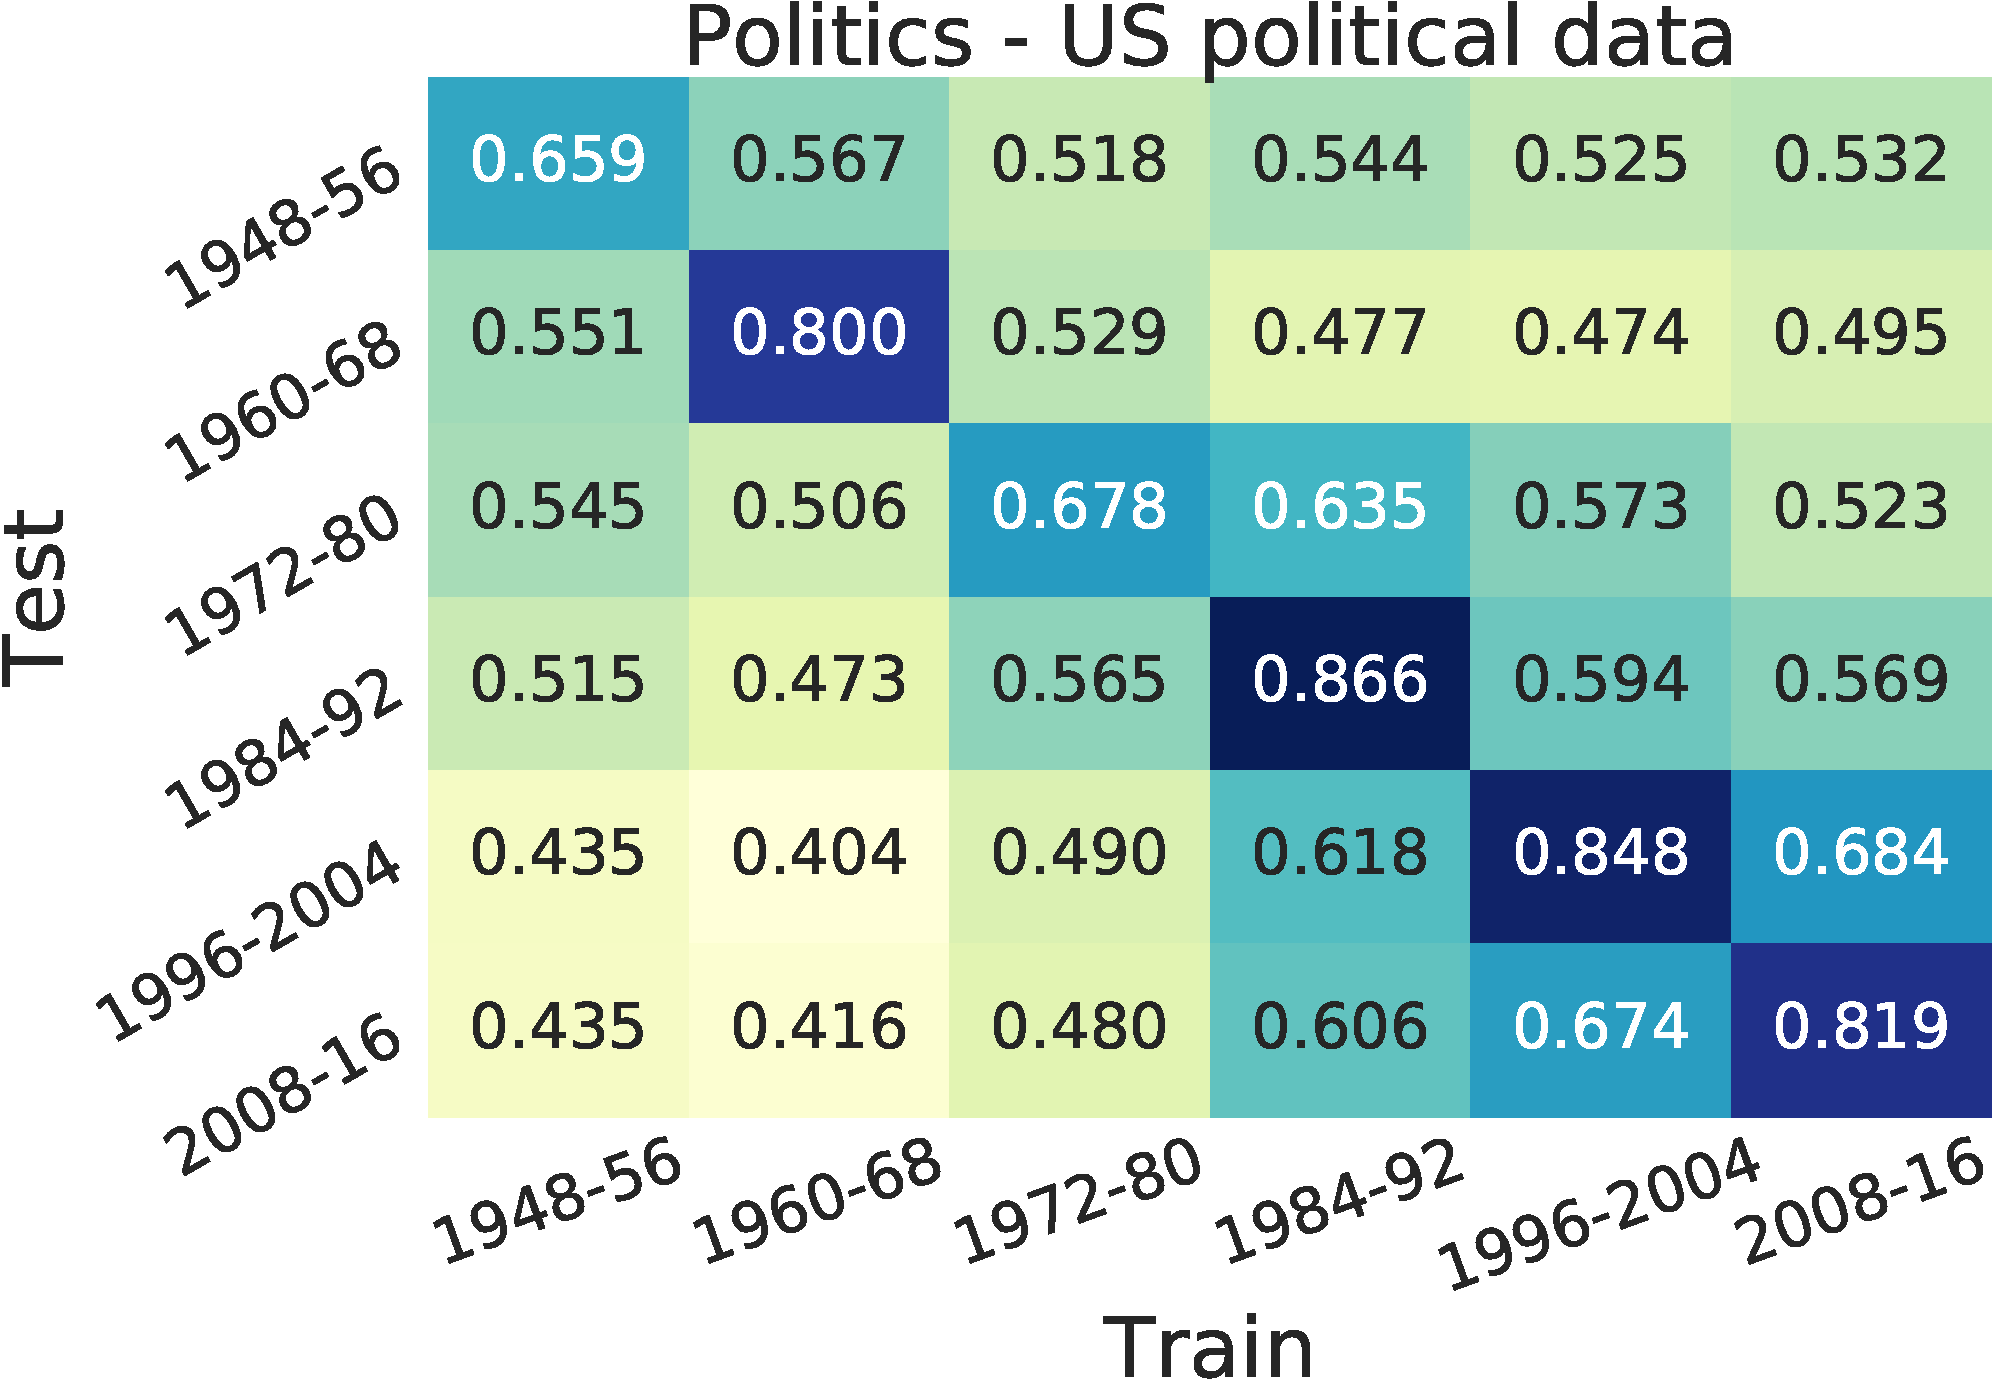
\includegraphics[width=0.244\textwidth]{images/chapter3/acl2018/year_parties}
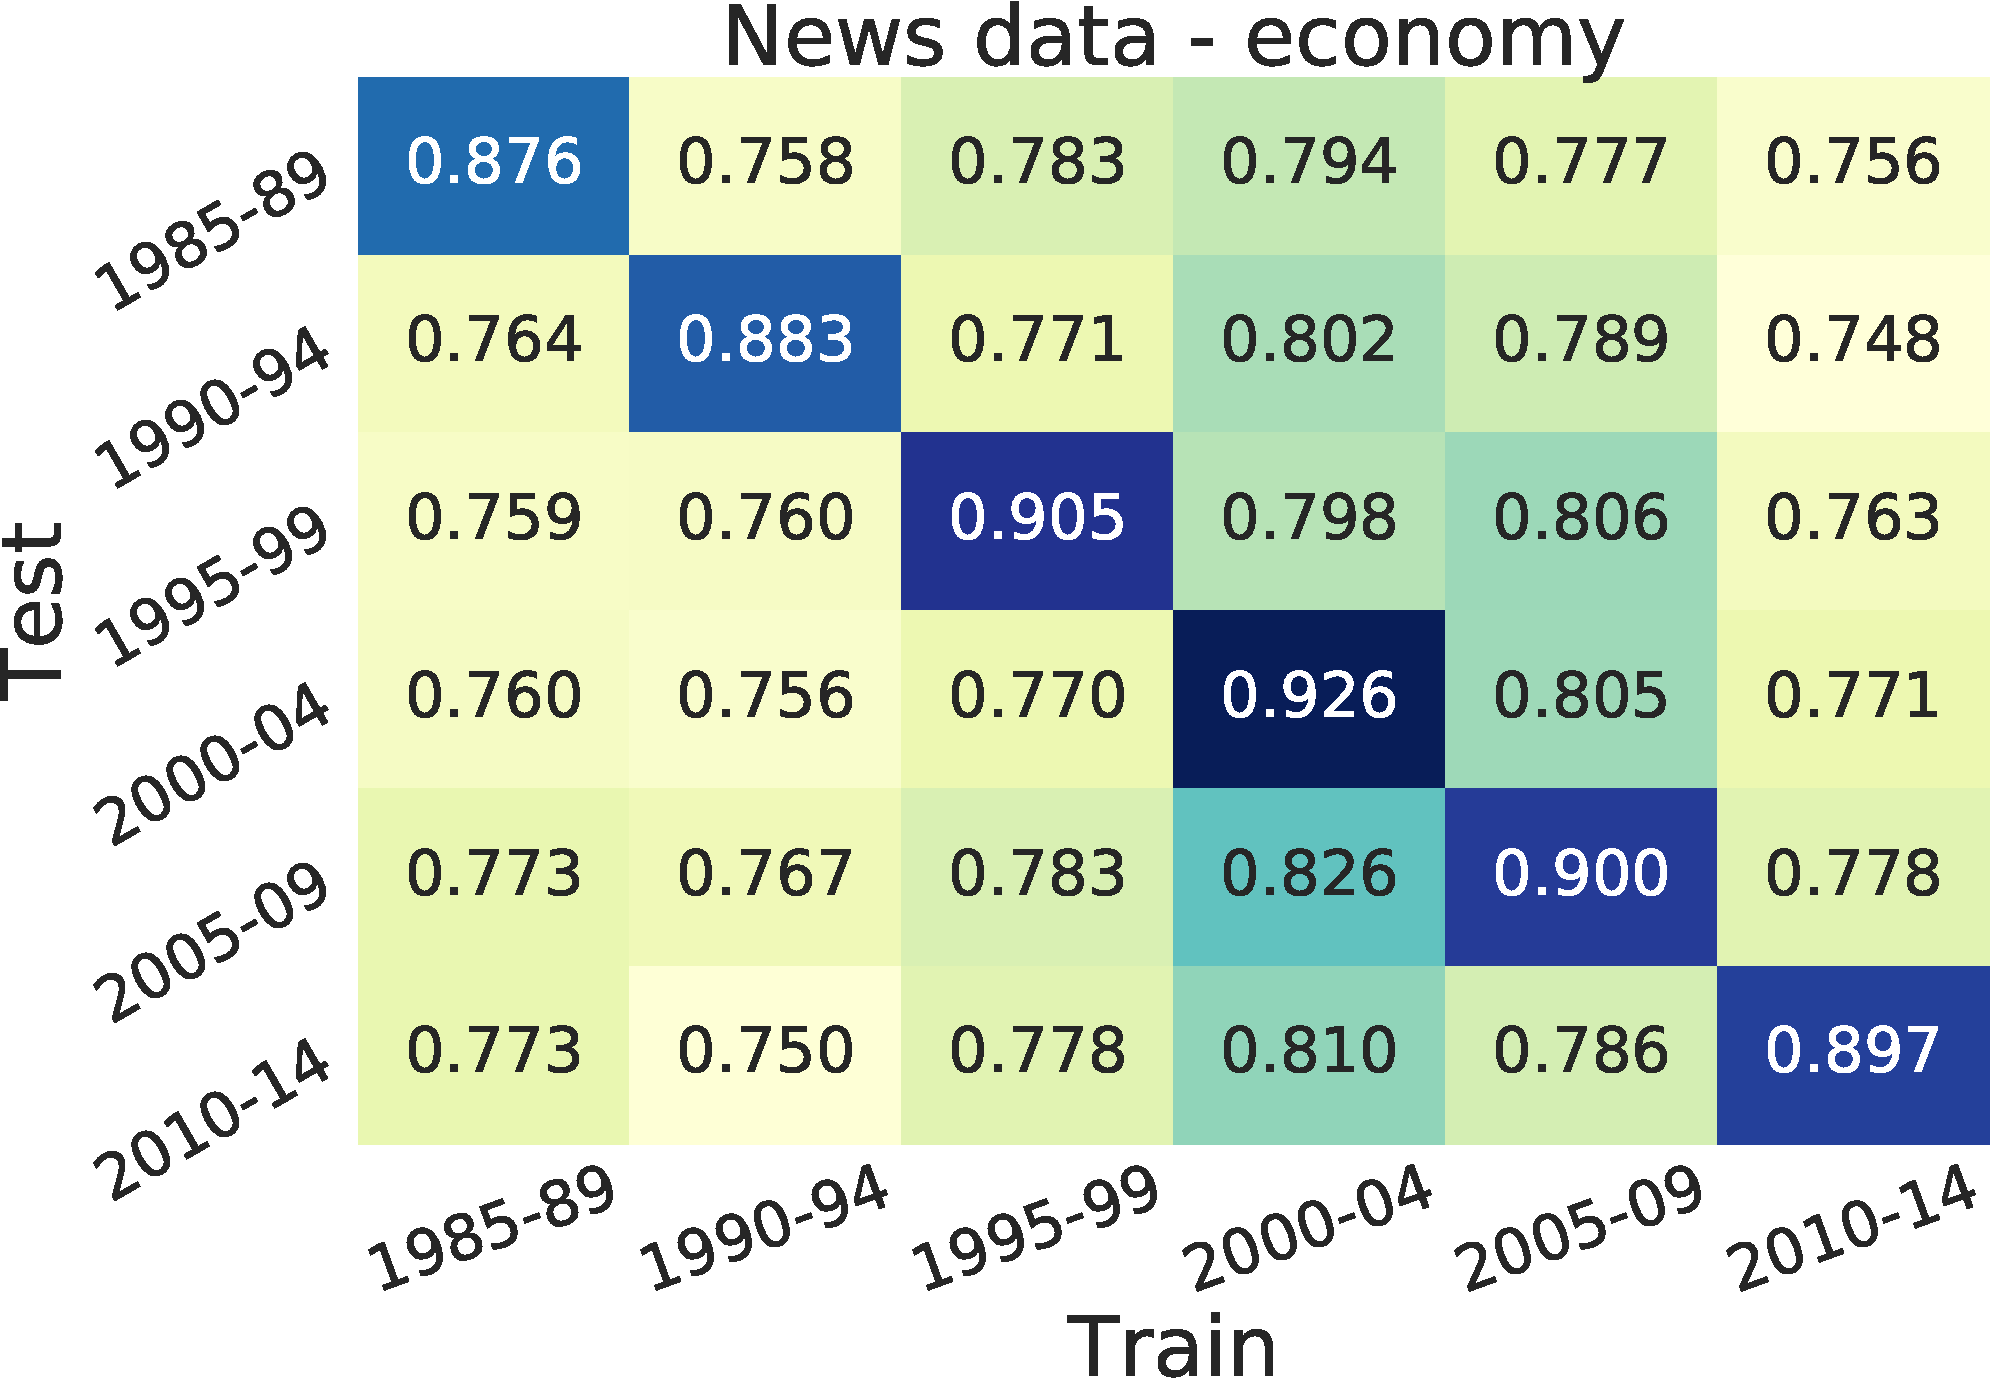
\includegraphics[width=0.244\textwidth]{images/chapter3/acl2018/year_economy}
\caption{\label{chap3:fig:time} Document classification performance when training and testing on different times of year (top) and different years (bottom). The datasets come from Amazon music reviews, Yelp hotel reviews, Economical news reports and Twitter. Darker indicate better classification performance.}
\end{figure*}

The Section \ref{chap3:subsec:wusage}, \ref{chap3:subsec:ctt_shift} and \ref{chap3:subsec:topic} show document features from word, context and topic have shifted overtime. In this section, we investigate how the shifts impact the performance of document classifiers.

We first conduct an analysis of how classifier performance depends on the time interval in which it is trained and applied.
For each corpus, we train the classifier on each time interval and test on each time interval.
To keep the same labeling format, reviews with neutral scores were removed.
We downsampled the training data within each time interval to match the number of documents in the smallest interval, so that differences in performance are not due to the size of the training data.

In all experiments, we train a classifier on a partition of 80\% of the documents in the time interval, and repeat this five times on different partitions, averaging the five F1 scores to produce the final estimate. When training and testing on the same interval, we test on the held-out 20\% of documents in that interval (standard cross-validation).
When testing on different time intervals, we test on all documents, since they are all held-out from the training interval; however, we still train on five subsets of 80\% of documents, so that the training data is identical across all experiments.

Figure~\ref{chap3:fig:time} can demonstrate that the temporal variations directly impact the performance of document classifiers: 
\begin{itemize}
    \item Classifiers perform best when applied to the same time interval they were trained, and performance diminishes when applied to other time intervals;
    \item Classifiers generally perform worse on farther time intervals than closer time intervals.
\end{itemize}

\subsection{Preprocessing}
We use NLTK~\cite{bird2004nltk} to tokenize the English corpora and the Jieba Python module~\cite{sun2012jieba} to segment the Chinese data. 
We discard reviews that had fewer than 10 tokens. 
For the Twitter data, we anonymize the data and replace usernames, hyperlinks and hashtags with ``USER'', ``URL'', ``HASHTAG'' respectively. 
All other text is lowercased.
For the four review datasets (Amazon, Dianping, Yelp restaurant and hotel) we encode the 5-point review score into three categories: reviews scores smaller than 3 were labeled as ``0'', larger than 3 are labeled as ``2'' and labeled as ``1'' if the score is 3. We binarize labels of the newspaper, political and Twitter data. 


\section{Feature Augmentation}
\label{chap3:sec:fa}

We now consider how to improve classifiers when working with datasets that span different time intervals.
We propose to treat this as a {\em domain adaptation} problem.
In domain adaptation, any partition of data that is expected to have a different distribution of features can be treated as a domain \cite{joshi2013s}.
Traditionally, domain adaptation is used to adapt models to a common task across rather different sets of data, e.g., a sentiment classifier for different types of products \cite{blitzer2007biographies}.
Recent work has also applied domain adaptation to adjust for potentially more subtle differences in data, such as adapting for differences in demographics of authors \cite{volkova2013exploring, lynn2017human}.
We follow the same approach, treating time intervals as domains.

In our experiments, we use the feature augmentation approach of \cite{daume2007frustratingly} to perform domain adaptation. Each feature is duplicated to have a specific version of the feature for every domain, as well as a domain-independent version of the feature. In each instance, the domain-independent feature and the domain-specific feature for that instance's domain have the same feature value, while the value is zeroed out for the domain-specific features for the other domains. This is equivalent to a model where the feature weights are domain-specific but share a Gaussian prior across domains \cite{finkel2009hierarchical}.
This approach is widely used due to its simplicity, and derivatives of this approach have been used in similar work (e.g., \cite{lynn2017human}).
Following~\cite{finkel2009hierarchical}, we separately adjust the regularization strength for the domain-independent feature weights and the domain-specific feature weights.

\subsection{Experiments}

In this section, we conduct experiments on Amazon, Yelp, Twitter, Political and Economy datasets with both seasonal and non-seasonal spans. 
For consistency, we experiment the review datasets with binary labels by discarding documents with the neutral labels.

\subsubsection{Seasonal Adaptation}

\begin{table}[htp]
\centering
\begin{tabular}{|l|l|l|}
\hline
\bf Data (Seasonal) & \bf Baseline & \bf Adaptation \\
\hline
Amazon (reviews) & .901 & \bf .919 \\
Yelp-hotel (reviews) & .867 & \bf .881 \\
Yelp-rest (reviews) & .874 & \bf .898  \\
Economy (news) & .782 & .782  \\
Twitter (vaccines) & \bf .881 & .880  \\
\hline
\end{tabular}
\caption{\label{chap3:tab:results_seasonal} F1-weighted scores when treating each seasonal time interval as a domain and applying domain adaptation compared to using no adaptation.}
\end{table}

We first examine classification performance on the datasets when grouping the seasonal time intervals (January-March, April-June, July-August, September-December) as domains and applying the feature augmentation approach for domain adaptation. 
As a baseline comparison, we apply the same classifier, but without domain adaptation.

Results are shown in Table~\ref{chap3:tab:results_seasonal}.
We see that applying domain adaptation provides a small boost in three of the datasets and has no effect on two of the datasets.
If this pattern holds in other corpora, then this suggests that it does not hurt performance to apply domain adaptation across different times of a year, and in some cases can lead to a small performance boost.

\subsubsection{Non-seasonal Adaptation}
\label{subsec:nonseasonal}

\begin{table*}[htp]
\centering
\begin{tabular}{|l|l|l|l|}
\hline
\bf Data (Non-seasonal) & \bf Baseline & \bf Adaptation & \bf Adapt.+seasons \\
\hline
Amazon (reviews) & .895 & \bf .924 & .910 \\
Yelp-hotel (reviews) & .886 & .892 & \bf .920 \\
Yelp-rest (reviews) & .831 & .879 & \bf .889   \\
Economy (news) & .763 & .780 & \bf .859 \\
Politics (platforms) & .661 & \bf .665 & n/a \\
Twitter (vaccines) & .910 & .903 & \bf .920 \\
\hline
\end{tabular}
\caption{\label{chap3:tab:results_nonseasonal_future} F1 scores when testing on the final time interval after training on all previous intervals.}
\end{table*}

We now consider the non-seasonal time intervals (spans of years). 
In particular, we consider the scenario when one wants to apply a classifier trained on older data to {\em future} data.
This requires a modification to the domain adaptation approach, because future data includes domains that did not exist in the training data, and thus we cannot learn domain-specific feature weights.
To solve this, we train in the usual way, but when testing on future data, we only include the domain-independent features.
The intuition is that the domain-independent parameters should be applicable to all domains, and so using only these features should lead to better generalizability to new domains.
We test this hypothesis by training the classifiers on all but the last time interval and testing on the final interval.
For hyperparameter tuning, we used the final time interval of the training data (i.e., the penultimate interval) as the validation set. The intuition is that the penultimate interval is the closest to the test data and thus is expected to be most similar to it.

Results are shown in the first three columns of Table~\ref{chap3:tab:results_nonseasonal_future}.
We see that this approach leads to a small performance boost in all cases except the Twitter dataset. 
This means that this simple feature augmentation approach has the potential to make classifiers more robust to future changes in data.

How to apply the feature augmentation technique to unseen domains is not well understood.
By removing the domain-specific features, as we did here, the prediction model has changed, and so its behavior may be hard to predict.
Nonetheless, this appears to be a successful approach.

\subsubsection{Dual Adaptation}

We also experimented with including the seasonal features when performing non-seasonal adaptation.
In this setting, we train the models with two domain-specific features in addition to the domain-independent features: one for the season and one for the non-seasonal interval. 
As above, we remove the non-seasonal features at test time; however, we retain the season-specific features in addition to the domain-independent features, as they can be reused in future years.

The results of this approach are shown in the last column of Table~\ref{chap3:tab:results_nonseasonal_future}.
We find that combining seasonal and non-seasonal features leads to an additional performance gain in most cases.


\section{Diachronic Word Embeddings}
\label{chap3:sec:dwe}

Standard word embeddings ignore temporal language variations in the data.
\textit{Diachronic} word embeddings~\cite{kulkarni2015statistically} 
encode temporality into word embeddings to obtain dynamic representations of words. 
These types of embeddings have been effective in capturing and learning the language usage and semantic shift over time~\cite{kim2014temporal, kulkarni2015statistically, hamilton2016diachronic, bamler2017dynamic, szymanski2017temporal, rudolph2018dynamic, rosenfeld2018deep, yao2018dynamic}. 

To the best of our knowledge, diachronic word embeddings have not been studied in the context of document classification. 
Since our preliminary analyses in the previous section (Section~\ref{chap3:sec:data}) showed that the top features for document classification vary over time, and the contexts used to train those word embeddings also vary over time, 
it would make sense to use word representations that can vary over time.
In this section, we present a new, simple-to-implement method for constructing diachronic embeddings, and then further analyze temporal shifts in corpora using these embeddings.

\subsection{Concatenative Training Approach}

Methods to obtain diachronic word embeddings fall into three main directions: incremental training \cite{kim2014temporal}, alignment transformation \cite{kulkarni2015statistically, hamilton2016diachronic, yao2018dynamic} and continuous time representations \cite{rosenfeld2018deep, rudolph2018dynamic}.

In this section, we propose an alternative approach 
to encoding time into word embeddings.
The idea is inspired by the ``easy'' domain adaptation method \cite{daume2007frustratingly}, which was shown to be successful at modeling different temporal domains \cite{huang2018examining} and can be implemented by simply modifying the input data without modifying the training process.
In our approach, words in the training data are concatenated with the name of the time interval,
and embeddings are trained using a sub-word sharing framework~\cite{bojanowski2017enriching}. 
The concatenation step allows for the learning of word representations that are specific to each time interval, while the sub-word framework allows for the learning of general, time-independent representations of each word.

Concretely,
we first build domain-specific corpora by adding each document's domain label as a suffix to each word, as shown in  Figure~\ref{chap3:fig:domain}. 
In addition to the domain-specific corpora,
we retain the original corpus as a domain-independent version.
We then train fastText~\cite{bojanowski2017enriching}, a sub-word embedding model, on all of the corpora,
We use 3- to 6-grams characters in this study, to provide diverse perspectives to encode time and word representations. 
This approach learns diachronic word representations by encoding temporality as part of sub-words into the word embedding. 

\begin{figure}[htp]
\centering
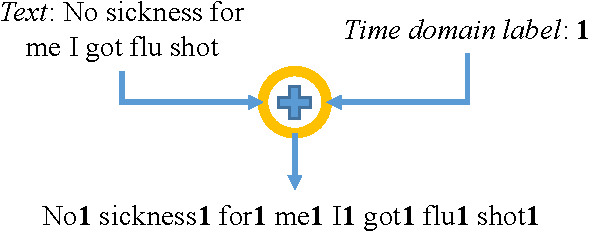
\includegraphics[width=0.75\textwidth]{images/chapter3/domain_doc.pdf}
\caption{The illustration of building domain corpora. We append the document domain label as a suffix to each word in the document.}
\label{chap3:fig:domain}
\end{figure}

FastText learns word embeddings from character n-grams, intended to capture morphological information. As an example, the word ``where1'' from time-domain 1 using character 3-grams would be encoded in fastText as the following seven parts:
\begin{center}
    $<wh, whe, her, ere, re1, e1>, <where1>$
\end{center}

In this way, words with time-domain labels can incorporate temporal identities, while the same words with different domain labels will still share close representations because of similar morphological forms. In this way, we encode temporal identity into word representations while still maintaining the connections of the same words across different time domains. 

In contrast to prior approaches on diachronic embeddings, this concatenative sub-word approach does not explicitly model the ordering of time information, and it cannot encode, for example, that domains that are close in time should have more similarities than domains that are farther away in time.
Despite this limitation, we find experimentally that this approach works competitively while being simpler to implement and faster to train.

\subsection{DWE Evaluation}
\label{chap3:subsec:dweEval}

In this section, we evaluate the effectiveness of our proposed diachronic word embedding.
The goal is to examine if our proposed DWE model can capture the changing sense of words over time.
In all cases, we keep the dimension of word representations as 200.

\subsubsection{Evaluation Data}
We retrieved a newspaper dataset of the New York Times~\cite{yao2018dynamic}.
The dataset contains $99,872$ newspaper articles in 27 years ranging from 1990 to 2016.
We used \textit{RegexpTokenizer} from NLTK~\cite{bird2004nltk} to tokenize the documents that only contain alphabets and numbers.
We then dropped any paragraphs that were less than 5 tokens and filtered out any word was smaller than 5 in the general domain.
With the time information, we grouped documents in every three years: 1990-1992 (90-92); 1993-1995 (93-95); 1996-1998 (96-98); 1999-2001 (99-01); 2002-2004 (02-04); 2005-2007 (05-07); 2008-2010 (08-10); 2011-2013 (11-13); 2014-16 (14-16). 
We show details of preprocessed evaluation data in Table~\ref{chap3:tab:dweEvalData}.
We observe that the frequency of unique words numbers varies across time domains. 
Such variations can impact the vocabulary size and contexts of words, which are important to train word embeddings.

\begin{table}[htp]
\centering
\resizebox{\textwidth}{!}{
    \begin{tabular}{c||cccccccccc}
        \begin{tabular}[c]{@{}c@{}}time\\ interval\end{tabular} & 90-92 & 93-95 & 96-98 & 99-01 & 02-04 & 05-07 & 08-10 & 11-13 & 14-16 & ALL \\\hline\hline
        \#doc & 9770 & 9741 & 9975 & 12209 & 12241 & 11360 & 12240 & 12376 & 9938 & 99850 \\
        \#uw & 41688 & 42213 & 43017 & 48011 & 52016 & 51000 & 50522 & 53368 & 50229 & 128333 \\
        \#awpd & 590 & 600 & 600 & 615 & 710 & 692 & 712 & 781 & 849 & 686 \\
    \end{tabular}
}
\caption{Data stats across each temporal and the general domain, where $\#doc$ is the number of documents, $\#uw$ refers to the unique numbers of words in the domain and $\#awpd$ means the average number of words per document.}
\label{chap3:tab:dweEvalData}
\end{table}


\subsubsection{Baselines}
\label{chap3:subsec:dweBaselines}

% discuss the methods
% how we implement the method, what are their features

\paragraph{Static.} 
We train the word2vec model~\cite{mikolov2013distributed} on the entire corpus without considering time information.
The training parameters keep their default values in Gensim~\cite{rehurek2010software}.

\paragraph{Linear.} 
Kulkarni et al.~\cite{kulkarni2015statistically} proposed a linear alignment method. The approach first extracts k nearest neighbors of words in both source and target domains and then uses a linear regression projection to minimize the distance between those word representations. We use the \textit{NearestNeighbors} from scikit-learn~\cite{pedregosa2011scikit} and \textit{WLS} function from StatsModels to implement the baseline.

\paragraph{Procrustes.} 
Hamilton et al.~\cite{hamilton2016diachronic} used orthogonal Procrustes to align yearly embedding models. We implement the model via \textit{procurstes} function in SciPy~\cite{scipy_2001}. We align embedding models of other temporal intervals towards the embedding model in the latest time interval.

\paragraph{Hierarchy.} 
Zhang et al.~\cite{zhang2017temporal} developed a weighted linear transformation method weighted by hierarchical clusters of words. To build transformation matrices, the method first chooses the top 5\% frequent terms in the intersections of vocabularies among the corpora across temporal domains. Then it calculates the weights by the hop distance in the clusters. Finally, the method can learn weighted transformation matrices to align temporal domains together. To implement the model, we used \textit{Ridge} and \textit{linkage} functions from scikit-learn~\cite{pedregosa2011scikit} and SciPy~\cite{scipy_2001} respectively. We set the k as 0, the weight of l2-norm as 0.05 and leave the rest parameters as default.

\paragraph{DW2V.} 
Yao et al.~\cite{yao2018dynamic} designed a joint optimization problem that minimizes distances between the embeddings and positive point-wise mutual information (PPMI) and distances between every pair of temporal domain's static embeddings. We follow the same parameter settings in their source codes.\footnote{\url{https://github.com/yifan0sun/DynamicWord2Vec}}

\subsubsection{Empirical Results}

We present the evaluation method, metrics and results in this section.
The evaluation set is from the \textit{DW2V}~\cite{yao2018dynamic}, which measures if the embedding models can categorize words their correct meanings across yearly domains. 
The test set contains $1,888$ entries with three different columns: word, section label and year.
The section label has 11 different categories and indicates close meanings of words at certain years in the New York Times, for example, ``adobe'' is under the ``Technology'' section label in 2011.
The year is the time information when the word and section label were generated.
We adjust the year label to the time domain schema.
For example, if the year is 2013, we will convert it to 2011-13.

$$F_\beta = \frac{(\beta^2 + 1) * Precision * Recall}{\beta^2*Precision + Recall}$$

We use the F$_\beta$ to measure the effectiveness of the embedding models on the test set.
Following~\cite{yao2018dynamic}, we set $\beta$ as 1.
By using \textit{SpectralClustering} in scikit-learn~\cite{pedregosa2011scikit}, we first apply the clustering algorithm to group the test words with three different cluster sizes, 10, 15 and 20. 
We set the affinity as cosine and leave other parameters as defaults.
To measure the cluster quality, we then select every two words from the test sets without repetition.
We count the pair as a correct option if the two words share the same section label and from the same cluster or if two words are not the same section label and from the different clusters.
Otherwise, we will count the selection as the wrong option.
Finally, we can apply the F$_\beta$ to measure the quality of clusters and compare the embedding models in Table~\ref{chap3:tab:dweEval}.

\begin{table}[htp]
\centering
\begin{tabular}{c||ccc}
Method & 10 Clusters & 15 Clusters & 20 Clusters \\\hline\hline
Static & .657 & .668 & .655 \\
Linear & .702 & .719 & .765 \\
Procrustes & .628 & .681 & .668 \\
Hierarchy & .636 & .809 & .878 \\
DW2V & .809 & .843 & .854 \\
Ours & \textbf{.810} & \textbf{.916} & \textbf{.905}
\end{tabular}
\caption{Performance evaluation using $F_\beta$.}
\label{chap3:tab:dweEval}
\end{table}

% a brief discussion of the evaluation and the promising results we get so far.
Our method consistently outperforms the other methods and gain about 3.37 absolute percentage improvements. We can also find that a larger cluster generally has better results than a smaller cluster number.


\subsection{Analysis 5: Semantic Distribution Shift using DWE}

\begin{figure}[tb!]
\centering
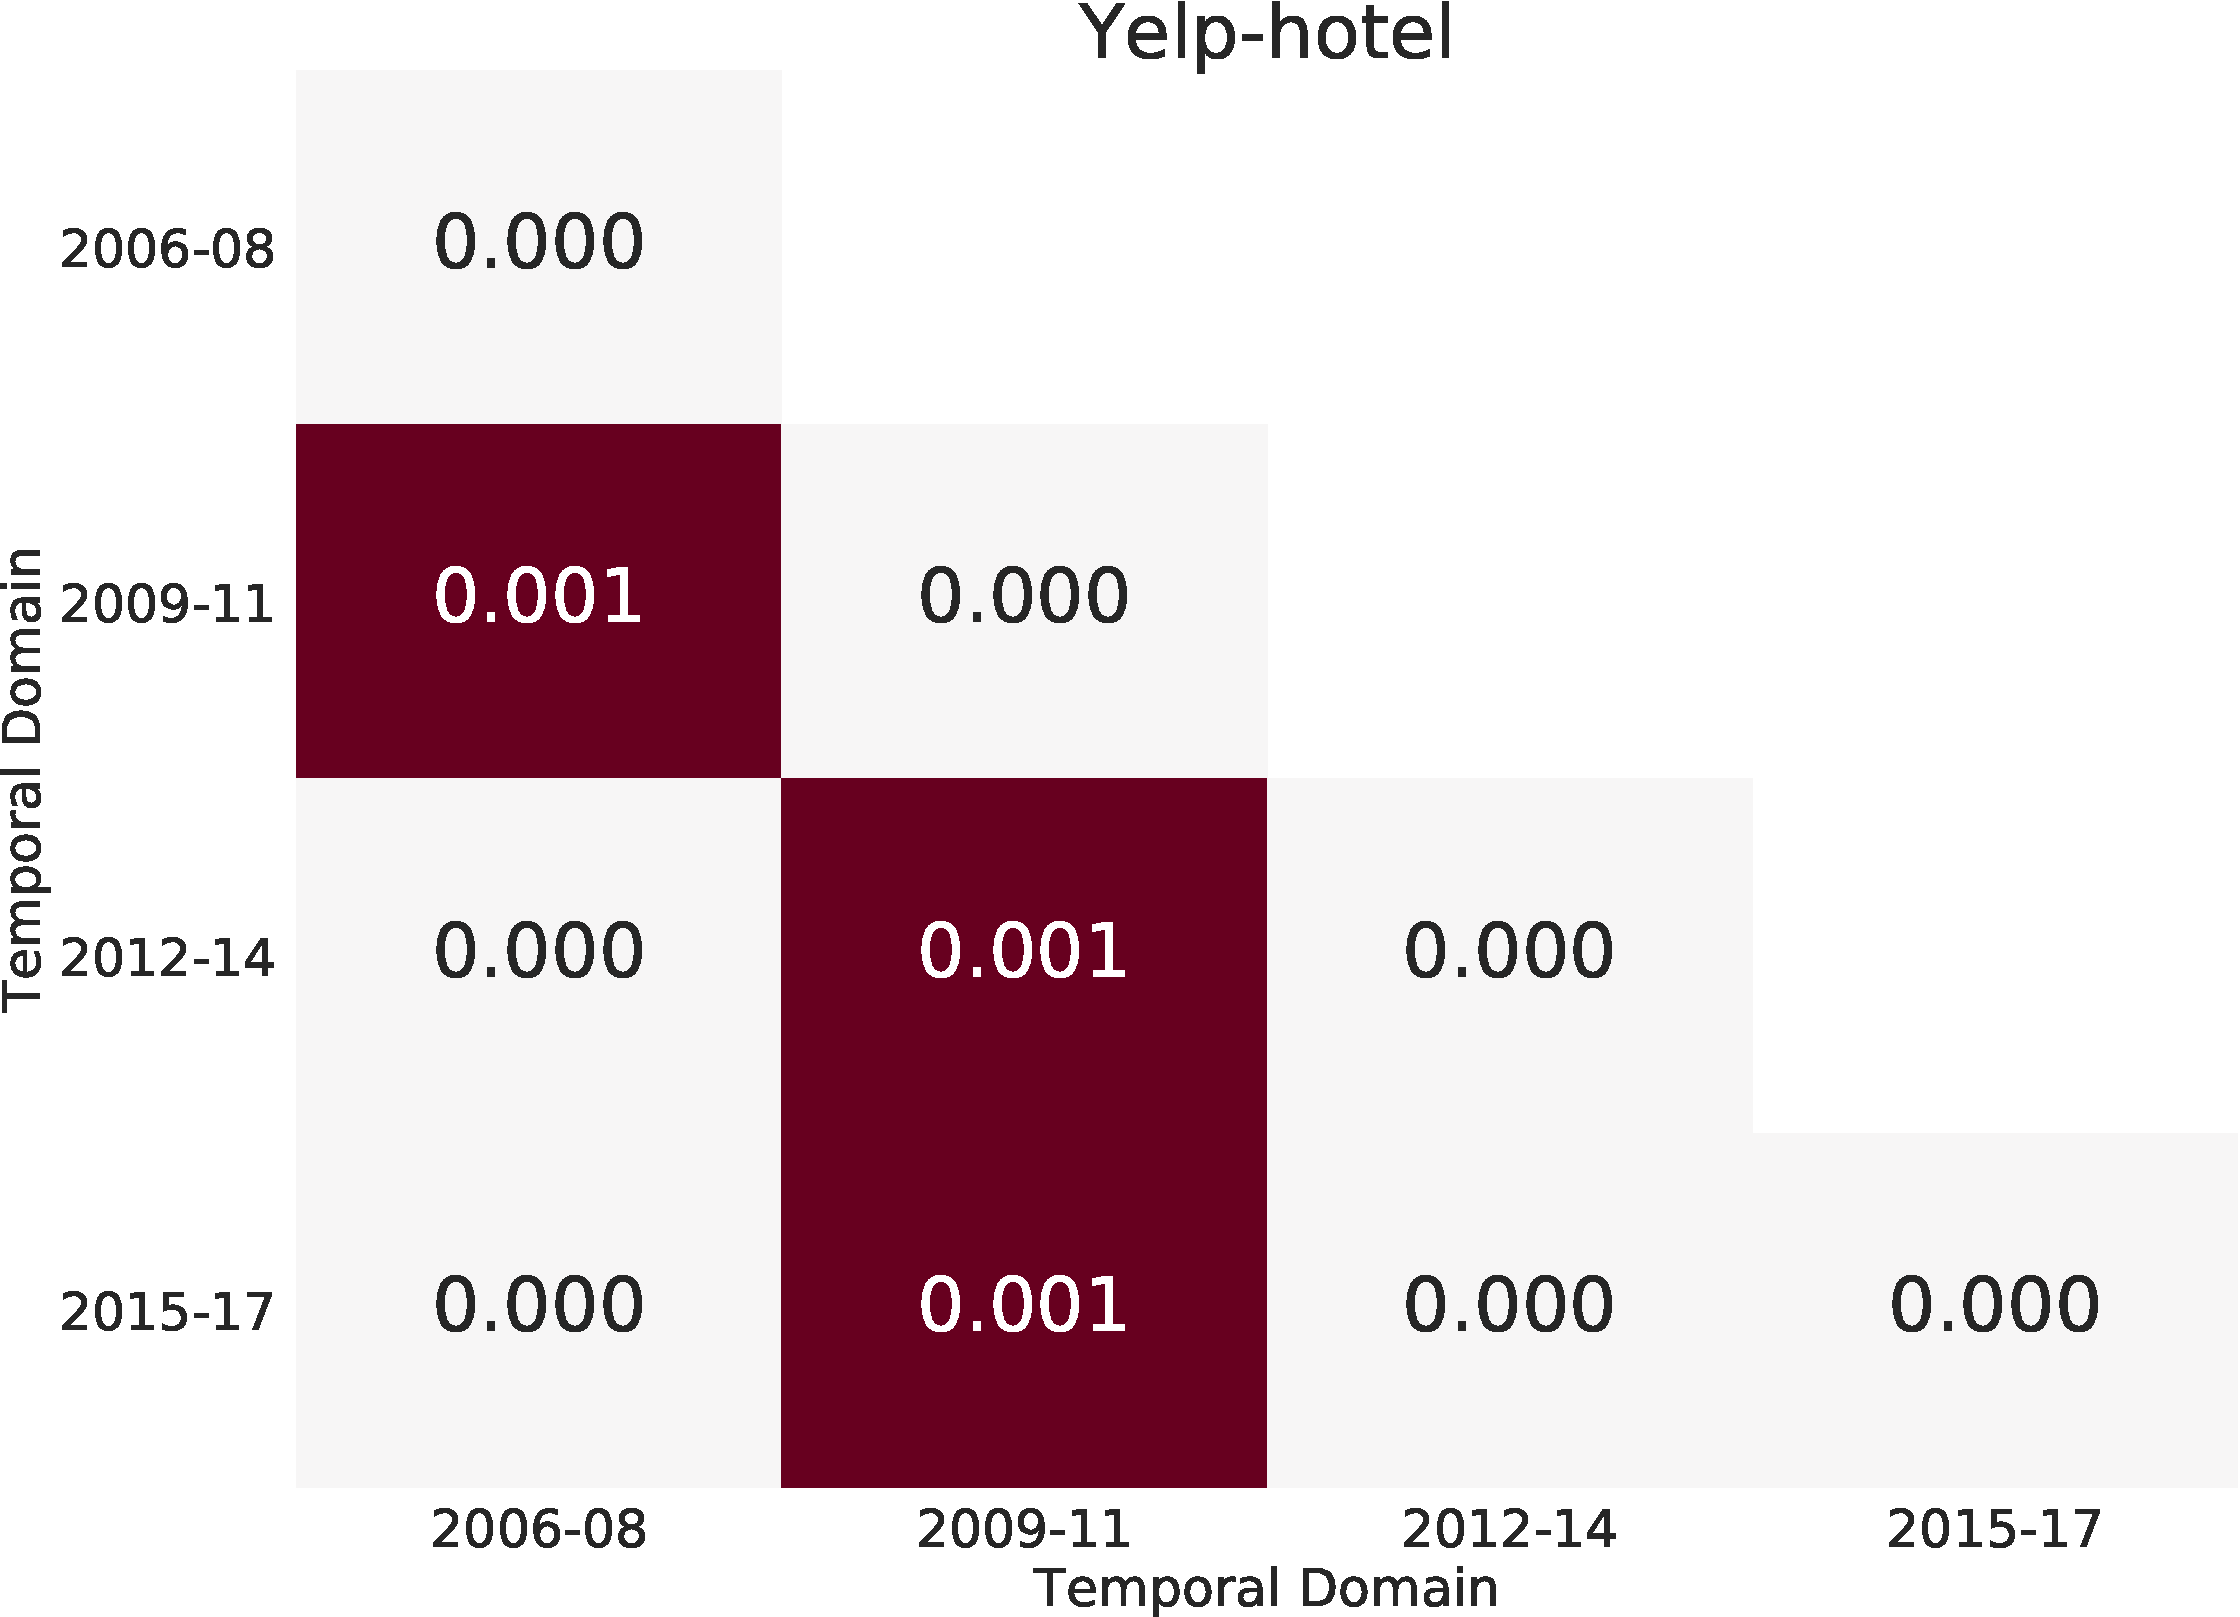
\includegraphics[width=0.48\textwidth]{images/chapter3/sm_shift/yelp_hotel_year_freq.pdf}
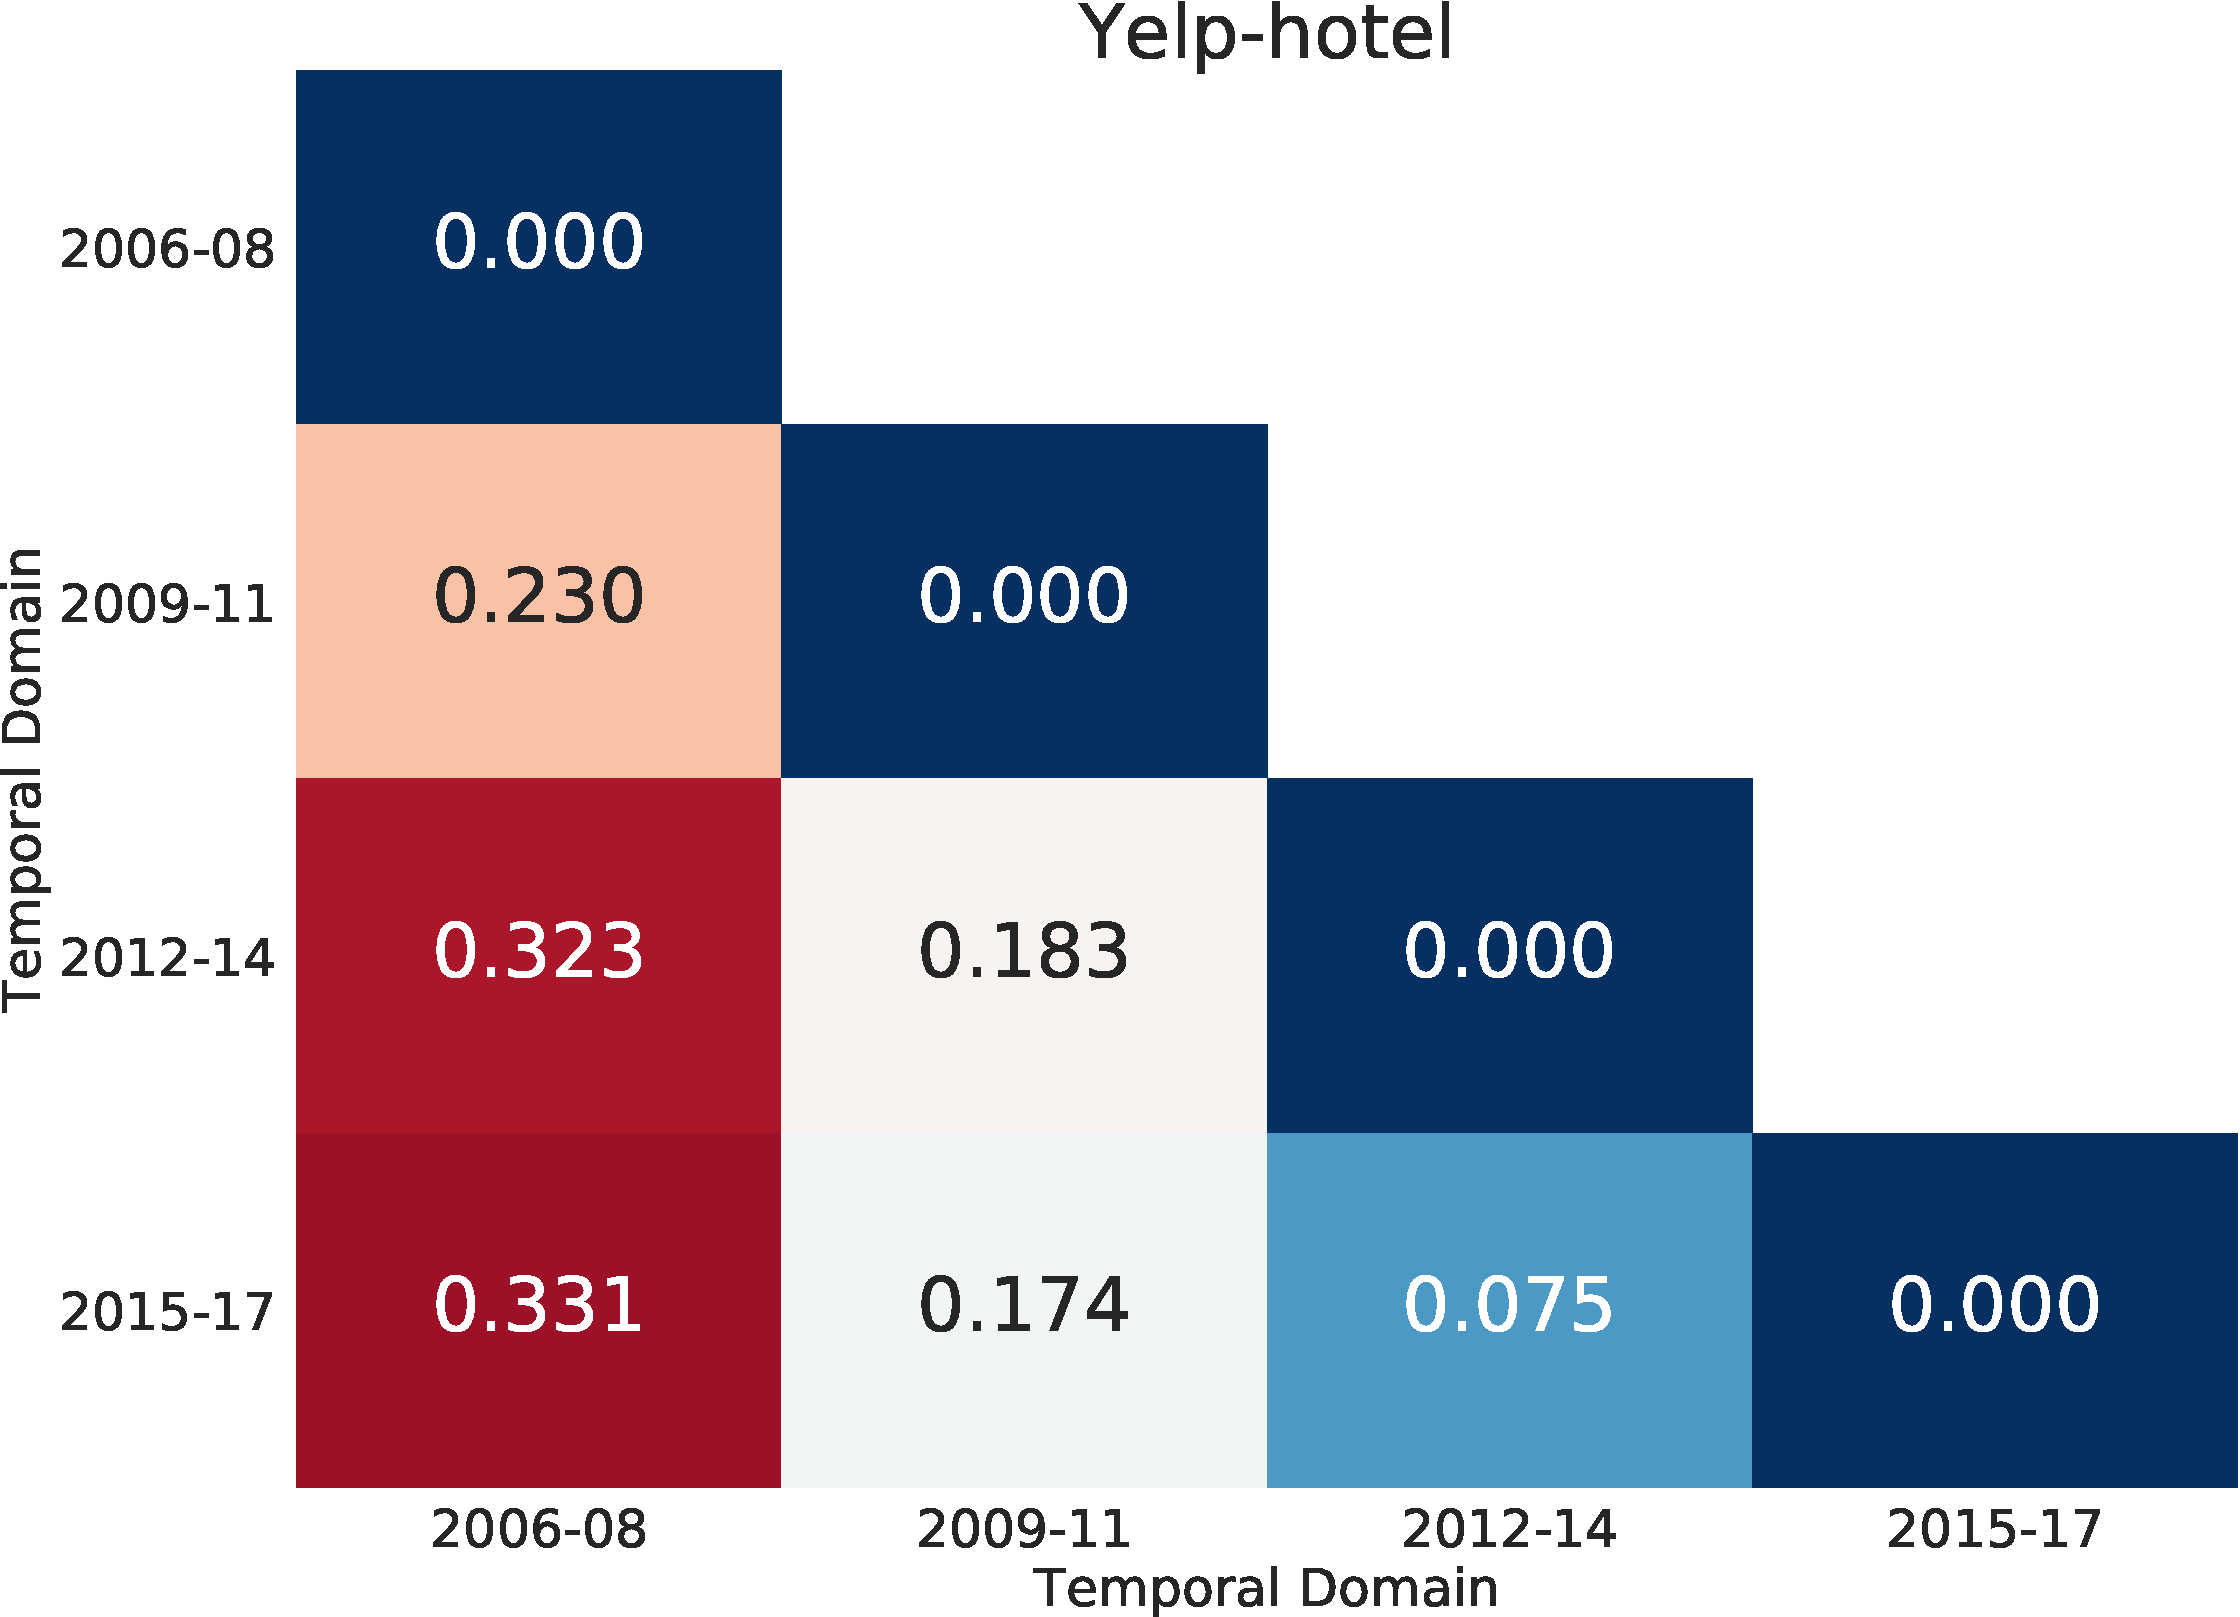
\includegraphics[width=0.48\textwidth]{images/chapter3/sm_shift/yelp_hotel_year_mi.pdf}
\caption{Semantic distribution shifts comparison between the top and most frequent words via Wasserstein distance. We present Yelp-hotel data for the illustration purposes and omit the other data due to space limits. The left is the semantic distribution shift for frequent words, the right is for top words ranked by mutual information. The higher score indicates higher shift.}
\label{chap3:fig:sm_shift}
\end{figure}

Using our proposed approach to constructing diachronic word embeddings,
we now consider how these embeddings can be used to further analyze language shift.

The Law of Conformity states a negative correlation between word frequency and meaning change~\cite{hamilton2016diachronic}; however, \cite{dubossarsky2017outta} shows that word frequency does play an important role in the semantic change, even though a small one. 
Diachronic embeddings have been used to measure the semantic shift using linear interpolation (regression)~\cite{hamilton2016diachronic}. 
Here, we re-examine this issue from another view, the distance of semantic distributions, which views the word embeddings as semantic distributions and measures how the word embeddings vary across time.

As in Section~\ref{chap3:subsec:ctt_shift},
we choose the top 1,000 important words ranked by mutual information, as well as a control group of the 1,000 most frequent words in each corpus.  We find that overlap between the 1,000 most important and most frequent words are 0\% across every dataset. This suggests that the most frequent words are not predictive for classification. 
We use our proposed method to train 200-dimensional diachronic word embeddings and extract diachronic word representations for both important and most frequent words and leave 0s to the words that do not appear within a temporal interval. 
Finally, we use the Wasserstein distance~\cite{vallender1974calculation} to measure the differences across temporal domains.
Wasserstein distance or Earth Mover's distance~\cite{vallender1974calculation} measures the distribution differences between source and target domains,
and thus here it measures semantic distribution shifts across time. 

We show temporal distribution shifts in Figure~\ref{chap3:fig:sm_shift}, 
and we observe two interesting findings. 
First, closer time intervals show less semantic distribution shift, which aligns with our analysis in Sections~\ref{chap3:subsec:wusage} and~\ref{chap3:subsec:ctt_shift}. Second, we observe that the frequent words have much smaller semantic distribution shifts than the top features selected by mutual information. 

To verify this second observation statistically, we conduct a two-tailed t-test on the Yelp-hotel case to test our null hypothesis that the semantic distribution change is not significant. We separately compare the distribution distances of both frequent and top feature words with 0, which indicates no shift. Finally, the test results show p-value=0.076 for the frequent words and p-value=0.0038 for top feature words. Therefore, we reject the null hypothesis of top feature words at a 95\% confidence level while we cannot reject the null hypothesis of frequent words.


\subsubsection{Comparing Different Ways to Measure Temporal Shifts}

\begin{table*}[ht]
\centering
\begin{tabular}{c||cccccc}
Correlation & Amazon  & Dianping & Economy & Twitter & Yelp-hotel & Yelp-rest \\\hline\hline
Usage-DD    & -.901* & .160    & -.106  & .028   & -.943*    & -.923*   \\
Context-DD  & -.989* & -.987*   & -.108  & .023   & -.949*    & -.960*  \\
Usage-Context  & .926* & -.009   & .600*  & .979*   & .950*    & .955*  
\end{tabular}
\caption{The correlations between word usages overlaps (Usage) and distribution distance (DD) as well as context overlaps (Context) and distribution distance (DD). The star sign (*) indicates p-value is less than .05.}
\label{chap3:tab:corr}
\end{table*}

We have presented language shifts across time domains based on word usage overlap (Section~\ref{chap3:subsec:wusage}), context overlap (Section~\ref{chap3:subsec:ctt_shift}), topic change (Section~\ref{chap3:subsec:topic}) and distribution distance (this section). However, it is not clear if these different metrics are measuring the same information. To understand this further, we calculate the Pearson correlation coefficient to measure the relationships between each pair of metrics. 
We show correlations in Table~\ref{chap3:tab:corr}. We observe negative correlations between the two overlap measures (higher means more shift) and distribution distance (lower means less shift),
and a positive correlation between word usage and context overlaps.
These results show that the three metrics are related, though there are some datasets where the correlations are low.


\subsection{Model for Temporality Adaptation}
\label{chap3:sec:model}

\begin{figure*}[tb!]
\centering
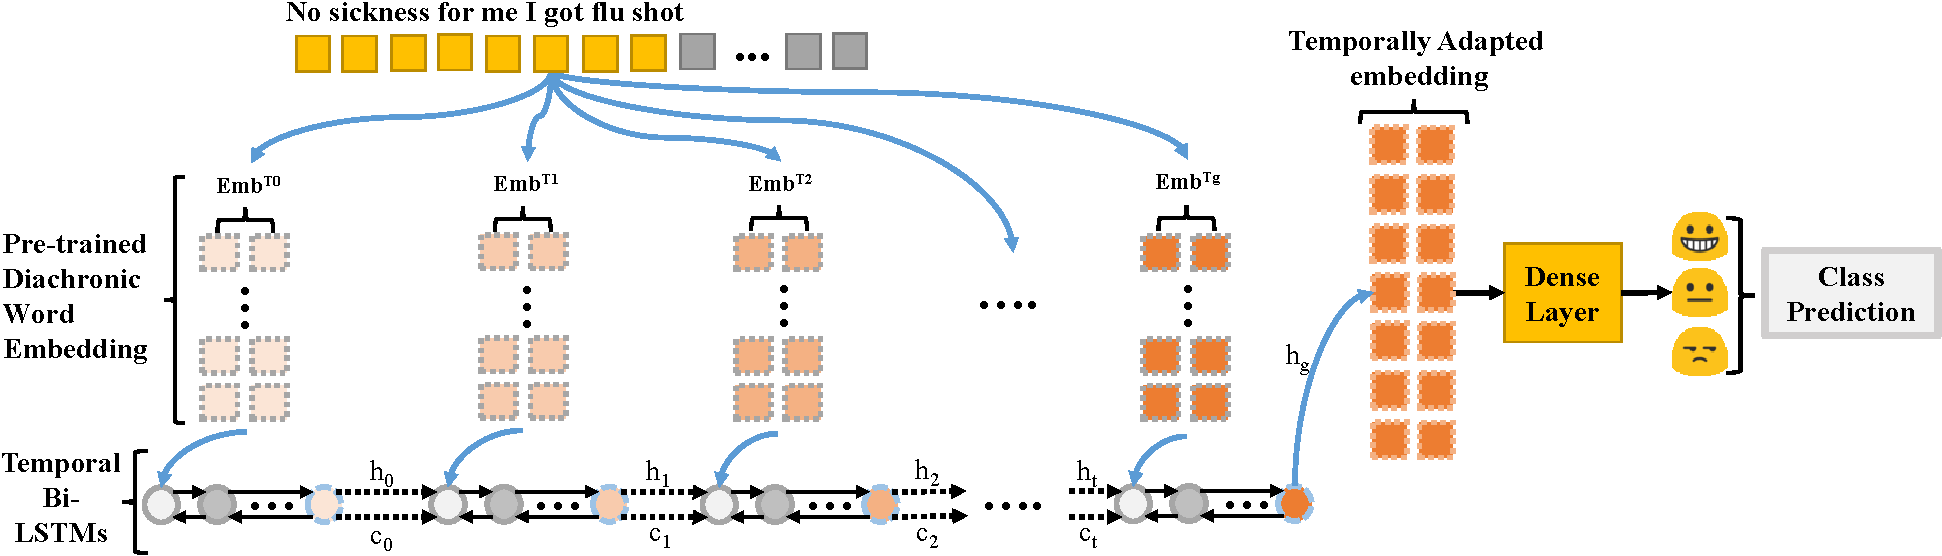
\includegraphics[scale=0.47]{./images/chapter3/model.pdf}
\caption{Architecture of the Neural Temporality Adaptation Model (NTAM). 
NTAM is initialized with $T$ diachronic word embeddings ($Emb^{Tt}, t\in T$) plus one general word embedding ($Emb^{Tg}$). The hidden state ($h_t, t\in T$) and memory cell ($c_t$) will excite and initialize the following Bi-LSTM. We feed the final hidden state ($h_g$, $g$ refers to general domain) to the following learning phase.}
\label{chap3:fig:model}
\end{figure*}

We construct a document classification model that assumes the language used to describe document categories will evolve; for example newer documents may use emoji to express opinions, while older documents would not contain these features.
Our goal is to build document classifiers with time-invariant features and are thus robust to language shift. 

Our previous work~\cite{huang2018examining} on temporality adaptation for $n$-gram classifiers used a domain adaptation approach~\cite{daume2007frustratingly} where 
each time interval is treated as a domain.
This approach created $T+1$ versions of the feature set, one for each of the $T$ time domains, and one domain-independent feature set.
This allows the model to learn which features are associated with specific domains, while the domain-independent parameters can be used for future data.
We analogously apply this idea to the neural setting, where we construct $T+1$ different representations, at both the word level (using diachronic word embeddings) and the document level.
Moreover, we use a time-driven learning process that models
the shift of word representations as a gradual process of adapting representations to new data while starting with old information.

We thus present the {\bf Neural Temporality Adaptation Model (NTAM)} (Figure~\ref{chap3:fig:model}) based on three strategies: diachronic word embeddings (Section~\ref{chap3:sec:dwe}), $T+1$ views of inputs and a time-driven learning process.
This model can learn language shifts and time-invariant representations of documents for classification.

\paragraph{T+1 views of inputs.}
Analogous to the approach of \cite{daume2007frustratingly} for non-neural classifiers, 
we create $T+1$ word representations, where $T$ refers to the number of diachronic domain embeddings and 1 refers to a general embedding, which trains word embeddings on the whole corpus without time labels. Our intuition is to use time-specific embeddings to provide documents from different time intervals with different views of semantic meaning. 
We train diachronic word embeddings using our proposed method via fastText, though we also experiment with other approaches. 
We initialize the model with the domain-specific embeddings and the general word embedding. The model will encode input documents into $T+1$ views of word representations. 
The $T+1$ embeddings provide diverse views of input words, which are fed to the rest of the neural architecture, leaving the model to optimize representations automatically.

\paragraph{Time-driven learning process.}
To learn temporal variations for document representations, we propose a series of $T+1$ continuously temporal Bidirectional Long Short Term Memory (Bi-LSTM) models~\cite{hochreiter1997long}. The first $T$ Bi-LSTMs correspond to the $T$ time domains and the last Bi-LSTM corresponds to the general view of input documents and outputs final document representations. Similar to how the diachronic word embeddings encode input words into multiple views of time domains, we use $T+1$ Bi-LSTMs to learn diachronic views of document representations. 

To capture the semantic shifts across time domains, our intuition is to model the dynamic process. The memory mechanism of LSTM fits our needs, which optimizes the balance across different time patterns via non-linear computations. While each Bi-LSTM reads through tokens in its input document, we feed the previous Bi-LSTM's hidden state and memory cell to excite the learning process of the subsequent Bi-LSTM. The final Bi-LSTM learns jointly the previous shift patterns of document representations with the general embedding view of documents and outputs its final document representation $h_g$. 

The final document representation is fed into a dense layer with a non-linear activation function. We use outputs of the dense layer for document class prediction,
where we use one-hot encoding to represent document labels and use the softmax function for class predictions. Finally, we use categorical cross-entropy as the loss function.



\subsection{Experiments}
\label{chap3:sec:dweExp}

We conduct experiments on the task of document classification.
We split the data chronologically to simulate the realistic scenario where a classifier is trained on older data and tested on newer data. 
Thus, the first $T-1$ time domains are used for training;
the last time domain is split into two equal-sized sets for development and testing.
The final data details are described in Table~\ref{chap3:table:statics}.

\begin{table}[ht]
 \centering
 %\resizebox{\columnwidth}{!}{
    \begin{tabular}{c|ccc}
    \hline\hline
    Datasets & Train & Dev. & Test\\
    \hline
    Amazon & 59,399 & 11,880 & 11,880 \\
    Dianping & 503,330 & 83,889 & 83,889 \\
    Economy & 4,774 & 596 & 596\\
    Twitter & 1,632 & 272 & 272\\
    Yelp-hotel & 20,975 & 6,993 & 6,993 \\
    Yelp-rest & 106,943 & 35,648 & 35,648 \\
    \hline
    \end{tabular}
    %}
    \caption{Data statistics of the six corpora. We show the number of documents in each split.}
    \label{chap3:table:statics}
\end{table}


\subsubsection{Implementation and Training}
We implement classification models using Keras~\cite{chollet2015keras} and scikit-learn~\cite{pedregosa2011scikit}. We select the top 15K words by frequency and set the other words as ``unk''. The models are trained for 15 epochs with a batch size of 64. Each document is padded to 60 tokens. We set the Bi-LSTM output to 200 dimensions. We choose ReLU~\cite{hahnloser2000digital} as the activation function of the dense layer and 0.2 as our default dropout rate~\cite{srivastava2014dropout}. The dense layer outputs 200 dimensions for final document class prediction. We select cross-entropy as our default loss function, and we optimize model parameters via RMSprop~\cite{tieleman2012lecture} with the learning rate as 0.0001. Unless otherwise stated, we leave the other parameters as defaults.

\subsubsection{No Adaptation Baselines}
To ensure fair comparisons, we use the same settings across all models. We compare our proposed model to seven baselines, where three standard classifiers do not perform temporality adaptation.

\paragraph{LR.} 
We extract 1- and 2-gram features on the corpora with the most frequent 15K features. We then build a logistic regression classifier using \texttt{LogisticRegression} from scikit-learn~\cite{pedregosa2011scikit} with default parameters.

\paragraph{CNN.} 
We implement the Convolutional Neural Network (CNN) classifier described in~\cite{kim2014convolutional}. To stay consistent, we initialize the model with pre-trained word embeddings~\cite{bojanowski2017enriching} that were trained on the same datasets as diachronic embeddings. We only keep the 15K most frequent words and replace the rest with an ``unk'' token. 
We set the model optimizer as Adam~\cite{kingma2014adam}. 

\paragraph{Bi-LSTM.} 
We build a bi-directional Long Short Term Memory (bi-LSTM)~\cite{hochreiter1997long} classifier to examine the effectiveness of the temporal learning process in our proposed model. The classifier is initialized with the pre-trained word embeddings.

\subsubsection{Domain Adaptation Baselines}

\paragraph{FEDA.} 
We adapt for time domains using the ``frustratingly easy'' domain adaptation (FEDA) method~\cite{daume2007frustratingly}. 
This method is the same as our proposed method in Section~\ref{chap3:sec:fa}.
The feature set is augmented such that each feature has a domain-specific version of the feature for each time domain, as well as a general domain-independent version of the feature.
The values of features are set to the original feature value for the domain-independent feature and the domain-specific features that apply to the document, while domain-specific features for documents that do not belong to that domain are set to $0$.
At test time, we only use the general, domain-independent features. 
We use the same feature extraction procedures and the same logistic regression classifier as the \textit{LR} baseline.

\paragraph{DANN.} 
We consider the domain adversarial training network~\cite{ganin2016domain} (DANN) on the time adaptation task. We re-implement the same network and set domain prediction as predicting the time domain label while keeping the document label prediction to the default. We use the model from the epoch when the model achieves the best result on the development set for the final model.

\paragraph{RCNN \& HAN.} 
He et al.~\cite{he2018time} propose an evolving framework to train document classifiers. We re-implement two classifiers, RCNN and HAN with a diachronic propagation learning strategy, which achieved the best performances in their paper. The RCNN~\cite{lai2015recurrent} classifier integrates both LSTM and CNN, and the HAN~\cite{yang2016hierarchical} classifiers use hierarchical attention neural architectures. We keep the two models with the same parameters as their open-sourced code and initialize the two models with pre-trained 200-dimensional word embeddings~\cite{bojanowski2017enriching}. We apply Adam and RMsprop for RCNN and HAN respectively, because the two optimizers perform much better on validation sets than the stochastic gradient descent optimizer used in the original paper. The work is close to our work but there are three major differences:
\begin{itemize}
    \item Time invariance. We train one unified model with diachronic adaptation by using a time-independent representation (the 1 of the $T+1$ representations) to learn a time-invariant classifier that can be used for future data. In contrast, these baselines learn $T-1$ models, where they train one model for each time domain.
    \item Diachronic word embeddings. Our method uses diachronic word embeddings to encode inputs in $T+1$ different views. The baseline encoding is based on only the current embedding space and therefore might not capture embedding shifts over time.
    \item Learning process. The baseline learns a weighted sum between the intermediate layer's outputs between the previous model and the current model. In contrast, we deploy the $T+1$ Bi-LSTMs to jointly learn time dependencies across all time intervals.
\end{itemize} 


\begin{table*}[t]
\centering
\begin{tabular}{c||ccc||cccc||c}
 & \multicolumn{3}{c||}{Baselines (No adaptation)} & \multicolumn{4}{c||}{Baselines (Adaptation)} & Our Model \\
Data & LR & CNN & Bi-LSTM & FEDA & DANN & HAN & RCNN & NTAM\\\hline\hline
Twitter & .874 & .873 & .879 & .890 & .851 & .847 & .869 & \textbf{.898} \\
Economy & .699 & .707 & .692 & .686 & .687 & .690 & .697 &  \textbf{.711} \\
Yelp-rest & .818 & .756 & .787 & \textbf{.831} & .736 & .794 & .782 & .828 \\
Yelp-hotel & .773 & .753 & .758 & \textbf{.811} & .733 & .740 & .762 & .790 \\
Amazon & .778 & .762 & .771 & .782 & .686 & .748 & .782 & \textbf{.808} \\
Dianping & .710 & .715 & .706 & .687 & .686 & .699 & .692 & \textbf{.738}
\end{tabular}
\caption{Performance of different models evaluated with weighted F1 scores. For each dataset, the best score is bolded. 
LR and FEDA are non-neural $n$-gram models, while the others are neural models.
}
\label{chap3:tab:results}
\end{table*}


\begin{table*}[t]
\centering
\begin{tabular}{c||cccc||cccc}
 & \multicolumn{4}{c||}{RCNN} & \multicolumn{4}{c}{NTAM} \\
Data & Incre & Linear & Procrustes & Subword & Incre & Linear & Procrustes & Subword\\\hline\hline
Twitter & -0.7 & +1.4 & -0.2 & -0.8 & +1.4 & -0.3 & +1.7 & +3.5\\
Economy & +0.5 & 0.0 & -0.7 & +0.4 & -0.3 & -1.0 & -0.5 & +0.3\\
Yelp-rest & +1.4 & +0.1 & -1.9 & +2.3 & +1.9 & +1.6 & +1.4 & +4.3\\
Yelp-hotel & -1.5 & -1.2 & -0.5 & -0.2 & -0.7 & -2.0 & -1.8 & +0.8\\
Amazon & +0.2 & +0.2 & -2.0 & +0.5 & -0.8 & -0.7 & -0.8 & +2.1\\
Dianping & +0.4 & +1.6 & +0.7 & +1.0 & +0.8 & +1.8 & +3.4 & +4.2\\\hline\hline
Average & 0.05 & 0.35 & -0.47 & 0.53 & 0.38 & -0.10 & 0.57 & 2.53\\
Median & 0.30 & 0.15 & -0.60 & 0.45 & 0.25 & -0.50 & 0.45 & 2.80\\
\end{tabular}
\caption{Performance gains of two neural temporality adaptation models when they are initialized by diachronic word embeddings as compared to initialization with standard non-diachronic word embeddings. \textit{Subword} refers to our proposed diachronic word embedding in this chapter (Section~\ref{chap3:sec:dwe}). We report absolute percentage increases in weighted F1 score after applying diachronic word embeddings.}
\label{chap3:tab:dia}
\end{table*}


\subsubsection{Results}
\label{chap3:sec:results}


The results of our experiments are shown in Table~\ref{chap3:tab:results}. 
Our proposed approach leads to performance improvements over the baselines on majority of the datasets.
NTAM has the highest performance on 4 out of 6 datasets, while FEDA has the highest performance on the other 2 (while NTAM is the next best for those 2).


The baselines with domain adaptation generally obtain a small performance boost over the baselines without adaptation on temporality. 
Among the non-neural models, the adaptation baseline FEDA outperforms the non-adaptation baseline LR on 4 out of 6 datasets. 
Among the neural models, the best adaptation baseline outperforms the best non-adaptation baseline on 3 out of 6 datasets,
with the RCNN generally outperforming the other baselines.
%The RCNN generally shows improvements over the other neural non-adaptation models on the Yelp and Amazon datasets. 
This indicates that the temporal factor can potentially improve the performance of document classification, and that domain adaptation is a possible approach to temporality adaptation. 

\paragraph{Significance analysis.} 
To verify the improvements of our proposed method NTAM compared to baselines, we conduct a significance analysis to compare our proposed model with the RCNN, which is the closest model to ours. We follow \cite{berg2012empirical} and bootstrap sample 50 pairs of test datasets with replacement. We keep the same data size as the previous experiments in Table~\ref{chap3:tab:results}. We then use the same previous parameters and re-conduct the classification experiments. We format the experimental results as two lists of scores. We conduct a paired t-test to test a null hypothesis that our proposed model does not differ significantly from the RCNN. The test presents a significant result with t(95) = 3.258 and p-value < 0.005. The result suggests rejecting the null hypothesis at a 95\% confidence level.


\subsection{Effectiveness of Diachronic Embeddings}

Lastly, we investigate how diachronic word embeddings affect classifiers.
While NTAM used diachronic word embeddings and other baselines did not,
we also compare to a version of NTAM initialized with regular word embeddings (to understand whether diachronic embeddings are important to the model's performance),
and we also experiment with combining diachronic embeddings with a baseline model (to understand if diachronic embeddings can be used in other classifiers).


We also compare different methods of constructing diachronic word embeddings. In addition to our proposed method in Section~\ref{chap3:sec:dwe}, which uses subword embeddings via fastText,
we consider three other approaches (Section~\ref{chap3:subsec:dweBaselines}).
We use incremental training~\cite{kim2014temporal} (abbreviated \textit{Incre}, using fastText),
linear regression~\cite{kulkarni2015statistically}, implemented in scikit-learn,
and Procrustes~\cite{hamilton2016diachronic}, implemented in SciPy.
We keep the same fastText parameters as in previous experiments and train a word embedding model separately for each time domain, then align the pre-trained embeddings to get final diachronic word embeddings. 
We then re-run the classification task with the new diachronic word embeddings. 
Implementations of the baselines are the same as Section~\ref{chap3:tab:dweEval}.

Table~\ref{chap3:tab:dia} shows the absolute percentage improvement in classification performance when using each diachronic embedding compared to a classifier without diachronic embeddings.
Overall, diachronic embeddings improve classification models.
The diachronic embedding appears to be particularly important for NTAM, improving performance on all 6 datasets with an average increase in performance up to 2.53 points.
The RCNN also benefits from diachronic embeddings, but to a lesser extent, with an improvement on 4 of the 6 datasets.
Comparing the different methods for constructing diachronic embeddings,
we find that our proposed subword method works the best on average for both classifiers. The incremental training method also provides improved performance for both classifiers, while the linear regression and Procrustes approaches have mixed results.


\section{Conclusion}
\label{chap3:sec:conclusion}

In this chapter, we proposed two temporality adaptation methods to improve the temporal robustness of document classifiers via the feature augmentation and diachronic word embedding.
We explore and examine language temporal shifts on seven bilingual corpora from social media to news articles in Section~\ref{chap3:sec:data}. 
As described in Section~\ref{chap3:sec:fa}, We have shown both qualitatively and quantitatively that our proposed FEDA and diachronic word embedding are capable of discovering language shift patterns and improve model productiveness across both seasonal and non-seasonal periods.
We proposed a new framework to train diachronic word embedding via a subword mechanism in Section~\ref{chap3:sec:dwe}.
Evaluations using a clustering task of word analogy show preeminence of our proposed DWE model.
The Section~\ref{chap3:sec:model} presented a new time-driven classification model that encodes documents through the diachronic word embedding. 
